\chapter{Physics Objects}\label{sec:objects}

\section{Electrons}

\subsection{Electron Reconstruction}
\label{sec:eleReco}


Electron candidates are preselected using loose cuts on track-cluster matching observables, so as to preserve the highest possible efficiency while rejecting part of the QCD background. To be considered for the analysis, electrons are required to have a
transverse momentum $p^e_T >$ 7 GeV, a reconstructed $|\eta^e| <$ 2.5, and to satisfy a loose primary vertex 
constraint defined as $d_{xy} < 0.5$ and $d_z < 1$. 
Such electrons are called {\bf loose electrons}.

The early runs in the 2016 data-taking exhibit an tracking inefficiency originating from a reduced hit reconstruction efficiency in the strip detector (``HIP" effect). 
The resulting data-MC discrepancy is corrected using scale factors as is done for the electron selection with data efficiencies measured using the same tag-and-probe technique outlined later (see Section~\ref{sec:eleEffMeas}). 
These studies are carried out by the EGM POG and the results are summarized here.

The electron reconstruction scale factors are shown Fig.~\ref{fig:ele_rec_scale_factors} as a one-dimensional function of the super cluster $\eta$ only, as it was shown that the $\pt$ dependence of the scale factor is negligible. More details on electron reconstruction can be found in Ref.~\cite{ElectronLegacy}. 

\begin{figure}[!htb]
\vspace*{0.3cm}
\begin{center}
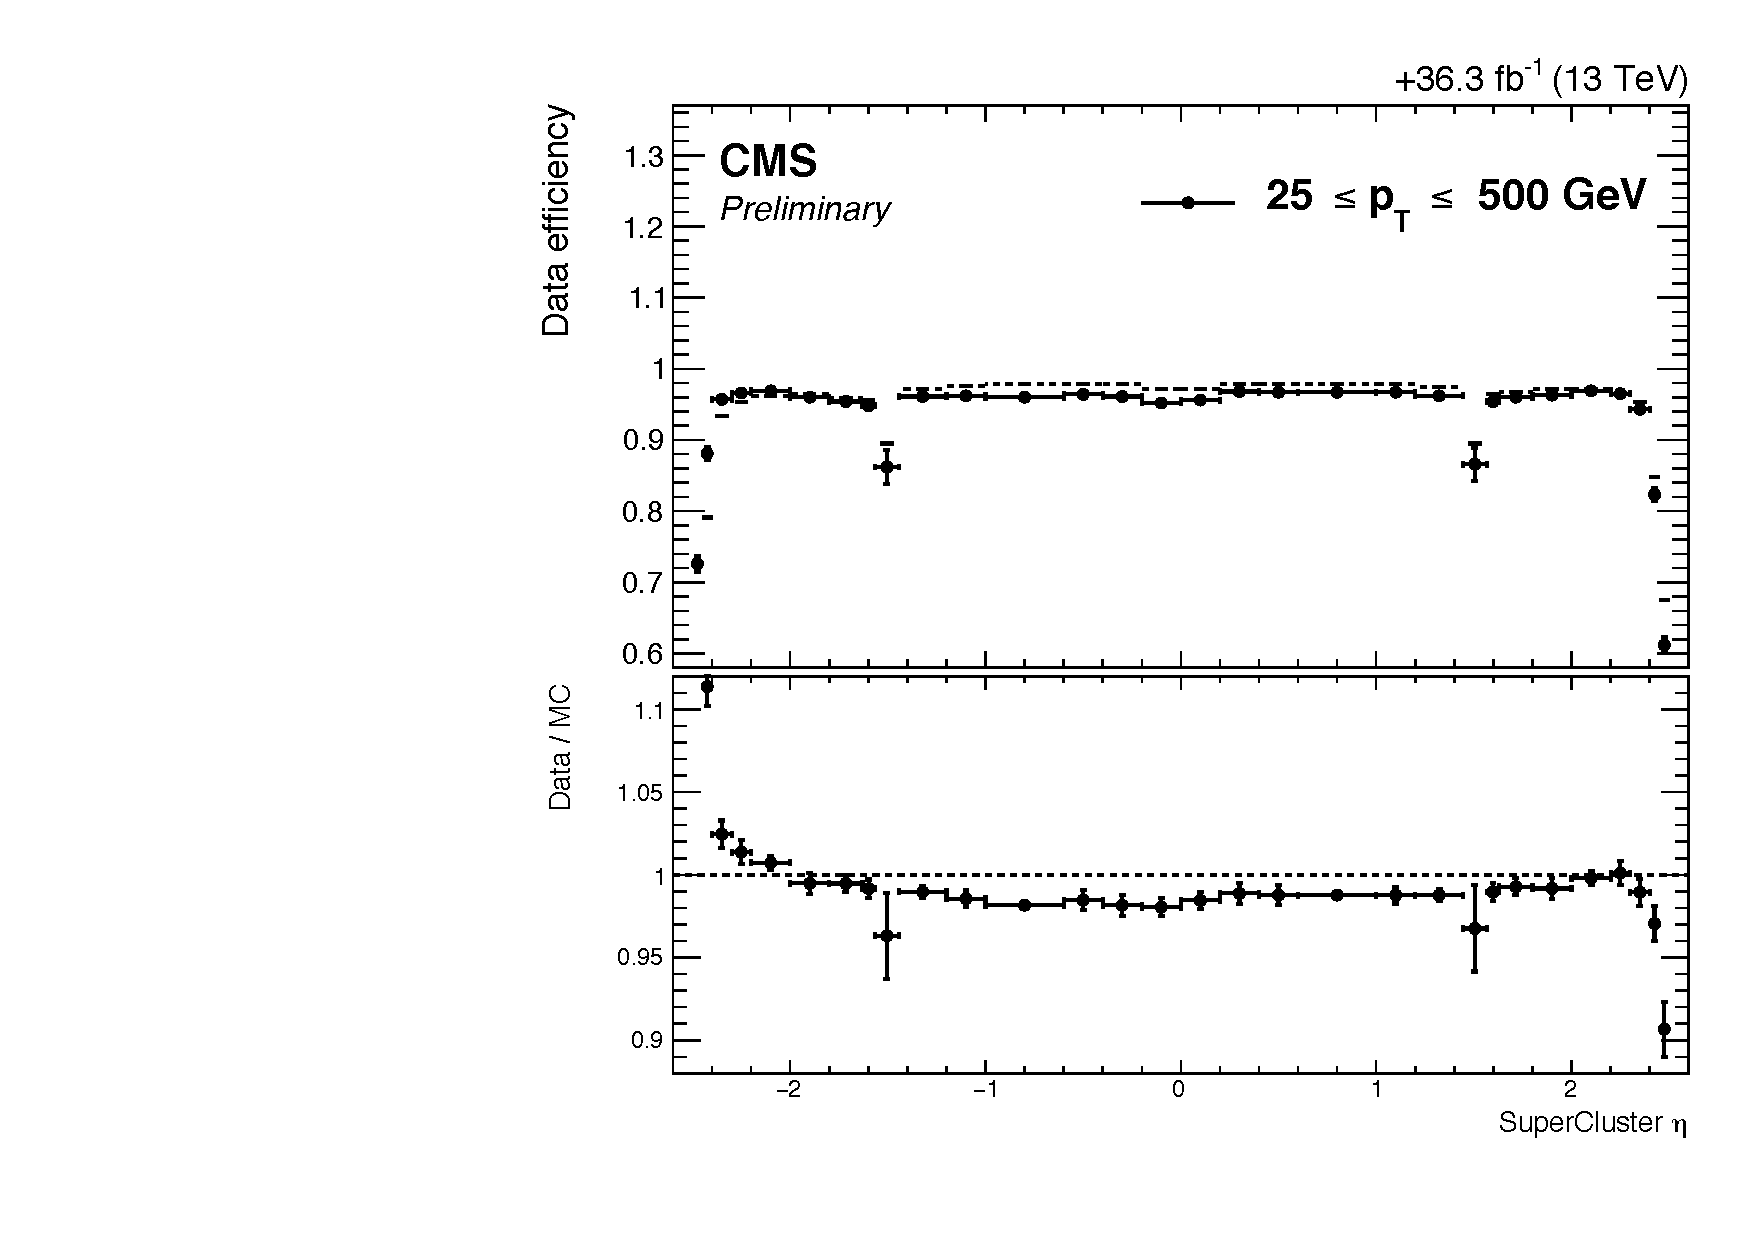
\includegraphics[width=0.6\textwidth]{Figures/Electrons/ele_rec_scale_factors.pdf}
\end{center}
\caption{Electron reconstruction efficiencies efficiency in data versus $\eta$ and data/MC scale factors as provided by the EGM POG.}
\label{fig:ele_rec_scale_factors}
\end{figure}

\subsection{Electron Identification}
\label{sec:eleID}

Reconstructed electrons are identified by means of a Gradient Boosted Decision Tree (GBDT) multivariate classifier algorithm, which exploits observables from the electromagnetic cluster, the matching between the cluster and the electron track as well as observables based exclusively on tracking measurements. 
The BDT has been retrained using CMSSW\_8\_0\_X samples. The classifier is trained on Drell-Yan plus jets MC sample for both signal and background: 

%{
%\resizebox{\textwidth}{!}{%
%\tiny  
%/DYJetsToLL\_M-50\_TuneCUETP8M1\_13TeV-madgraphMLM-pythia8/RunIISpring16DR80-PUSpring16\_80X\_mcRun2\_asymptotic\_2016\_v3\_ext1-v1/
%}}
%{
%\tiny  
%\begin{verbatim}
%/DYJetsToLL_M-50_TuneCUETP8M1_13TeV-madgraphMLM-pythia8/RunIISpring16DR80-PUSpring16_80X_mcRun2_asymptotic_2016_v3_ext1-v1/
%\end{verbatim}
%}

The impact of the retraining of the ID for the 2016 conditions is illustrated in the ROC curves shown in Fig.~\ref{fig:ele_ID_ROC}. Several studies to improve the performance of the MVA for the harsher 2016 running conditions were performed. 
One study considered a new spitting of the BDT training bins, where electrons falling into the gap regions of the ECAL, e.g. the EB-EE transition region, where trained separately from the non-gap electrons. 
No improvement for either population is observed, indicating that the current setup is already able to properly take the significantly differing input distributions in those regions into account. 
Also studied where additional variables including more cluster-shape observables. 
None of these variables helped to improve the performance in the relevant $>95\%$ signal efficiency regime, though up to $20\%$ improved background rejection was seen for $80\%$ working points. 
Finally, the hyper-parameters of the MVA were systematically scanned for their optimal values. The resulting configuration was found to improve the overall performance only marginally by $<10\%$, however, introducing a significant overtraining effect. 
Due to the small gains and large overtraining, it was decided to not modify the hyper-parameters beyond the interface changes coming from changing to the latest 4.2.0 version of the TMVA package.

Figure~\ref{fig:ele_ID_BDT_output} shows the output of the BDT on the training and testing samples for true and fake electrons 
for the high-$p_T$ training bin in the endcap. 
The good agreement between the training and testing distributions is similar across the 6 training bins and indicates that the classifier has not been overtrained.

\begin{figure}[!htb]
\vspace*{0.3cm}
\begin{center}
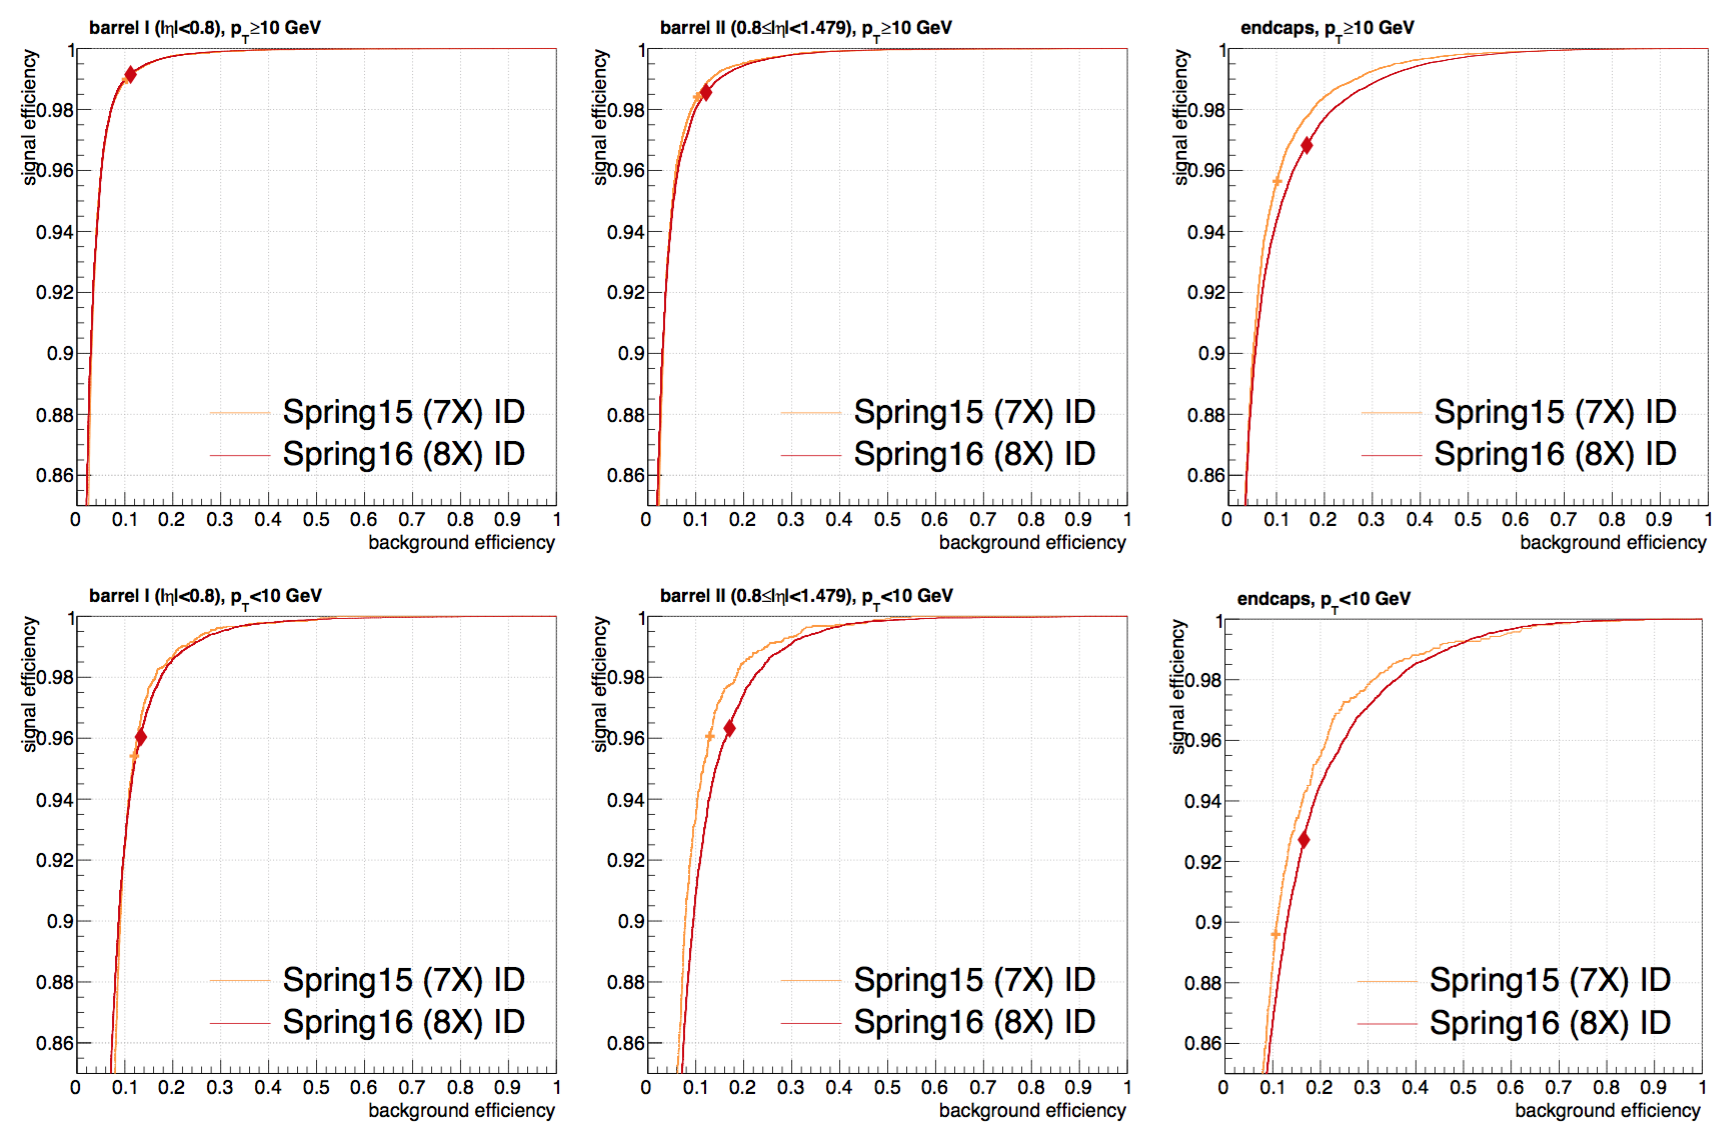
\includegraphics[width=0.80\textwidth]{Figures/Electrons/ele_ROC.png}
\caption{Performance comparison of the MVA trained for the 2015 analysis and the retraining for 2016 conditions. 
The respective working points are indicated by the markers.
\label{fig:ele_ID_ROC}}
\end{center}
\end{figure}

\begin{figure}[!htb]
\vspace*{0.3cm}
\begin{center}
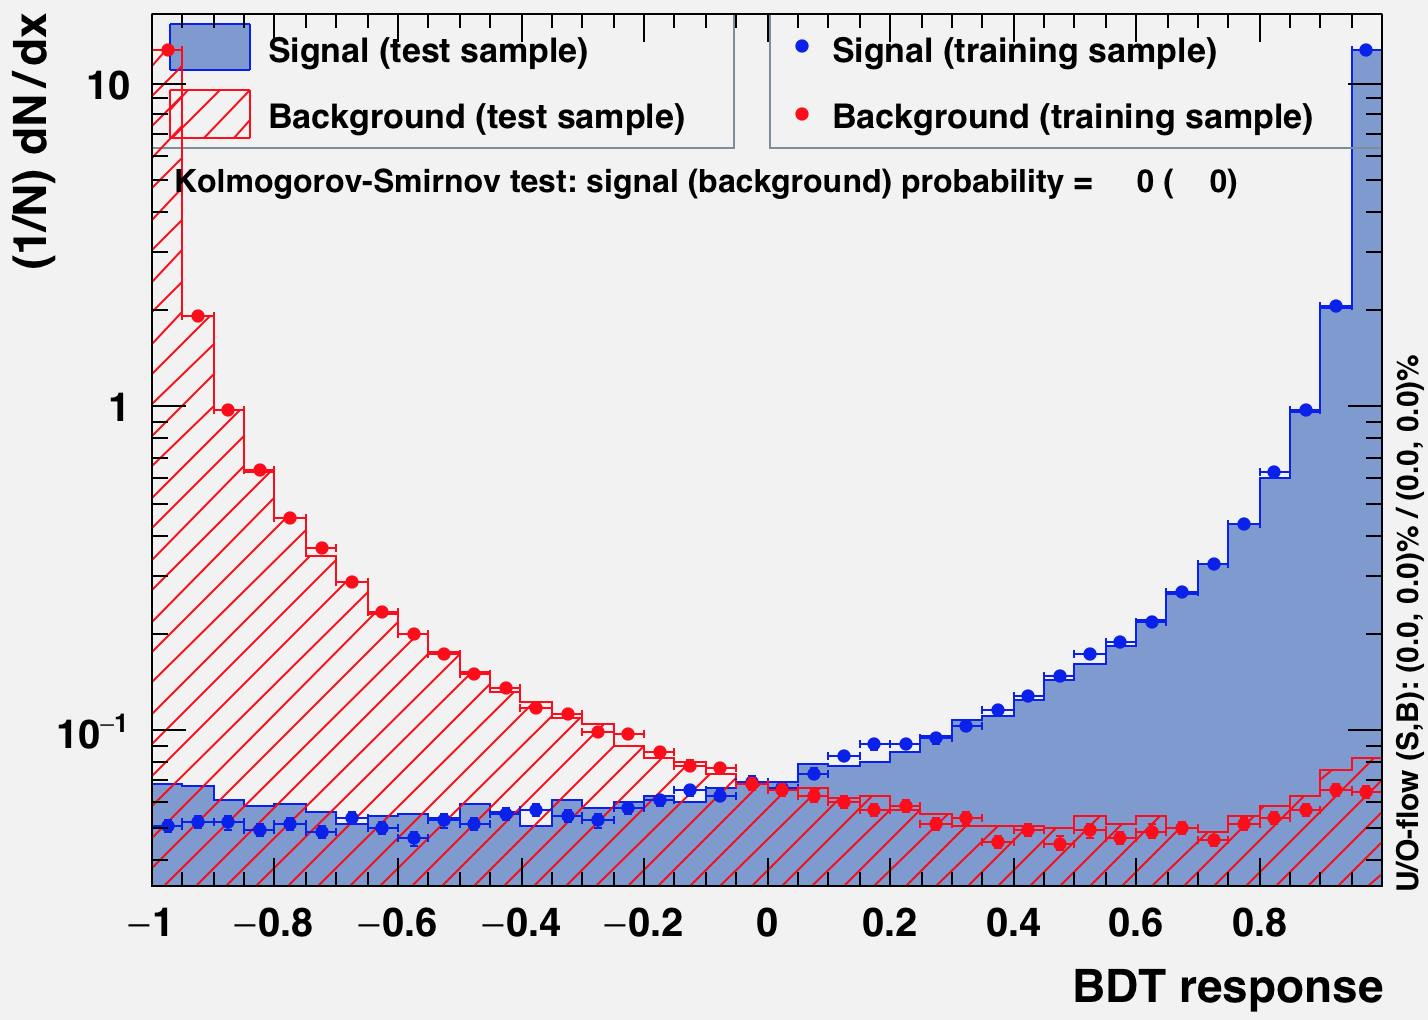
\includegraphics[width=0.5\textwidth]{Figures/Electrons/ele_overtraining.png}
\caption{BDT output for the training and testing sample for true and fake electrons in the high-$p_T$ endcap training bins.
\label{fig:ele_ID_BDT_output}}
\end{center}
\end{figure}

Table~\ref{tab:ele_ID_input_variables} summarizes the full list of observables used as input to the classifier
and table~\ref{tab:ele_ID_WP} lists the cut values applied to the BDT score for the chosen working point. 
For the analysis, we define {\bf tight electrons} as the loose electrons that pass this MVA identification working point. 

 \begin{table}[h!]
\scriptsize
    \centering
\resizebox{\textwidth}{!}{%
    \begin{tabular}{c|l}
\hline %----------------------------------------------------------------------------------------
\hline %----------------------------------------------------------------------------------------
%\multicolumn{4}{|c|}{Datasets}                                                                \\
observable type    &  observable name      	\\
\hline %----------------------------------------------------------------------------------------

\multirow{6}{*}{cluster shape}
	&  RMS of the energy-crystal number spectrum along $\eta$ and $\varphi$; $\sigma_{i\eta i\eta}$, $\sigma_{i\varphi i\varphi}$		\\
	&  super cluster width along $\eta$ and $\phi$		\\
	&  'ratio of the hadronic energy behind the electron 
supercluster to the supercluster energy, $H/E$			\\
	&  circularity $(E_{5\times5} - E_{5\times1})/E_{5\times5}$			\\
	&  sum of the seed and adjacent crystal over the super cluster energy $R_{9}$			\\
	&  for endcap traing bins: energy fraction in pre-shower $E_{PS}/E_{raw}$			\\
\hline
\multirow{2}{*}{track-cluster matching}
	& energy-momentum agreement $E_{tot}/p_{in}$, $E_{ele}/p_{out}$, $1/E_{tot} - 1/p_{in}$ 			\\
	& position matching $\Delta\eta_{in}$, $\Delta\varphi_{in}$, $\Delta\eta_{seed}$			\\
\hline
\multirow{5}{*}{tracking}
        & fractional momentum loss $f_{brem} = 1 - p_{out}/p_{in}$	\\
        & number of hits of the KF and GSF track $N_{KF}$, $N_{GSF}$ $(\mathord{\cdot})$ \\
        & reduced $\chi^2$ of the KF and GSF track $\chi^{2}_{KF}$, $\chi^{2}_{\textrm{GSF}}$ \\
        & number of expected but missing inner hits $(\mathord{\cdot})$ 	\\
        & probability transform of conversion vertex fit $\chi^2$ $(\mathord{\cdot})$ \\

\hline %----------------------------------------------------------------------------------------
\hline %----------------------------------------------------------------------------------------
     \end{tabular}}
%\small
    \caption{Overview of input variables to the identification classifier. Variables not used in the run I MVA are marked with  $(\mathord{\cdot})$.}
    \label{tab:ele_ID_input_variables}
\end{table}


\begin{table}[h!]
\scriptsize
    \centering
    \begin{tabular}{c|c c c}
%\multicolumn{4}{|c|}{Datasets}                                                                \\
\hline %----------------------------------------------------------------------------------------
minimum BDT score    &  $|\eta| < 0.8 $ & $0.8 < |\eta| < 1.479$ 	& $|\eta| > 1.479$      \\
\hline %----------------------------------------------------------------------------------------
$ 5 < p_T < 10 $ GeV &  -0.211      & -0.396  		& -0.215		\\
$p_T > 10$ GeV       &  -0.870		& -0.838		& -0.763		\\
\hline %----------------------------------------------------------------------------------------
\hline %----------------------------------------------------------------------------------------
     \end{tabular}
\small
    \caption{Minimum BDT score required for passing the electron identification.}
    \label{tab:ele_ID_WP}
\end{table}


\subsection{Electron Isolation}
\label{sec:eleiso}

The relative isolation for electrons is defined as: 

\begin{equation}
\text{RelPFiso} = (\sum_{\text{charged}} p_T + \sum^{\text{corr}}_{\text{neutral}} p_T)/p_T^{\text{lepton}}  .
\label{eqn:elepfrelisoeqn}
\end{equation} 

where the corrected neutral component of isolation is computed using the formula :

\begin{equation}
\label{eqn:neutralea}
  \sum^{\text{corr}}_{\text{neutral}} p_T = \text{max}(\sum^{\text{uncorr}}_{\text{neutral}} p_T - \rho \times A_\text{eff},0 \GeV)  .
\end{equation}

and the mean pile-up contribution to the isolation cone is obtained as :  
\begin{equation}
 PU =  \rho \times A_\text{eff}
\label{eqn:purho}
\end{equation}

where $\rho$ is the mean energy density in the event and the effective area $A_{eff}$ is defined as the ratio
between the slope of the average isolation and that of $\rho$ as a function of the number of vertices. 

The electron isolation working point was optimized in Ref.~\cite{AN-15-277} and the electron isolation working was 
chosen to be $\text{RelPFiso}(\Delta R = 0.3) < 0.35$. 


\subsection{Electron Energy Calibrations}

Electrons in data are corrected for features in ECAL energy scale
in bins of $\pt$ and $\left| \eta \right|$. Corrections are calculated
on a $\cPZ \to \Pe\Pe$ sample to align the dielectron 
mass spectrum in the data to that in the MC, and to
minimize its width.

The $\cPZ \to \Pe\Pe$ mass resolution in Monte Carlo is made to match
data by applying a pseudorandom Gaussian smearing to electron energies,
with Gaussian parameters varying in bins of $\pt$ and $\left| \eta \right|$.
This has the effect of convoluting the electron energy spectrum with a
Gaussian.

The electron energy scale is measured in data by fitting a Crystall-ball function to the di-electron mass spectrum around the Z peak in the $Z+\ell$ control region. 
The energy scale for the full 2016 dataset is shown in Fig.~\ref{fig:ele_energy_scale}(a) and agrees with the MC with 100~MeV. 
The stability of the energy scale across different run periods is shown in Fig.~\ref{fig:ele_energy_scale}(b), where the data is binned into approximately 500~pb luminosity blocks.

%\begin{figure}[!htb]
%\vspace*{0.3cm}
%\begin{center}
%\subfigure [] {\resizebox{7.5cm}{!}{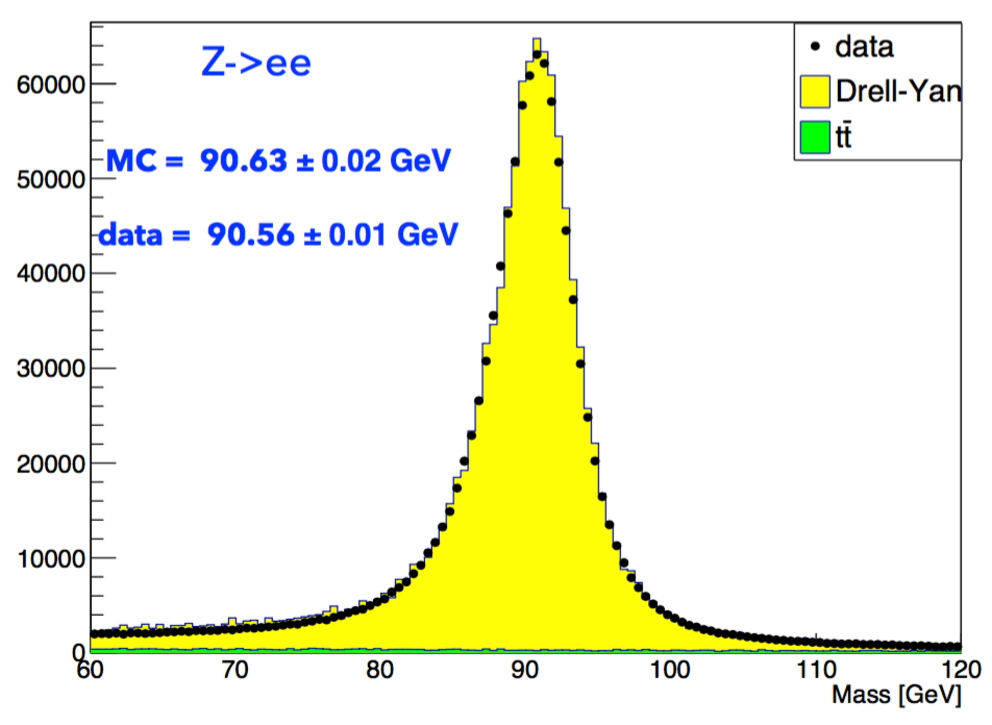
\includegraphics{Figures/Electrons/ele_energy_scale.pdf}}}
%\subfigure [] {\resizebox{9.5cm}{!}{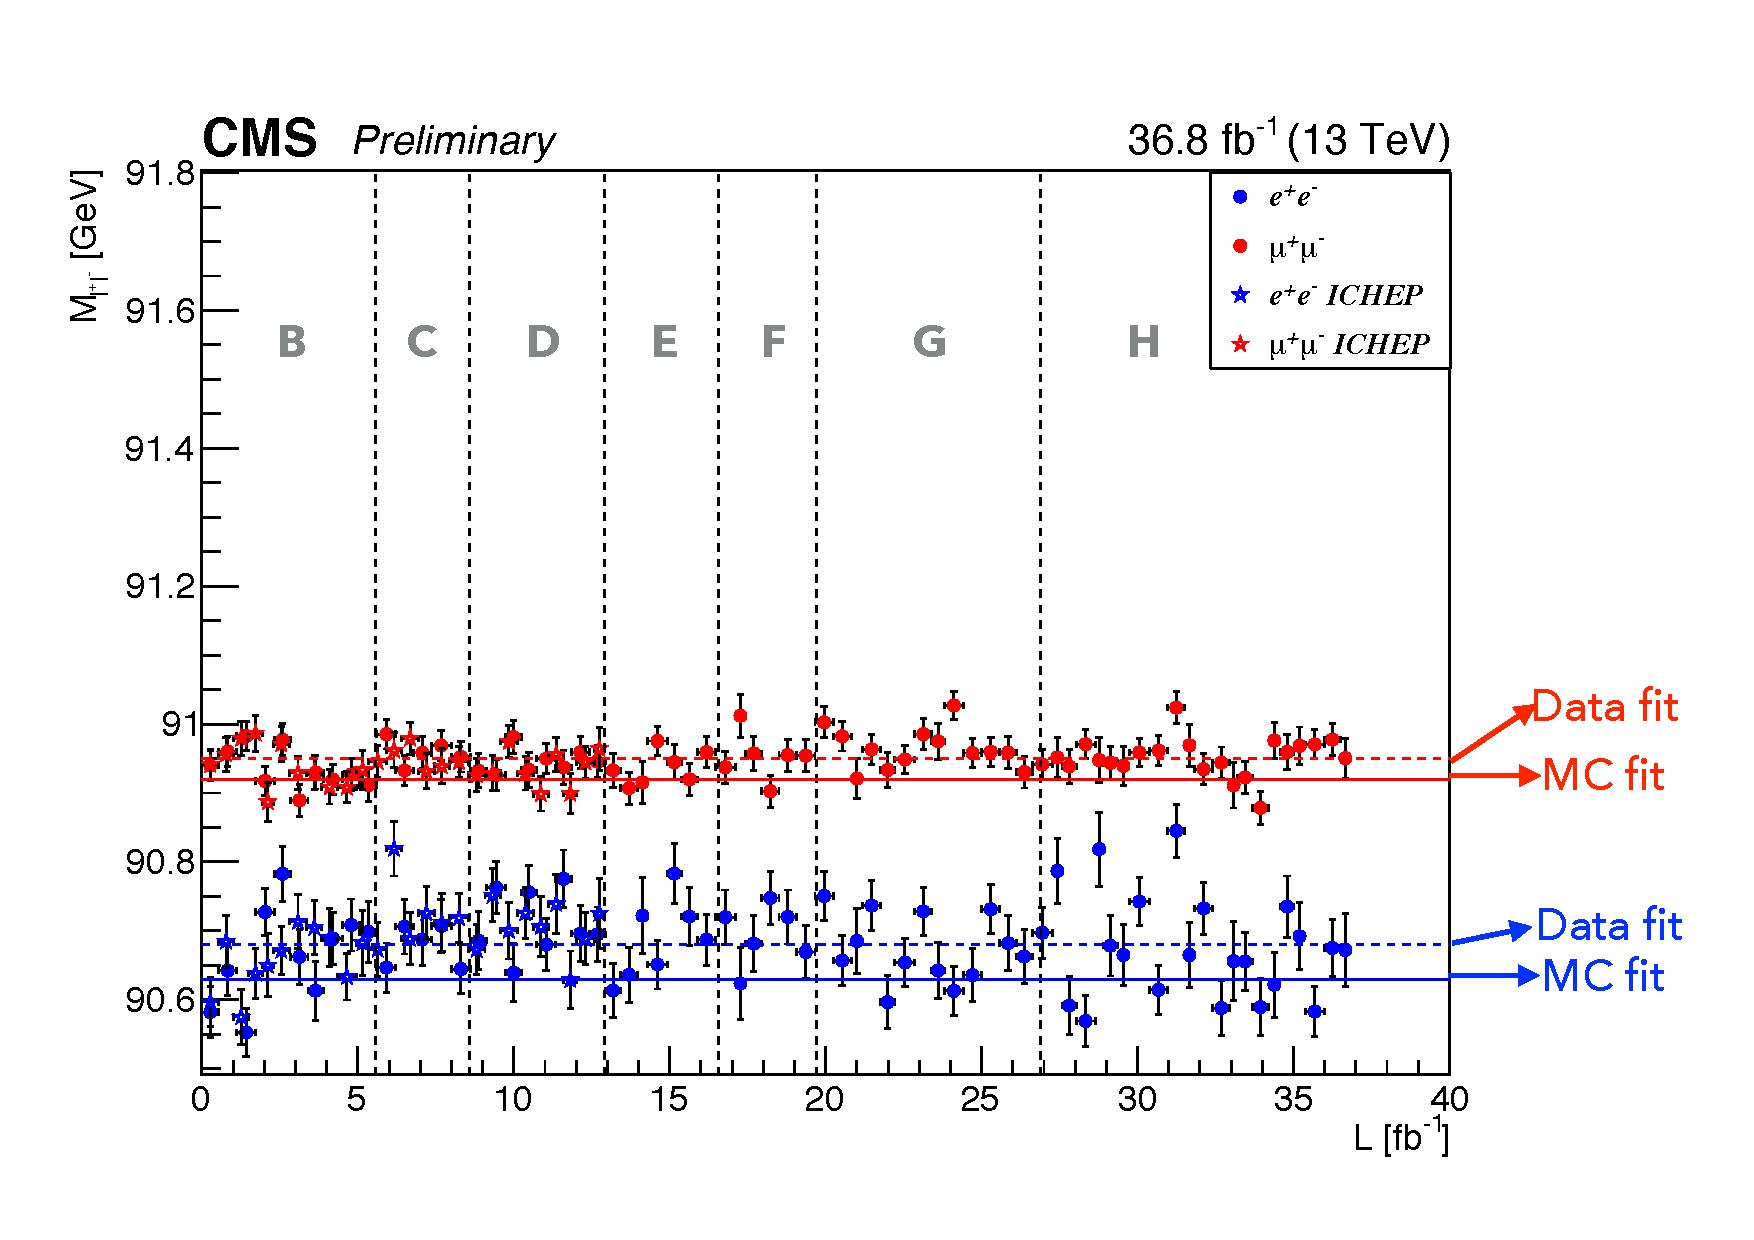
\includegraphics{Figures/Electrons/ele_energy_scale_per_lumi.pdf}}}
%\end{center}
%\caption{
%(a): electron energy scale measured in the $Z+\ell$ control region for EB and EE electrons. The results of the Crystall-ball fit are reported in the figure. 
%(b): lepton energy scales per 500~pb luminosity block. 
%}
%\label{fig:ele_energy_scale}
%\end{figure}

\begin{figure}[tbh]
\centering
\begin{subfigure}{0.45\textwidth}
\centering
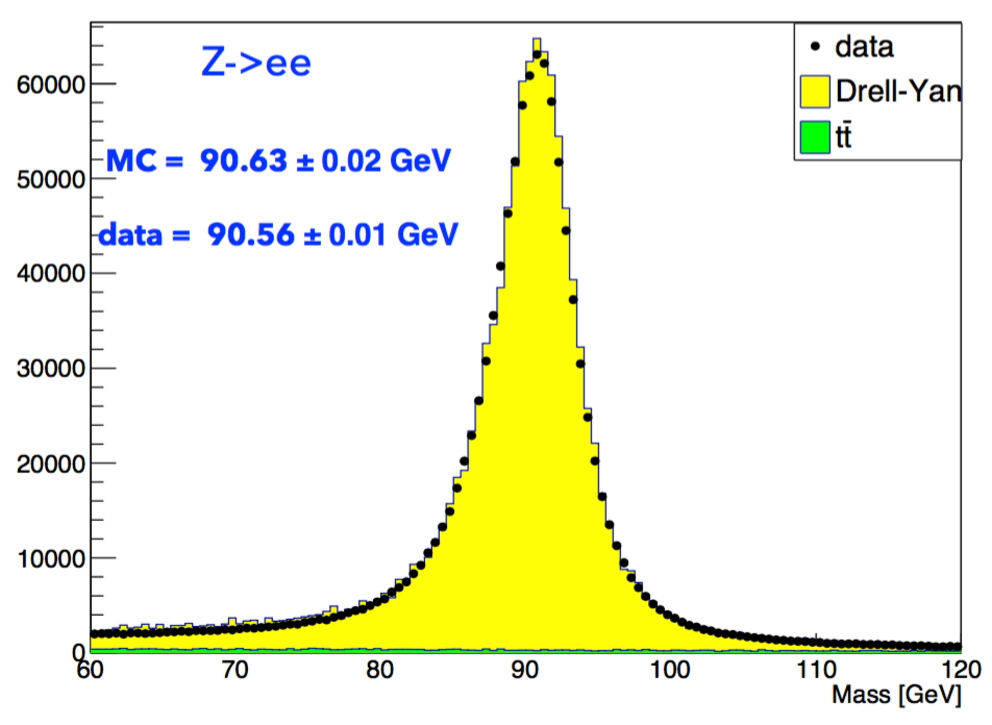
\includegraphics[width=2.5in]{Figures/Electrons/ele_energy_scale.pdf}
\caption{}
\end{subfigure}
\begin{subfigure}{0.45\textwidth}
\centering
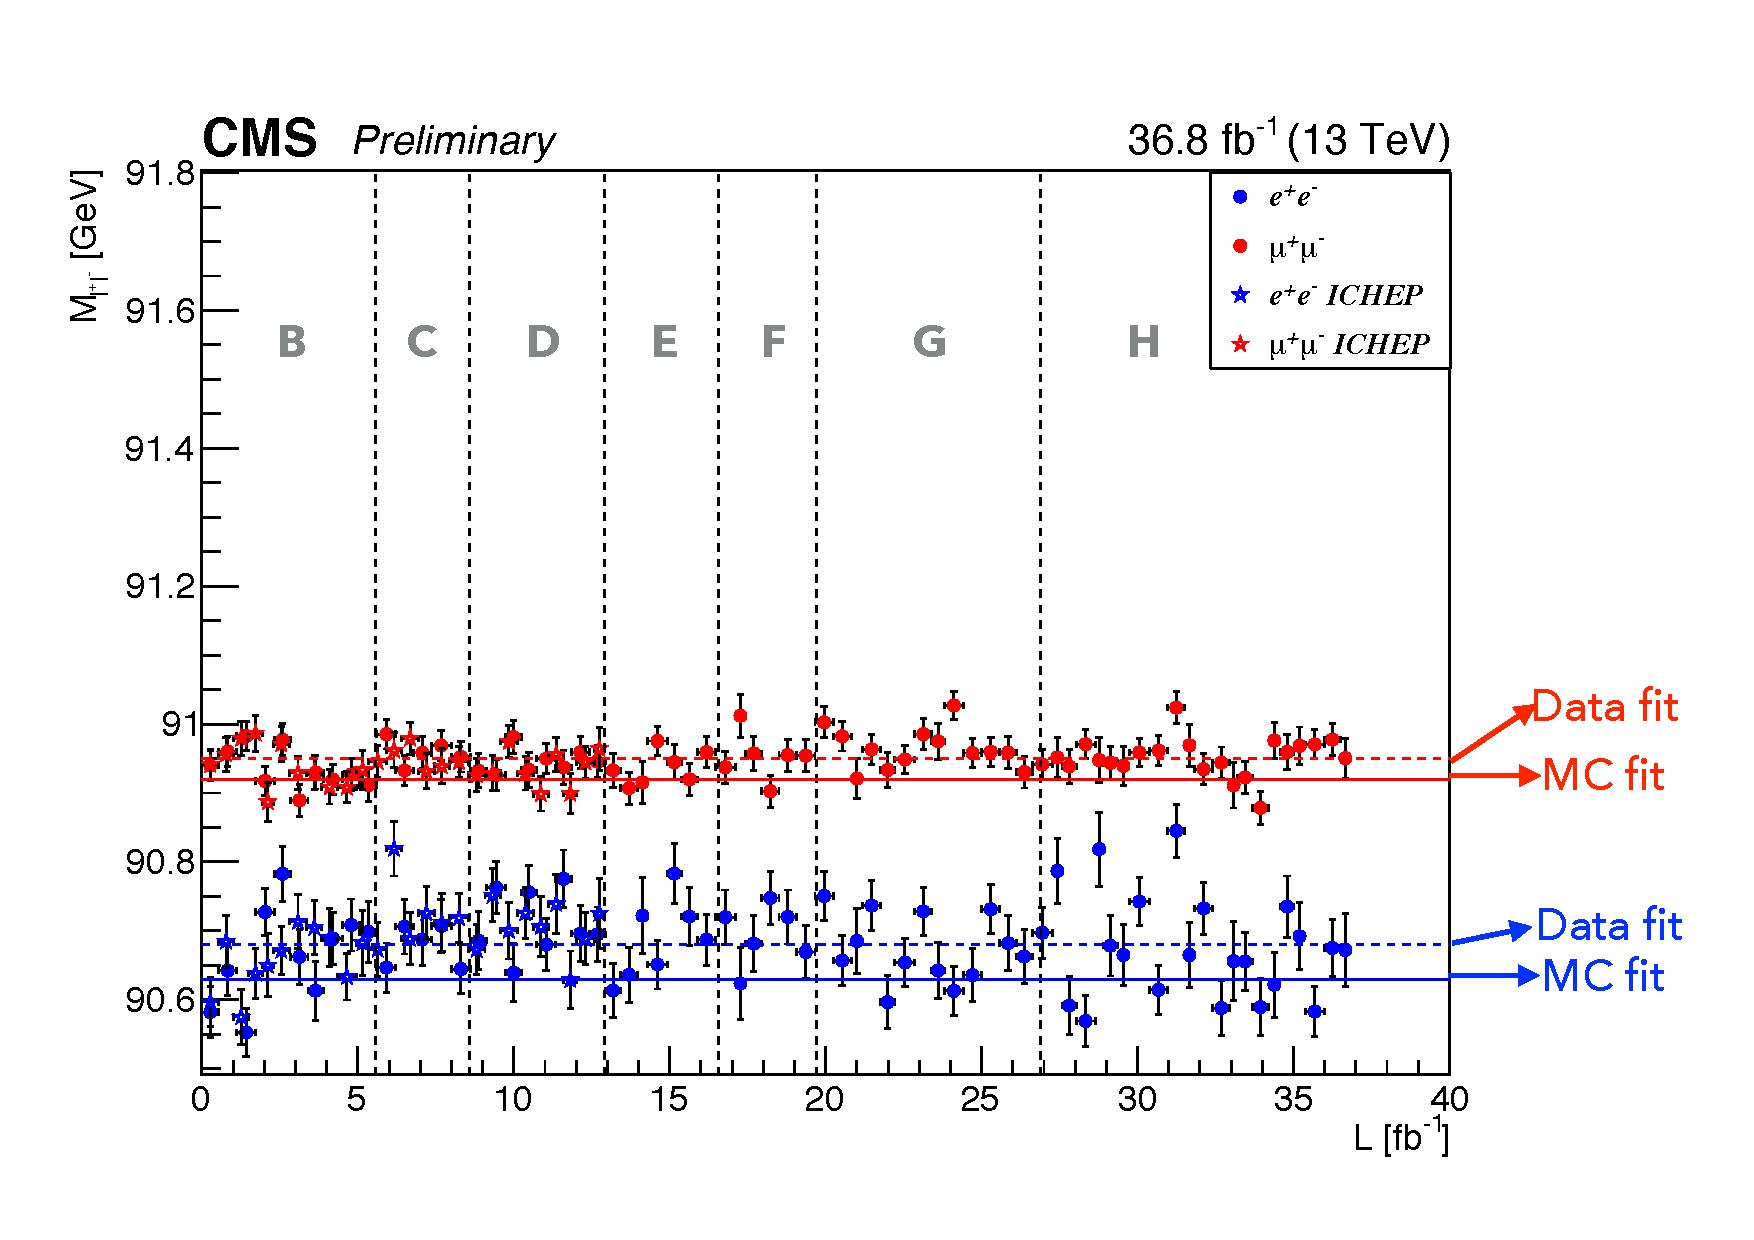
\includegraphics[width=2.5in]{Figures/Electrons/ele_energy_scale_per_lumi.pdf}
\caption{}
\end{subfigure}
\caption{(a): electron energy scale measured in the $Z+\ell$ control region for EB and EE electrons. The results of the Crystall-ball fit are reported in the figure. (b): lepton energy scales per 500~pb luminosity block.}
\label{fig:ele_energy_scale}
\end{figure}

\subsection{Electron Efficiency Measurements}
\label{sec:eleEffMeas}
%\input{Objects/eleEffMeas.tex}

The Tag-and-Probe study was performed on the single electron primary datasets listed in table \ref{tab:datasets_data} using the same golden JSON of 36.8 
fb$^{-1}$ as for the main analysis. More details on the Tag-and-Probe method can be found in Ref.~\cite{AN-15-277}. 

Tag electrons need to satisfy the following quality requirements:
\begin{itemize}
\item trigger matched to HLT\_Ele27\_eta2p1\_WPTight\_Gsf\_v*
\item $p_{T} > 30$~GeV, super cluster (SC) $\eta < 2.1$ but on in EB-EE gap ($1.4442<|\eta|<1.566$)
\item tight working point of the Spring16 cut-based electron ID
\end{itemize}

Probe electrons only need to be reconstructed as GsfElectron. The FSR recovery algorithm used in the main analysis is used consistently throughout the efficiency measurement: the isolations are calculated without any FSR photons matched to electrons and the probe electron \pt as well as the di-electron invariant mass include the FSR photons, if any. 


The nominal MC efficiencies are evaluated from the LO MadGraph Drell-Yan sample, while the NLO systematics use the 0,1 jet MadGraph\_AMCatNLO sample listed in Table \ref{tab:MCsamples}.

In contrast to previous efficiency measurements, a template fit is used here. The $m_{ee}$ signal shape of the passing and failing probes is taken from MC and convoluted with a Gaussian. The data is then fitted with the convoluted MC template and a CMSShape (an Error-function with a one-sided exponential tail). This change follows from the usage of the new T\&P tool developed by the EGM POG.


%\paragraph{Electron selection efficiency measurements}\mbox{}\\
%\label{par:Efficiency_measurements}

The electron selection efficiency is measured as a function of the probe electron $\pt$ and its SC $\eta$, and separately for electrons falling in the ECAL gaps. Figure \ref{fig:ele_sel_pt_turn_on} shows the $\pt$ turn-on curves measured in data, and the final 2D scale factor is shown in Fig.~\ref{fig:ele_sel_scale_factors} together with the systematic uncertainties. These scale factors are very similar to the ICHEP figures, but more homogenous across $\eta$ and $\pt$ because of the higher statistics and the usage of more stable fitting routines in the new T\&P tool.


%\begin{figure}[!htb]
%\begin{center}
%    \subfigure [] {\resizebox{7.5cm}{!}{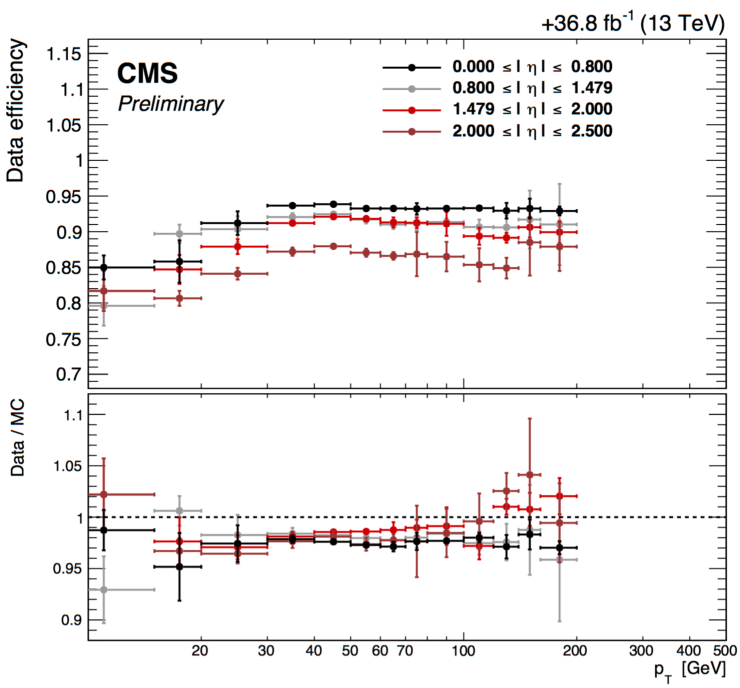
\includegraphics{Figures/Electrons/ele_eff_pt.pdf}}}
%    \subfigure [] {\resizebox{7.5cm}{!}{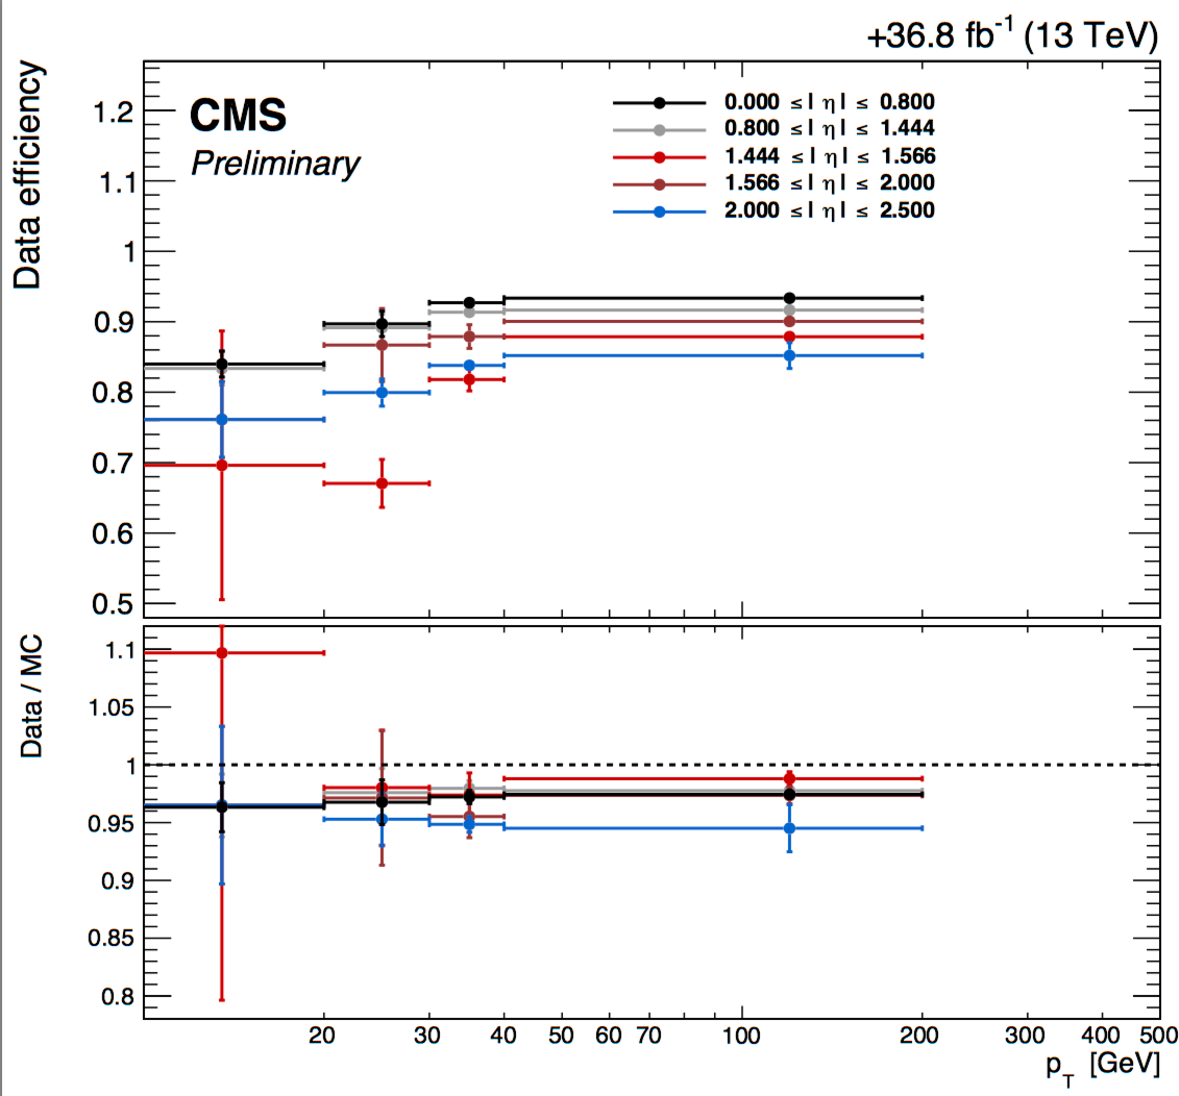
\includegraphics{Figures/Electrons/gap_ele_eff_pt.pdf}}}\\
%\caption{Electron selection efficiencies measured using the Tag-and-Probe technique described in the text, non-gap electrons (left) and gap electrons (right).}
%\label{fig:ele_sel_pt_turn_on}
%\end{center}
%\end{figure}

\begin{figure}[tbh]
\centering
\begin{subfigure}{0.45\textwidth}
\centering
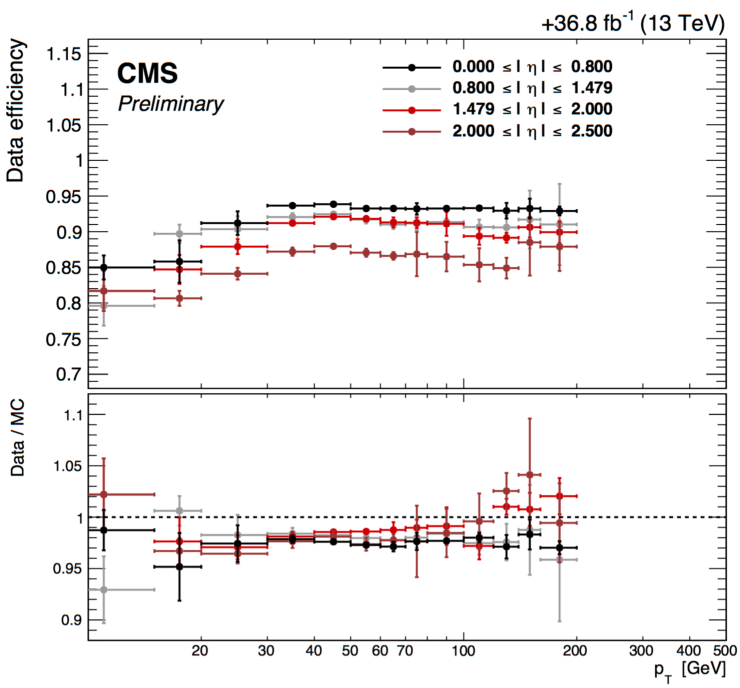
\includegraphics[width=2.2in]{Figures/Electrons/ele_eff_pt.pdf}
\caption{}
\end{subfigure}
\begin{subfigure}{0.45\textwidth}
\centering
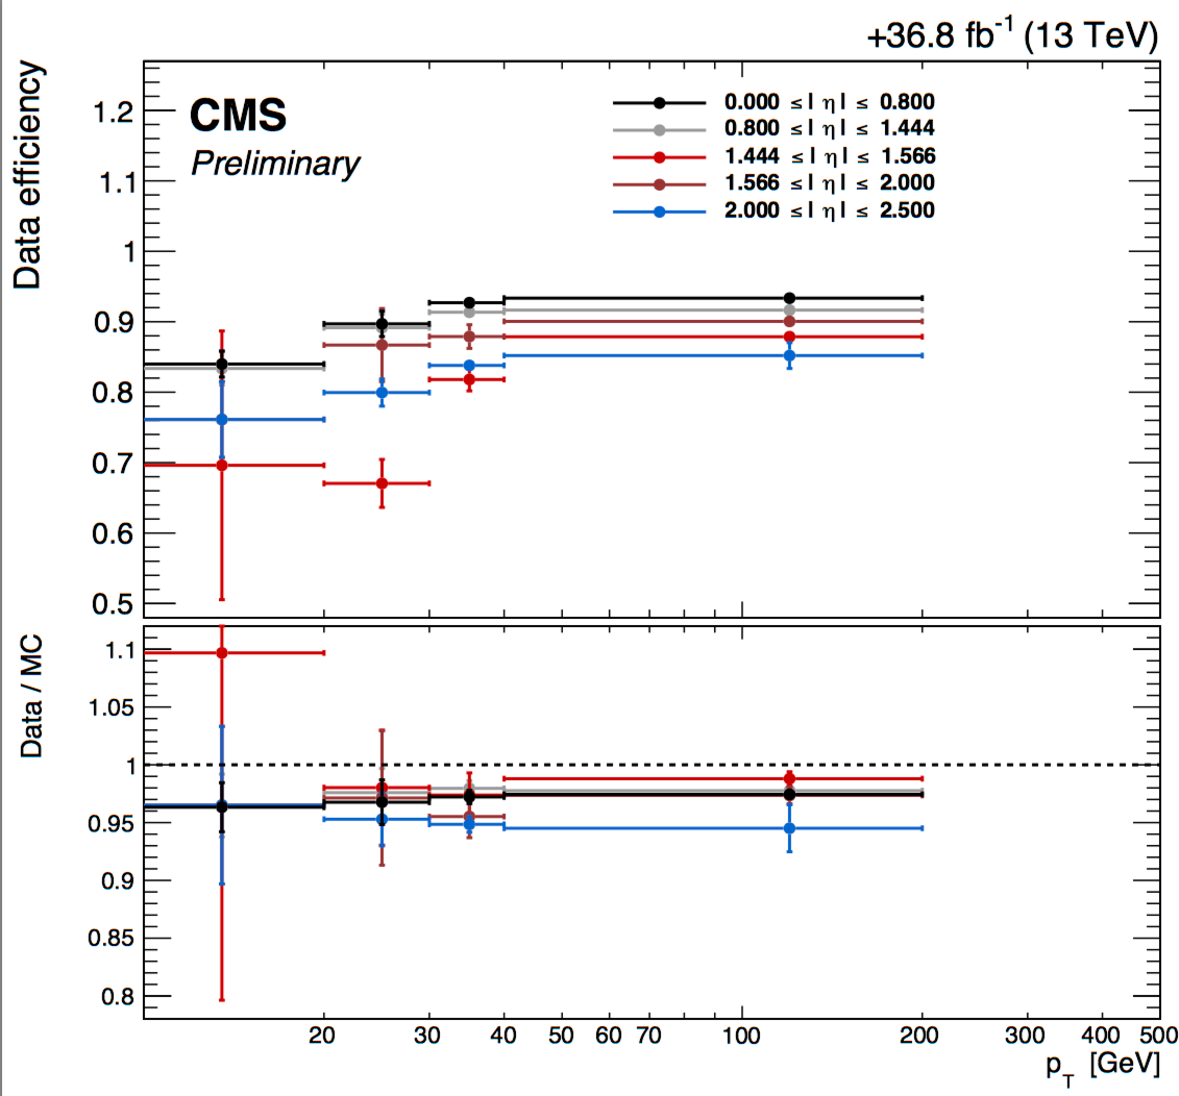
\includegraphics[width=2.2in]{Figures/Electrons/gap_ele_eff_pt.pdf}
\caption{}
\end{subfigure}
\caption{Electron selection efficiencies measured using the Tag-and-Probe technique described in the text, non-gap electrons (left) and gap electrons (right).}
\label{fig:ele_sel_pt_turn_on}
\end{figure}

%\begin{figure}[!htb]
%\begin{center}
%    \subfigure [] {\resizebox{15cm}{!}{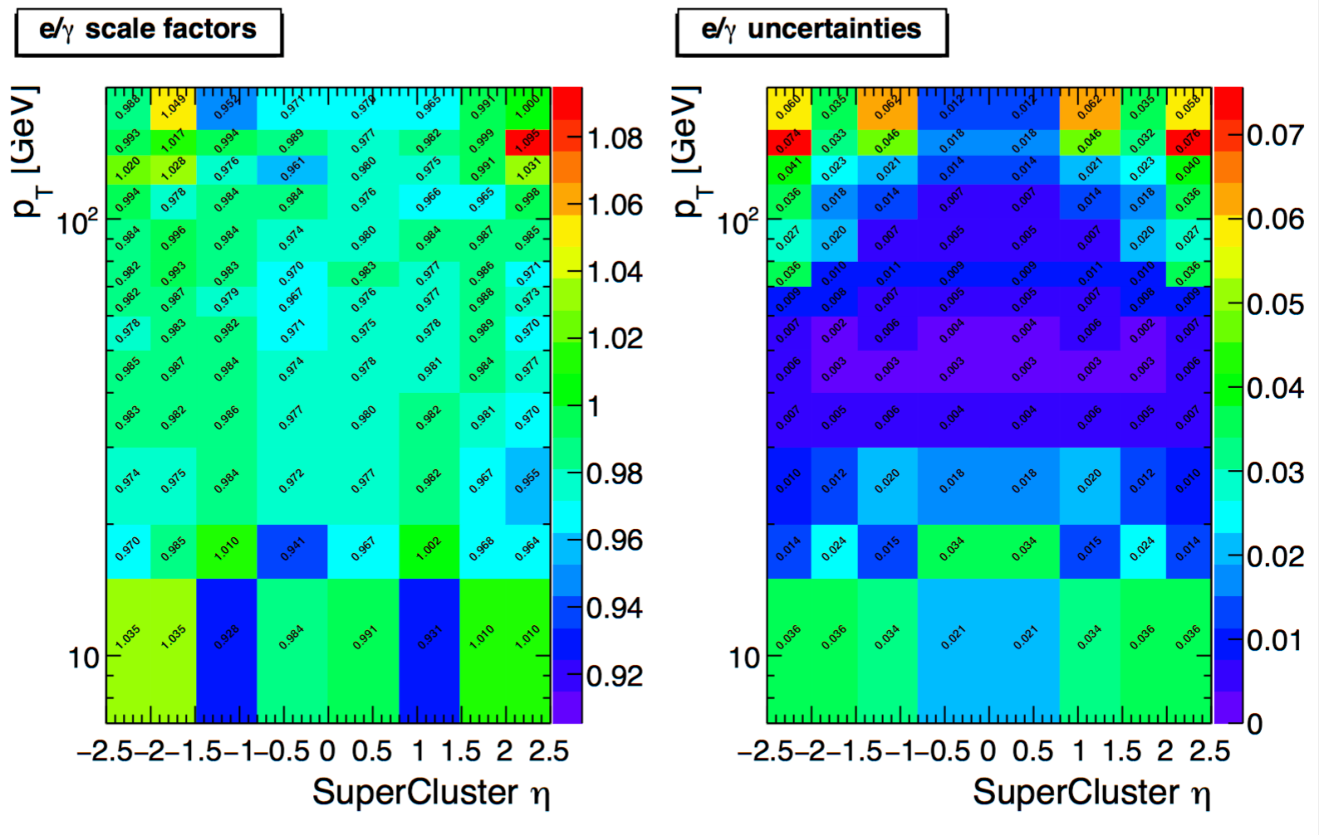
\includegraphics{Figures/Electrons/ele_eff_sf_unc.pdf}}}\\
%    \subfigure [] {\resizebox{15cm}{!}{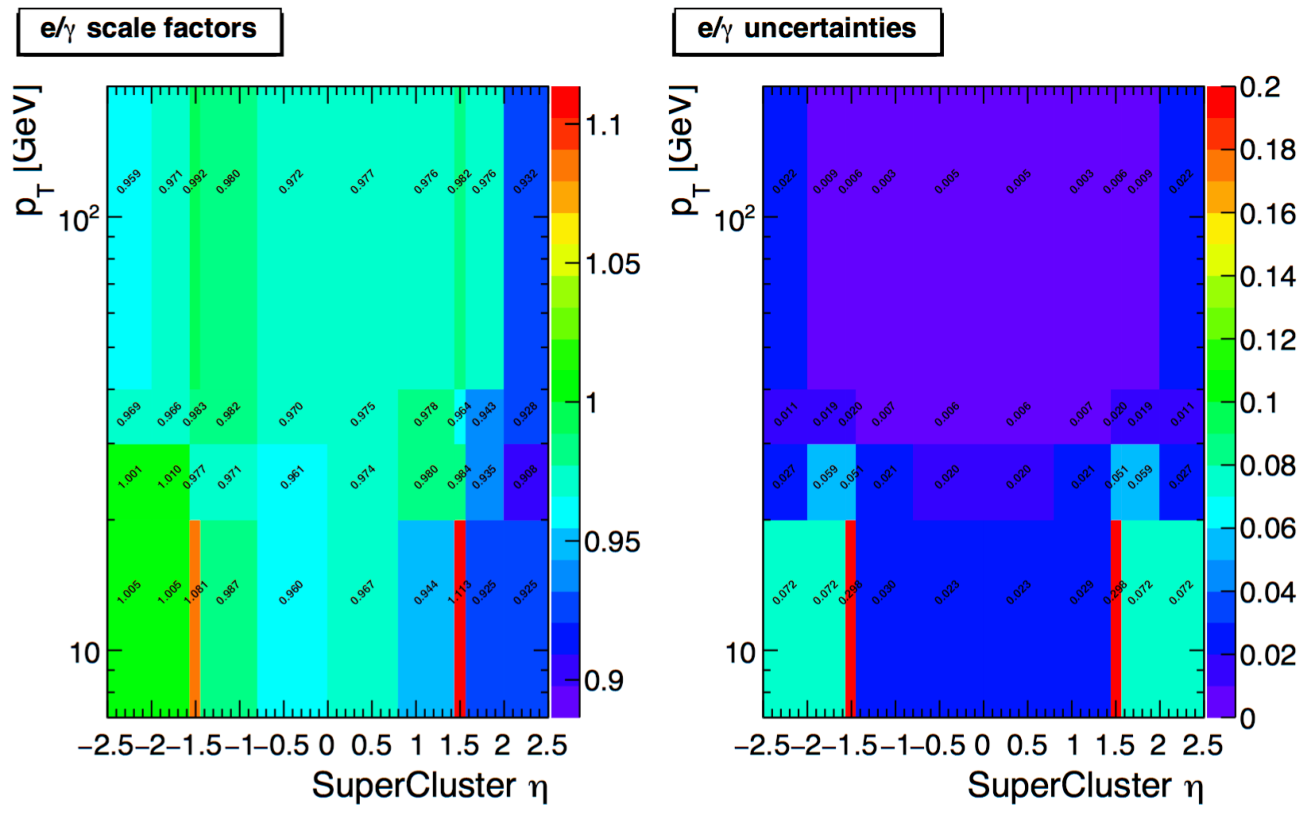
\includegraphics{Figures/Electrons/gap_ele_eff_sf_unc.pdf}}}
%\caption{Electron selection efficiencies measured using the Tag-and-Probe technique described in the text, non-gap electrons (top) and gap electrons (bottom).}
%\label{fig:ele_sel_scale_factors}
%\end{center}
%\end{figure}

\begin{figure}[tbh]
\centering
\begin{subfigure}{0.45\textwidth}
\centering
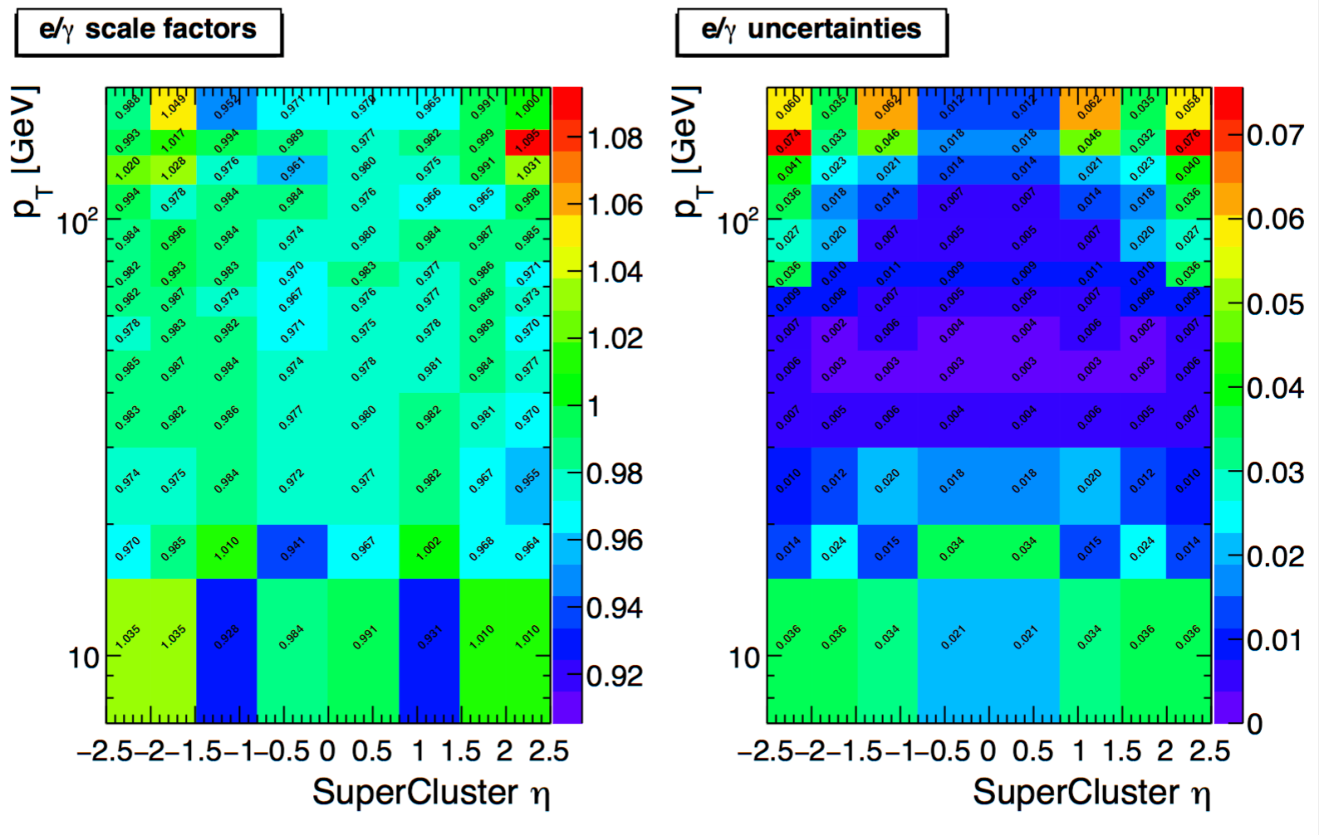
\includegraphics[width=2.5in]{Figures/Electrons/ele_eff_sf_unc.pdf}
\caption{}
\end{subfigure}
\begin{subfigure}{0.45\textwidth}
\centering
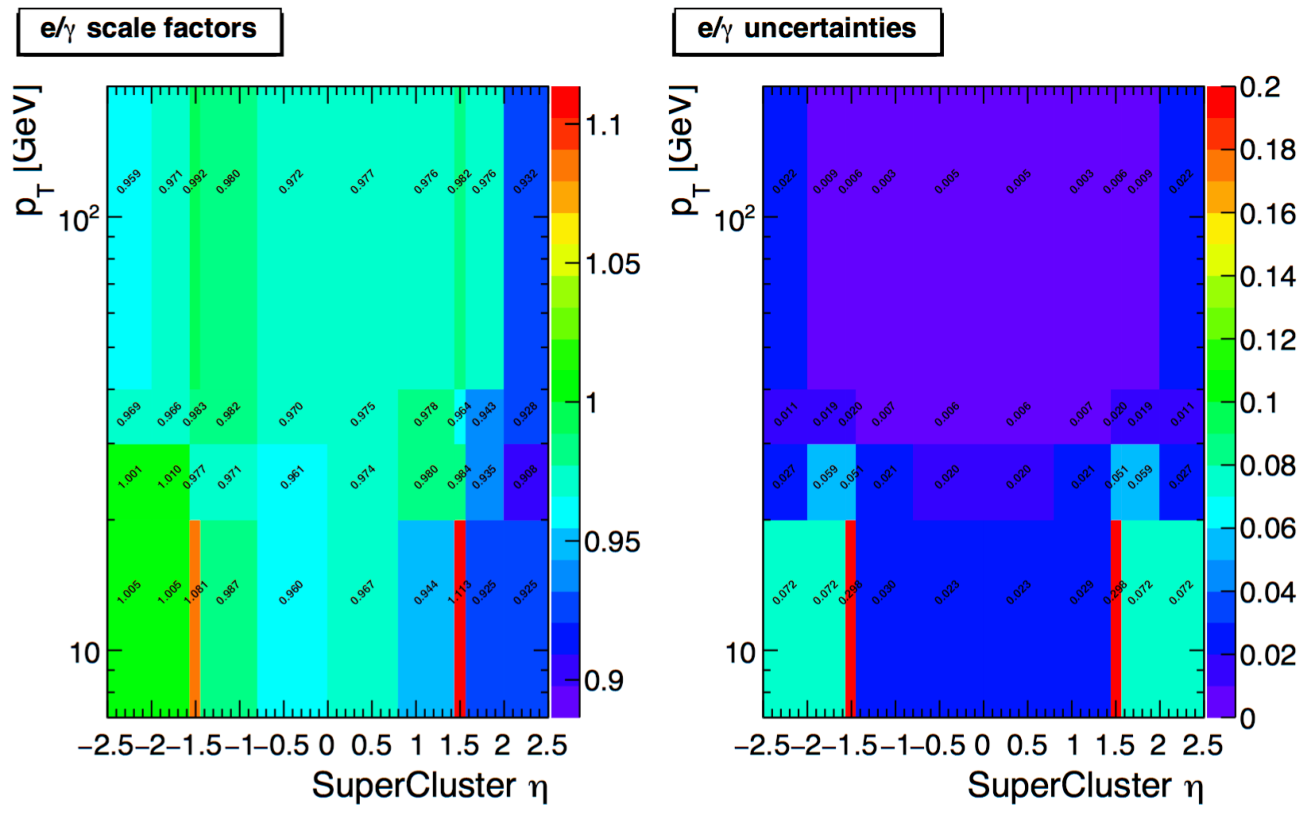
\includegraphics[width=2.5in]{Figures/Electrons/gap_ele_eff_sf_unc.pdf}
\caption{}
\end{subfigure}
\caption{Electron selection efficiencies measured using the Tag-and-Probe technique described in the text, non-gap electrons (top) and gap electrons (bottom)}
\label{fig:ele_sel_scale_factors}
\end{figure}


%\paragraph{Systematic uncertainties}\mbox{}\\
%\label{par:Systematic_uncertainties}
%%%%%%%%%%%%%%%%%%%%%%%%%%%%

 The EGM recommendations on the evaluation of Tag-and-Probe uncertainties for efficiency measurements are followed. Specifically,

\begin{itemize}
   \item Variation of the signal shape from a MC shape to an analytic shape (Crystal Ball) fitted to the MC
   \item Variation of the background shape from a CMS-shape to a simple exponential in fits to data
   \item Variation of the tag selection: tag $p_{T}>$35~GeV and passes MVA-based 8X ID
   \item Using an NLO MC sample for the signal templates
\end{itemize}

The total uncertainty for the measurement of the scale factors is the quadratic sum of the statistical uncertainties returned from the fit and the aforementioned systematic uncertainties.


\section{Muons}

\subsection{Muon Reconstruction and Identification}
\label{sec:muonReco}

More details on muon reconstruction can be found in Ref.~\cite{AN-15-277}.
We define {\bf loose muons} as the muons that satisfy  
$p_T > 5$, $|\eta| < 2.4$, $d_{xy}< 0.5$, $d_z < 1$, where $d_{xy}$ and $d_z$ are 
defined w.r.t. the PV and using the 'muonBestTrack'. Muons have to be 
reconstructed by either the Global Muon or Tracker Muon algorithm. Standalone 
Muon tracks that are only reconstructed in the muon system are rejected.
Muons with \verb|muonBestTrackType==2| (standalone) are discarded even if they 
are marked as global or tracker muons. 

Loose muons with $\pt$ below 200\GeV are considered {\bf tight muons} if they 
also pass the PF muon ID (note that the naming 
convention used for these IDs differs from the muon POG naming scheme, in which
the ``tight ID'' used here is called the ``loose ID''). Loose muons with $\pt$ 
above 200\GeV are considered tight muons if they pass the PF ID or the Tracker
High-$\pt$ ID, the definition of which is shown in Table~\ref{tab:highPtID}.
This relaxed definition is used to increase signal efficiency for the high-mass
search. When a very heavy resonance decays to two $\cPZ$ bosons, both bosons
will be very boosted. In the lab frame, the leptons coming from the decay of
a highly boosted $\cPZ$ will be nearly collinear, and the PF ID loses 
efficiency for muons separated by approximately $\Delta R < 0.4$, which roughly 
corresponds to muons originating from $\cPZ$ bosons with $\pt > 500\GeV$.

\begin{table}[h]
    \begin{small}
    \begin{center}
    \begin{tabular}{|l|l|}
      \hline
      Plain-text description         & Technical description                 \\
      \hline
      Muon station matching          & Muon is matched to segments           \\
                                     & in at least two muon stations         \\
                                     & \textbf{NB: this implies the muon is} \\
                                     & \textbf{an arbitrated tracker muon.}  \\
      \hline                                                          
      Good $\pt$ measurement         & $\frac{\pt}{\sigma_{\pt}} < 0.3$      \\
      \hline
      Vertex compatibility ($x-y$)   & $d_{xy} < 2$~mm                       \\
      \hline
      Vertex compatibility ($z$)     & $d_{z} < 5$~mm                        \\
      \hline
      Pixel hits                     & At least one pixel hit                \\
      \hline
      Tracker hits                   & Hits in at least six tracker layers   \\
      \hline
    \end{tabular}
    \caption{
      The requirements for a muon to pass the Tracker High-$\pt$ ID. Note that
      these are equivalent to the Muon POG High-$\pt$ ID with the global track 
      requirements removed.
      }
    \label{tab:highPtID}
    \end{center}
    \end{small}
\end{table}

An additional ``ghost-cleaning'' step is performed to deal with situations when a single muon
can be incorrectly reconstructed as two or more muons:

\begin{itemize}

\item Tracker Muons that are not Global Muons are required to be arbitrated.
\item If two muons are sharing 50\% or more of their segments then the muon with lower quality is removed.

\end{itemize}

\subsection{Muon Isolation}
\label{sec:muoniso}

Particle-Flow based isolation, described for electrons in section~\ref{sec:eleiso}, is also used for the muons. 
The only difference with electrons is the way the pileup contribution is subtracted: for the muons, $\Delta\beta$ correction is applied, whereby $\Delta\beta = \frac{1}{2} \sum^\text{charged had.}_\text{PU} \pt$  gives an estimate of the energy deposit of neutral particles (hadrons and photons) from pile-up vertices. 
The relative isolation for muons is then defined as:
\begin{equation}
\text{RelPFiso} = \frac{\sum^\text{charged had.} \pt + \max(\sum^\text{neutral had.} \ET 
+ \sum^\text{photon} \ET - \Delta \beta, 0)}{\pt^\text{lepton}}
\label{eqn:mupfiso}
\end{equation}

The isolation working point for muons was optimized in Ref.~\cite{AN-15-277} and the working point was chosen to be the same as electrons,
namely $\text{RelPFiso}(\Delta R = 0.3) < 0.35$. 


%\subsection{Muon Energy Calibrations}
% \input{Objects/muCalib}

\subsection{Muon Efficiency Measurements}
\label{sec:muonEffMeas}

Muon efficiencies are measured with the Tag and Probe (T\&P) method performed on
$\cPZ \to \Pgm\Pgm$ and $\JPsi\to\mu\mu$ events in bins of $\pt$ and $\eta$. More
details on the methodology can be found in Ref.~\cite{AN-15-277}.
%
The $\Z$ sample is used to measure the muon reconstruction and identification efficiency at high $\pt$,
and the efficiency of the isolation and impact parameter requirements at all $\pt$.
%
The $\JPsi$ sample is used to measure the reconstruction efficiency at low $\pt$,
as it benefits from a better purity in that kinematic regime. In this case,
events are collected using \verb=HLT_Mu7p5_Track2_Jpsi_v*= when probing the
reconstruction and identification efficiency in the muon system, and using the
 \verb=HLT_Mu7p5_L2Mu2_Jpsi_v*= when probing the tracking efficiency.

\paragraph*{Reconstruction and identification}

Results for the muon reconstruction and identification efficiency for $\pt > 20\GeV$
have been derived by the Muon POG.
The probe in this measurement are tracks reconstructed in the inner tracker, and
the passing probes are those that are also reconstructed as a global or tracker muon 
and passing the Muon POG Loose muon identification.
%
Results for low $\pt$ muons were derived using \JPsi events, with the same definitions
of probe and passing probes. The systematic uncertainties are estimated by varying the analytical signal and background shape models used to fit 
the dimuon invariant mass. Details on the procedure can be found in Ref.~\cite{AN-15-277}. The efficiency and scale 
factors used for low $\pt$ muons are the ones derived using single muon prompt-reco dataset.

The efficiency in data and simulation is shown in Fig.~\ref{fig:MuonIDEff_1}. 


\begin{figure}[tbh]
\centering
\begin{subfigure}{0.25\textwidth}
\centering
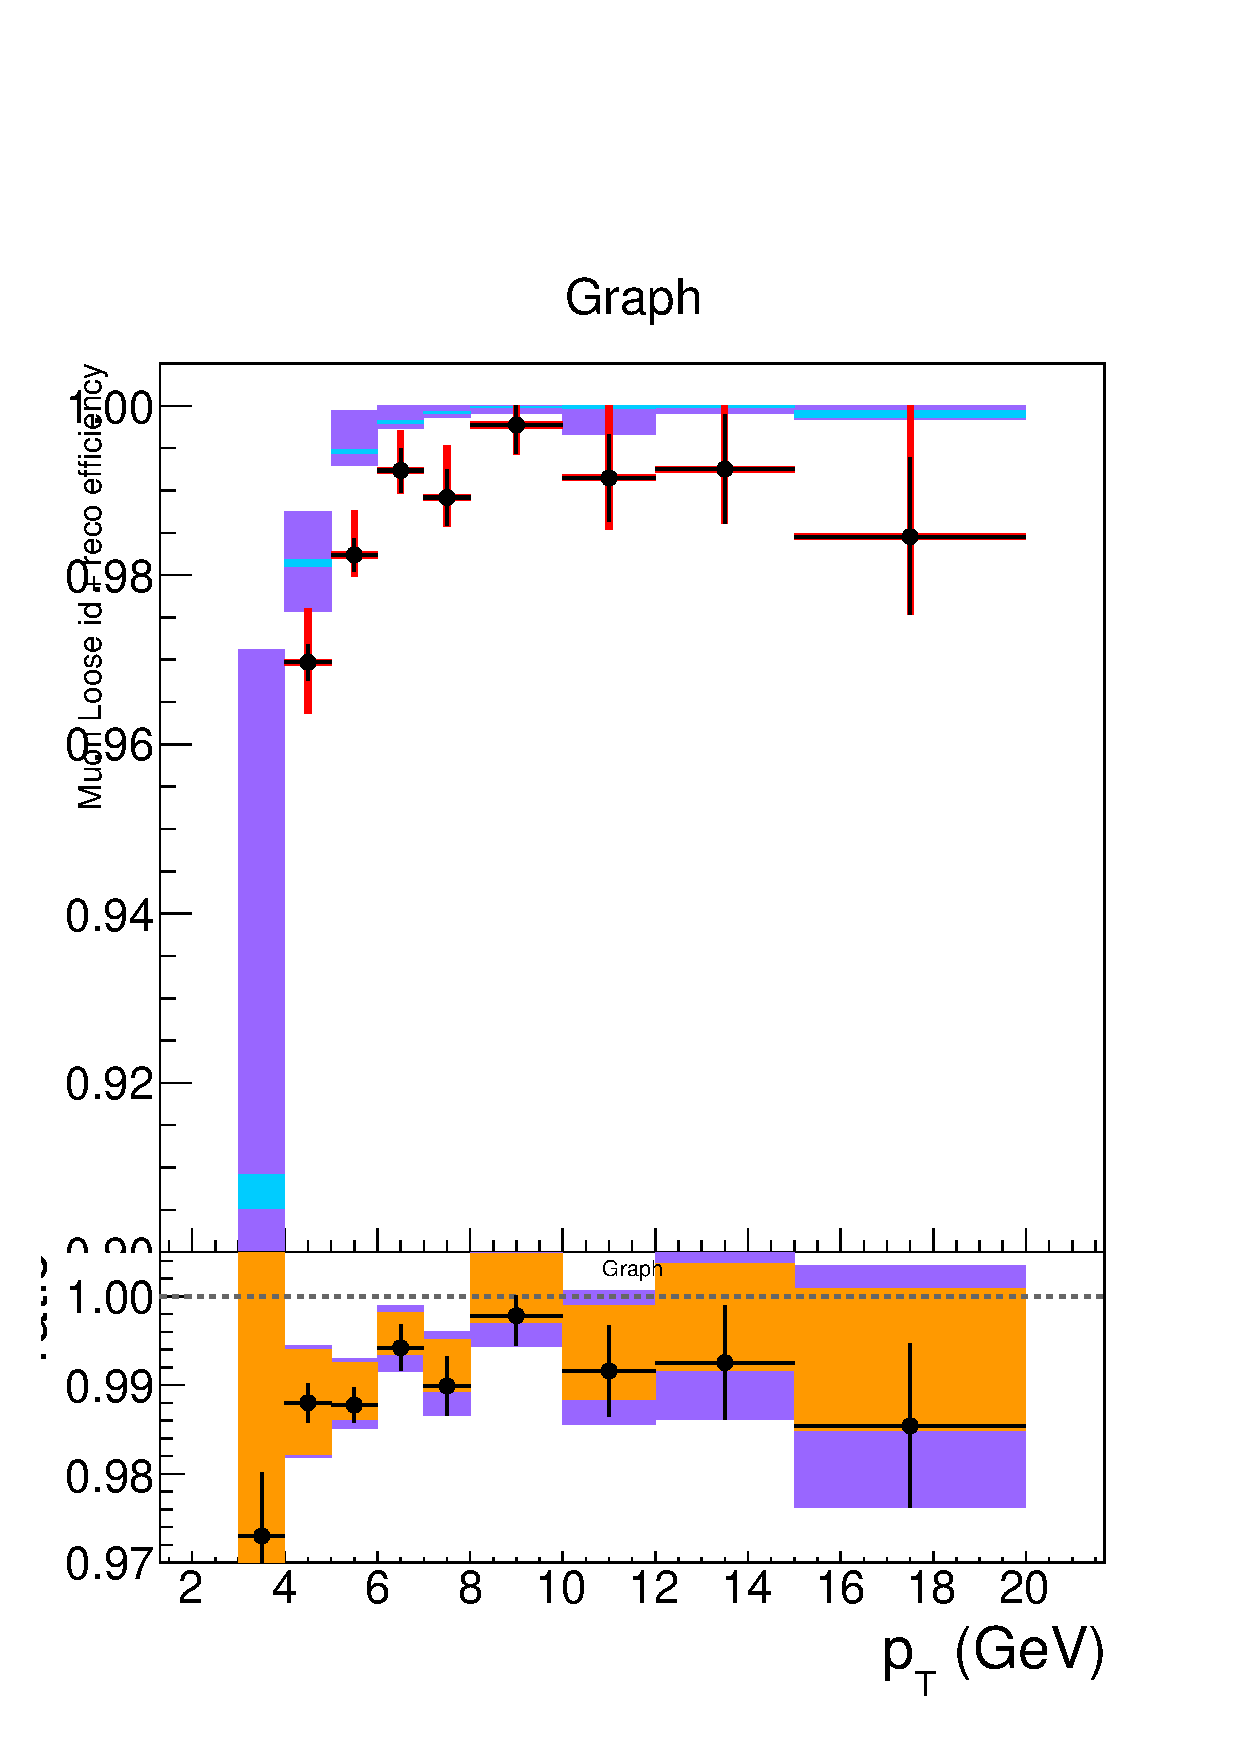
\includegraphics[width=1.5in]{Figures/Muons/mu_Loose_barrel.pdf}
\caption{}
\end{subfigure}
\begin{subfigure}{0.25\textwidth}
\centering
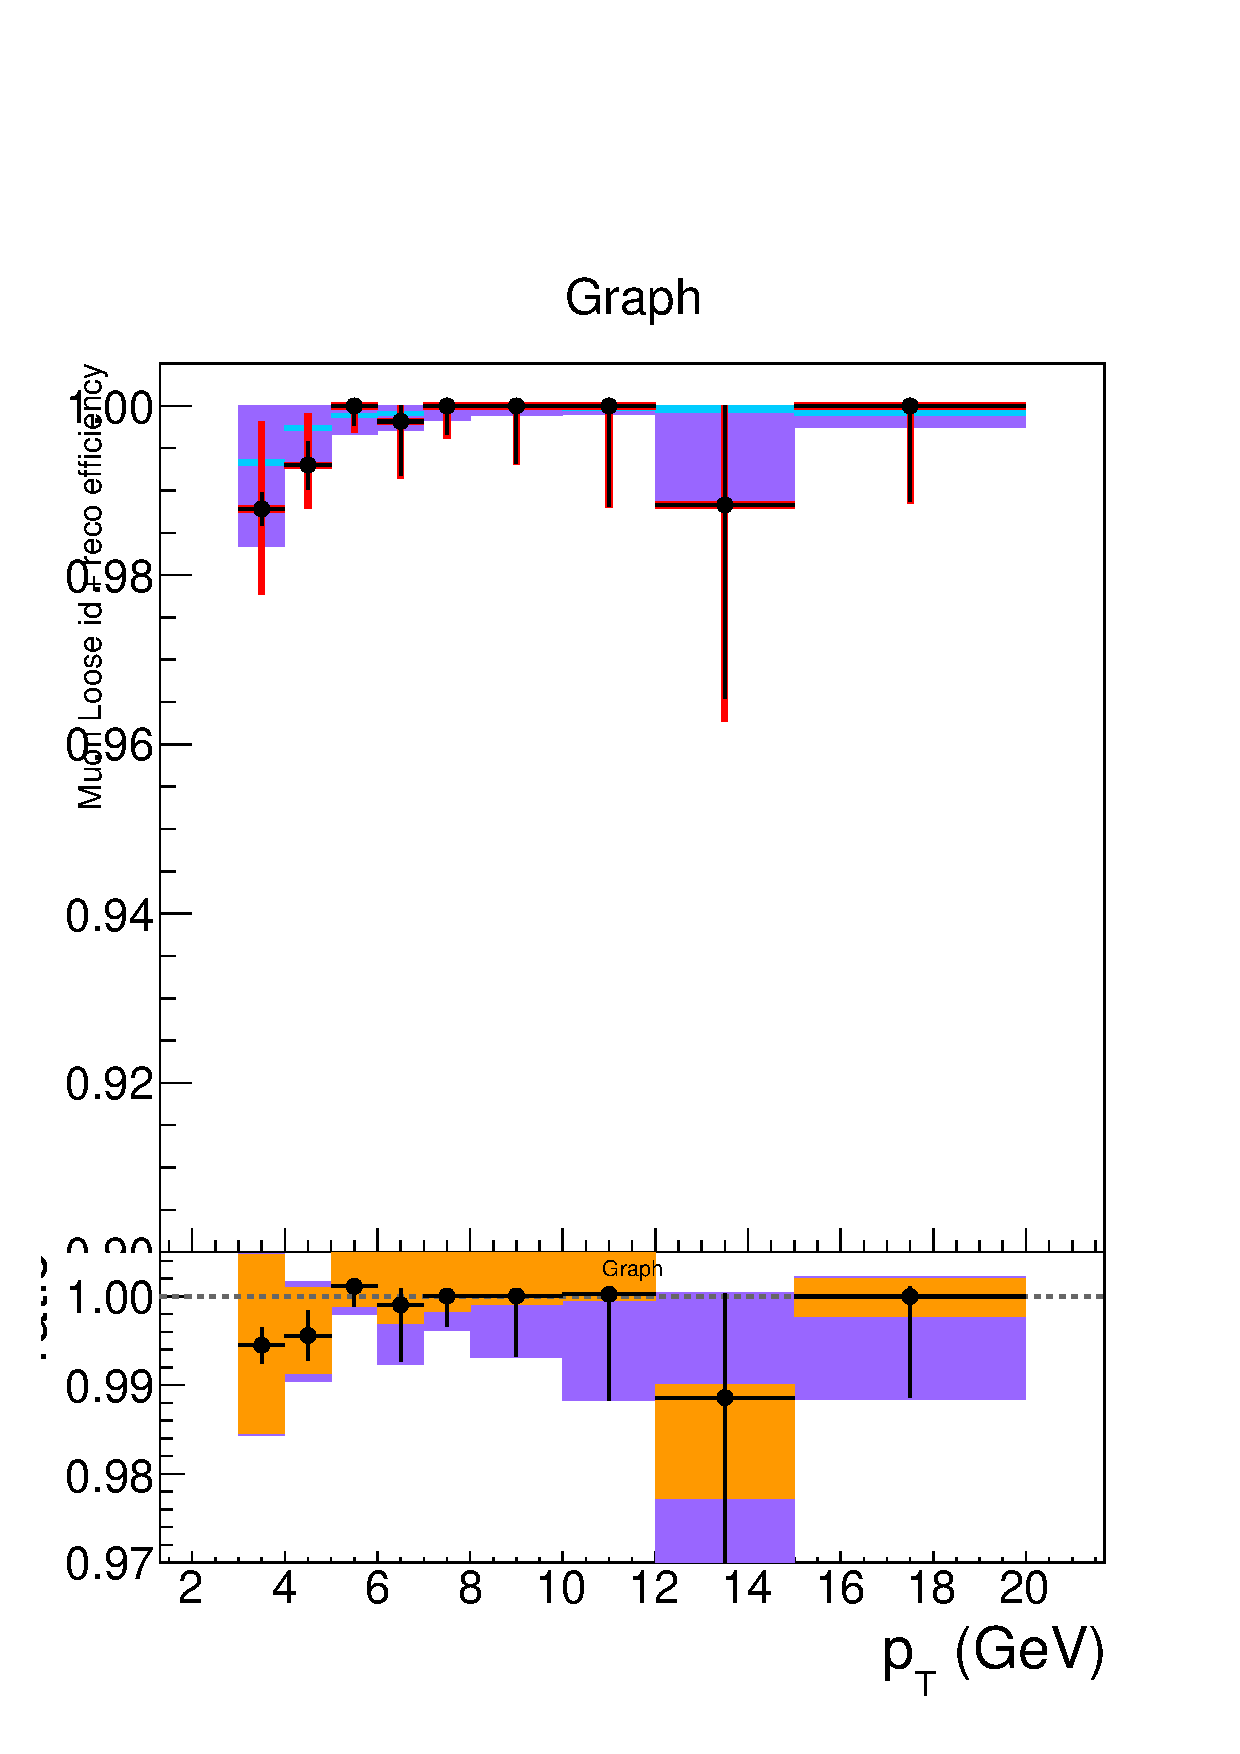
\includegraphics[width=1.5in]{Figures/Muons/mu_Loose_endcap.pdf}
\caption{}
\end{subfigure}
\begin{subfigure}{0.25\textwidth}
\centering
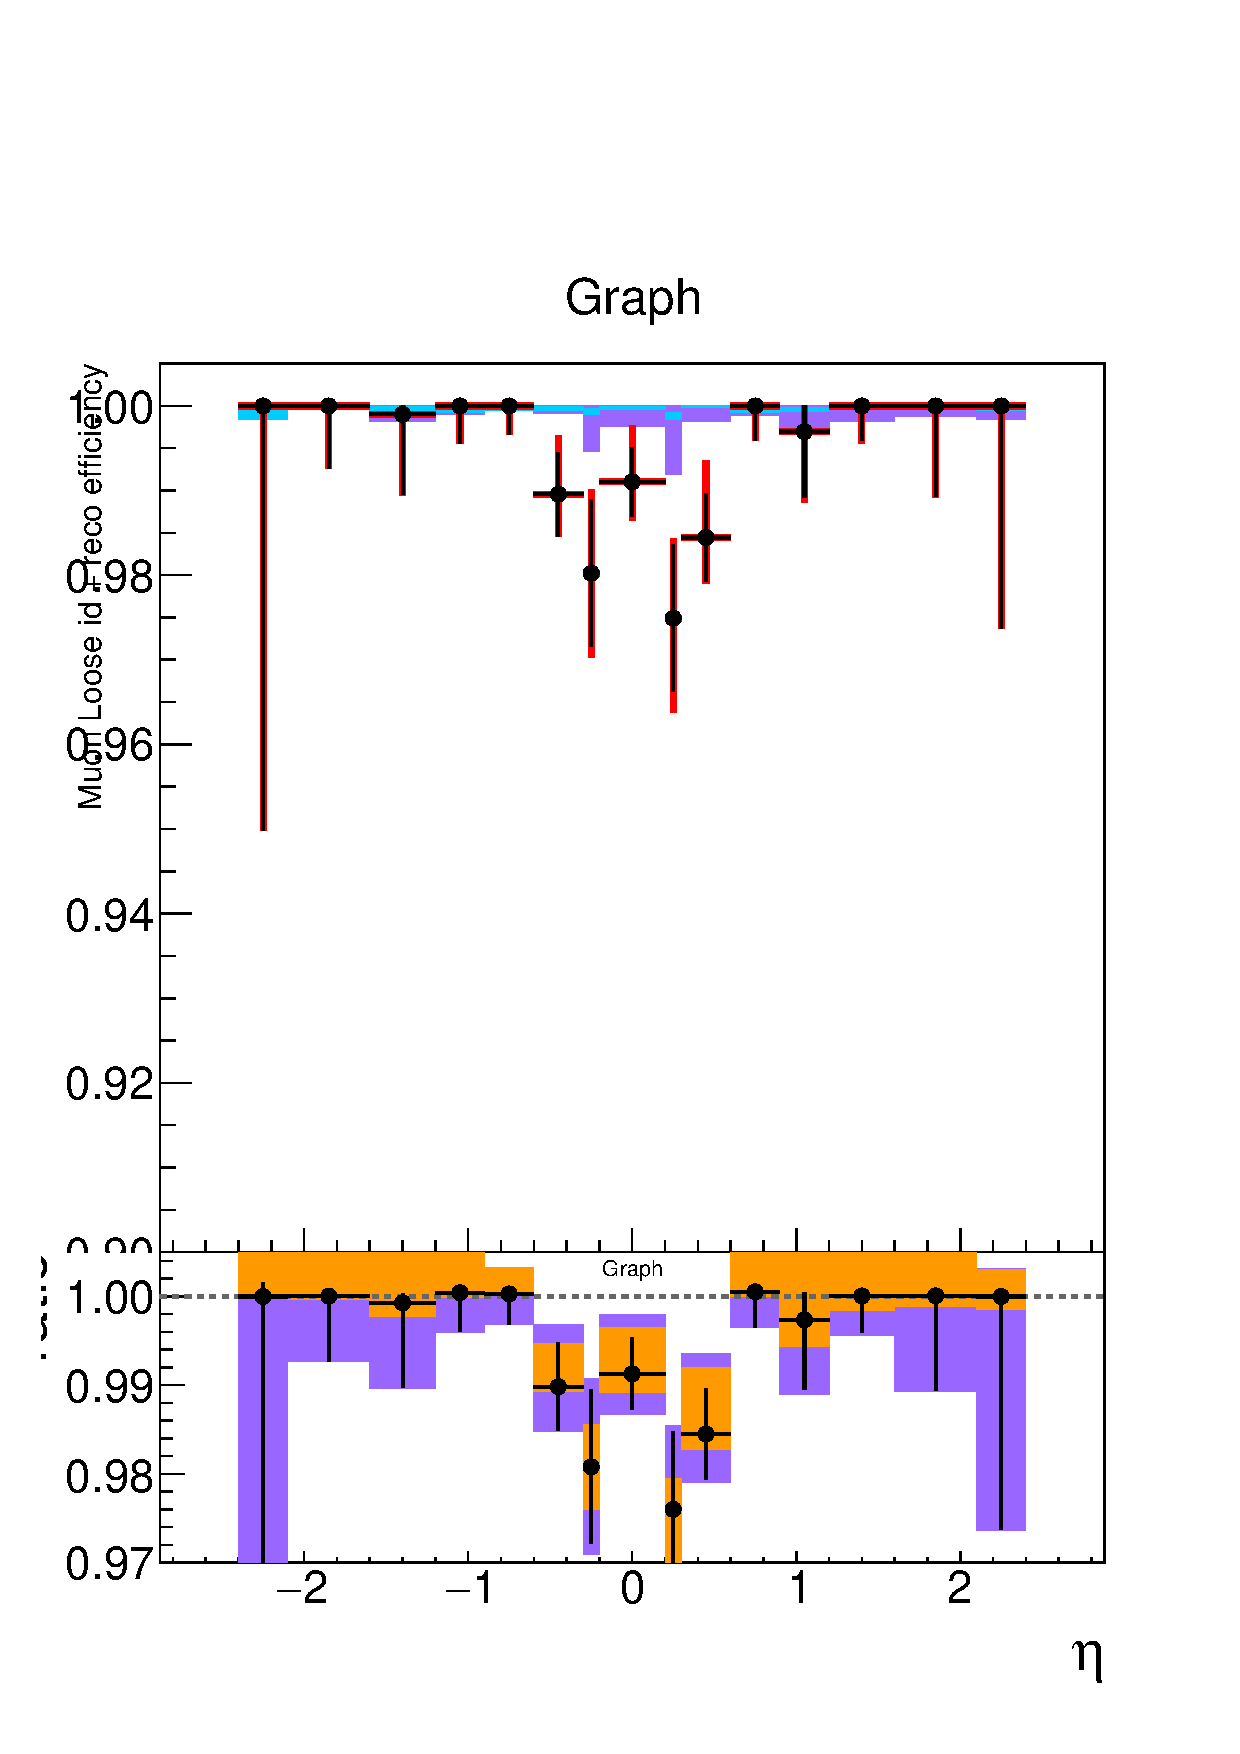
\includegraphics[width=1.5in]{Figures/Muons/mu_Loose_pt7.pdf}
\caption{}
\end{subfigure}
    \caption{Muon reconstruction and identification efficiency at low \pt, measured with the tag\&probe method on \JPsi events, as function of \pt in the barrel (left) and endcaps (center), and as function of $\eta$ for $\pt > 7\GeV$ (right). In the upper panel, the larger error bars include also the systematical uncertainties, while the smaller ones are purely statistical. In the lower panel showing the ratio of the two efficiencies, the black error bars are for the statistical uncertainty, the orange rectangles for the systematical uncertainty and the violet rectangles include both uncertainties.}
\label{fig:MuonIDEff_1}
\end{figure}

%\begin{figure}[htbp]
%  \begin{center}
%    \subfigure[]{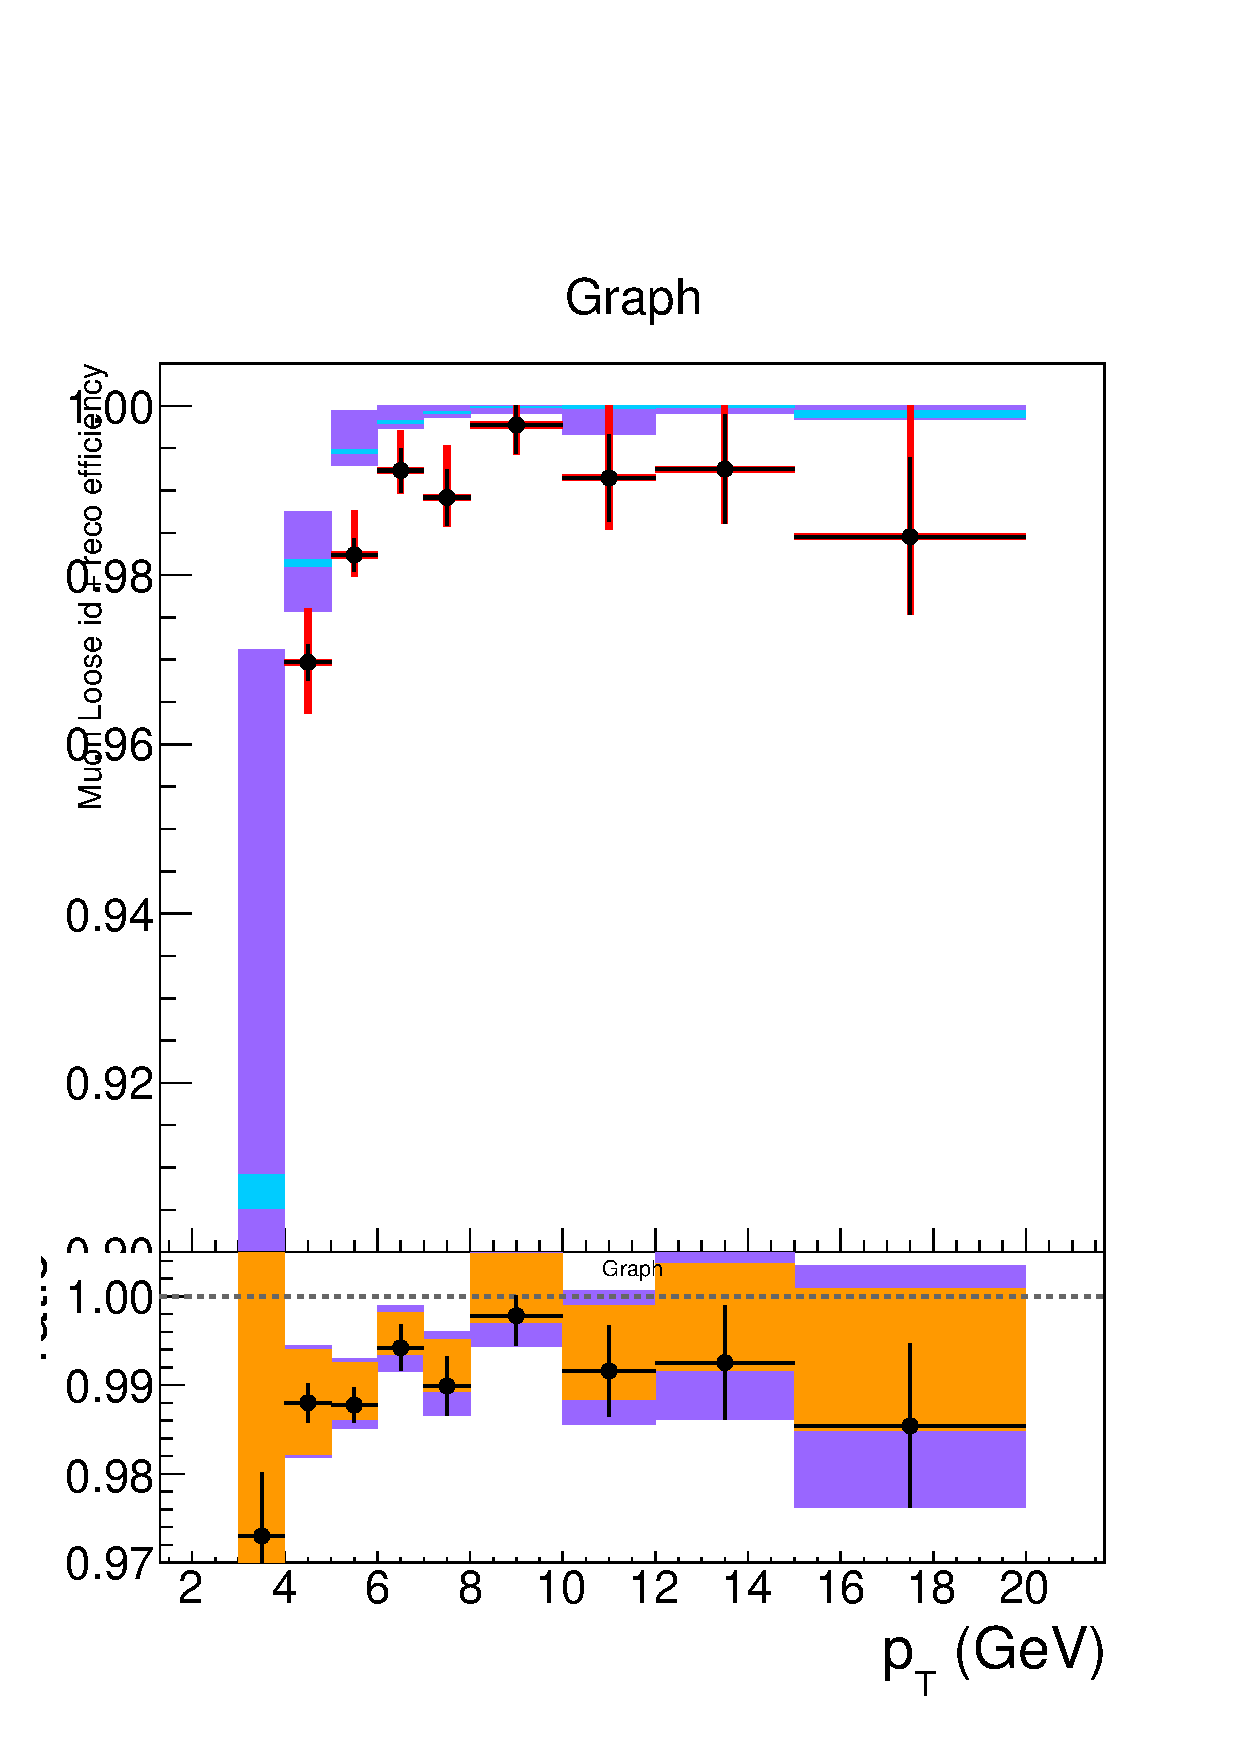
\includegraphics[width=0.32\textwidth]{Figures/Muons/mu_Loose_barrel.pdf}}
%    \subfigure[]{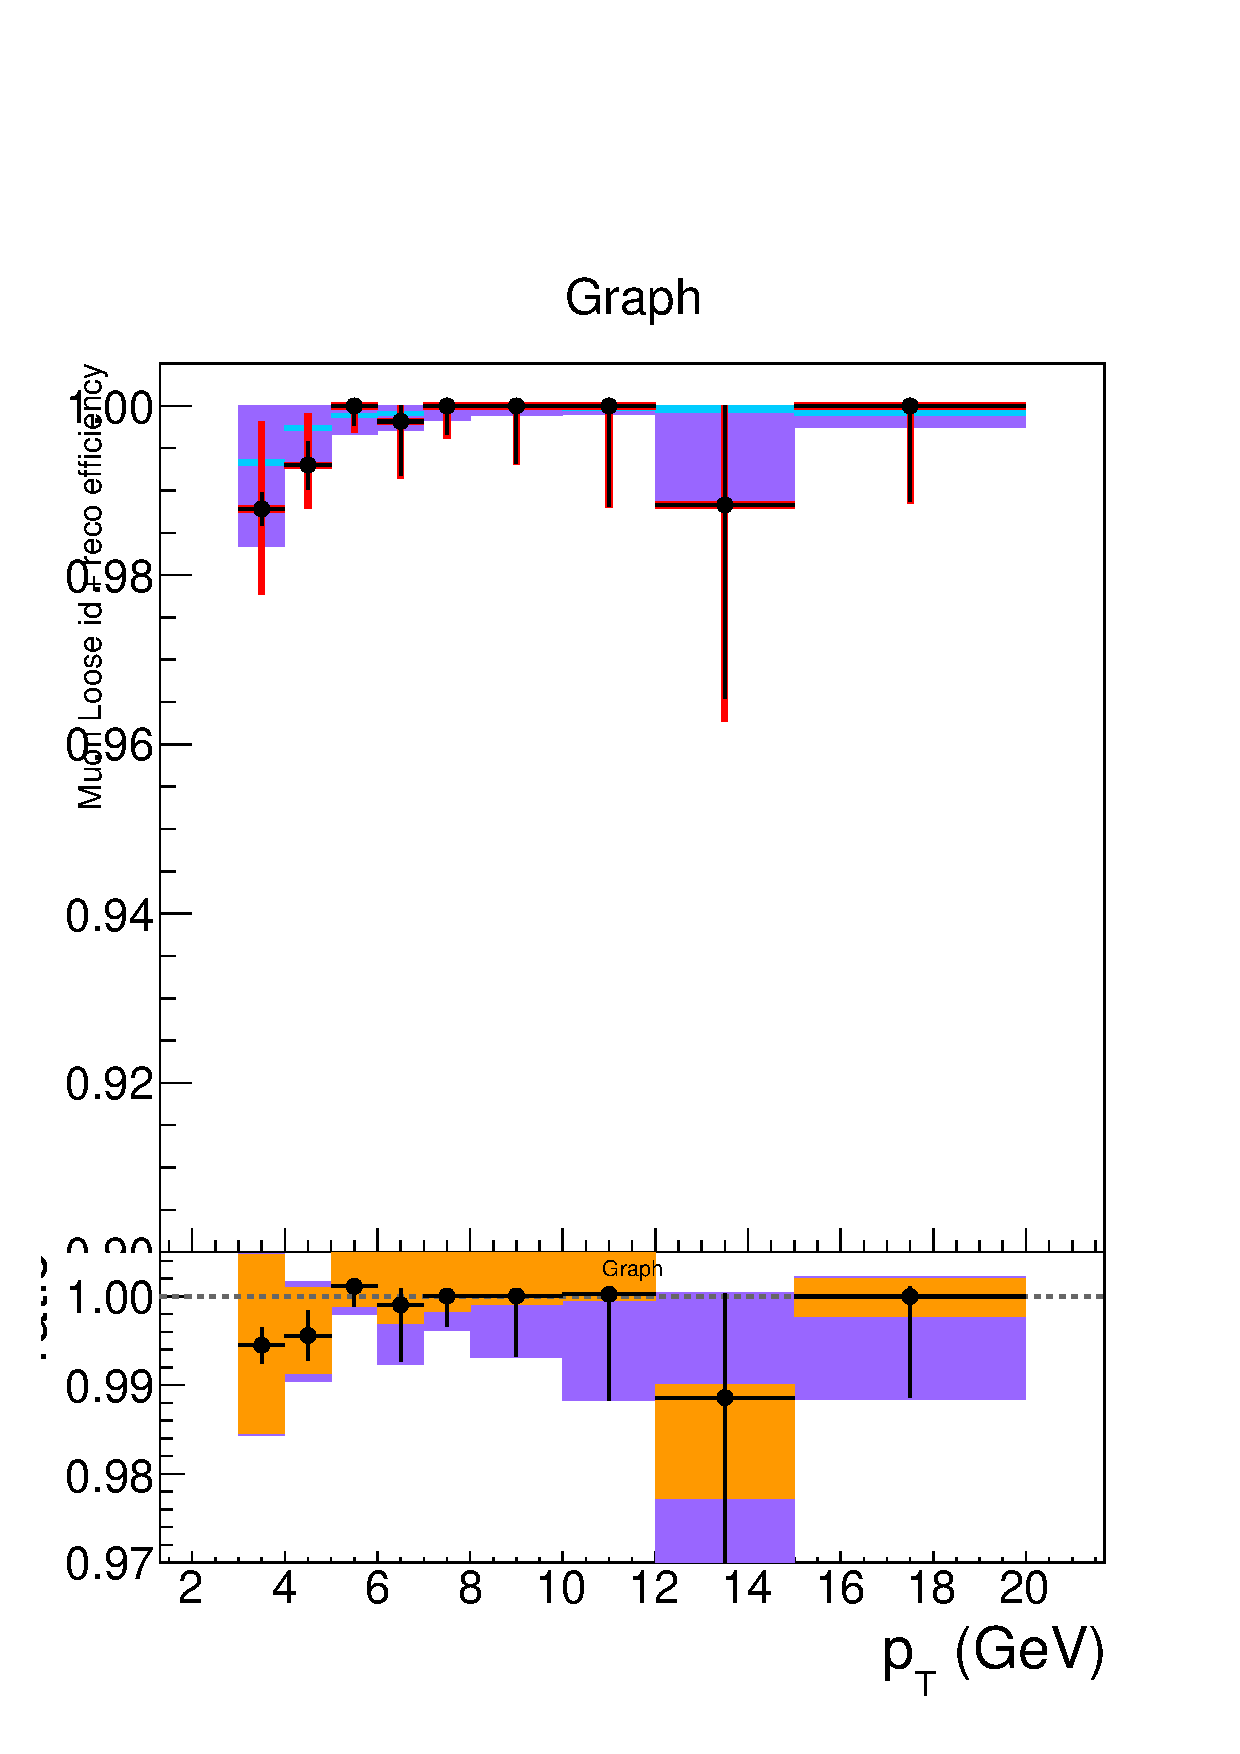
\includegraphics[width=0.32\textwidth]{Figures/Muons/mu_Loose_endcap.pdf}}
%    \subfigure[]{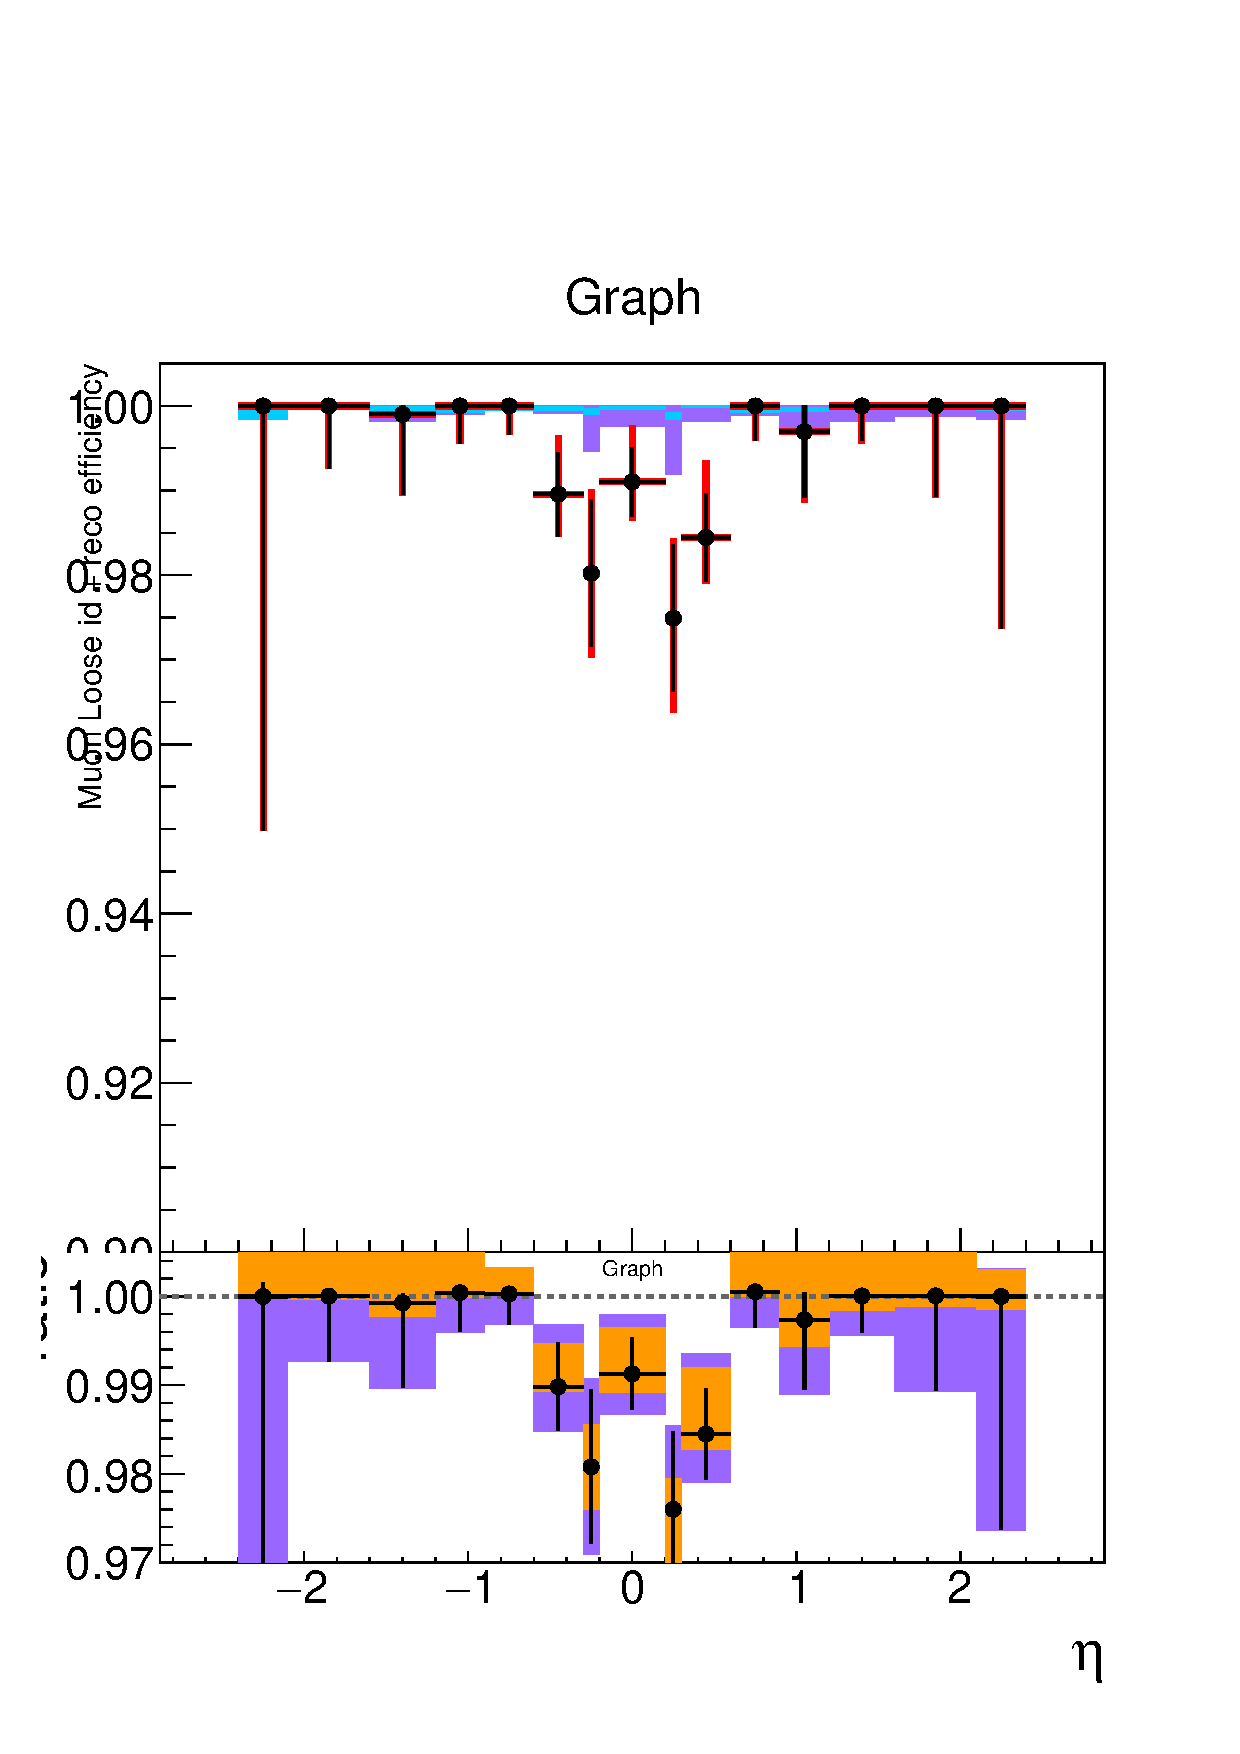
\includegraphics[width=0.32\textwidth]{Figures/Muons/mu_Loose_pt7.pdf}}
%    \caption{Muon reconstruction and identification efficiency at low \pt, measured with the tag\&probe method on \JPsi events, as function of \pt in the barrel (left) and endcaps (center), and as function of $\eta$ for $\pt > 7\GeV$ (right). In the upper panel, the larger error bars include also the systematical uncertainties, while the smaller ones are purely statistical. In the lower panel showing the ratio of the two efficiencies, the black error bars are for the statistical uncertainty, the orange rectangles for the systematical uncertainty and the violet rectangles include both uncertainties.}
%    \label{fig:MuonIDEff_1}
%\end{center}
%\end{figure}

\paragraph*{Impact parameter requirements}
The measurement is performed using $\Z$ events. Events are selected with \verb=HLT_IsoMu20_v*= or \verb=HLT_IsoMu22_v*= triggers.
For this measurement, the probe is a muon passing the POG Loose identification criteria,
and it is considered a passing probe if satisfies the SIP3D, dxy, dz cuts of this analysis.
%
The results are shown in Fig.~\ref{fig:MuonIDEff_2}.
%Very good agreement between data and simulation is observed in the barrel (Fig.~\ref{fig:MuonIDEff_2}, left)
%while some inefficiency is visible in the endcaps, especially at large values of $|\eta|$.
%The data to simulation scale factor is found to be flat as function of \pt, so, similarly to what done
%for the identification part, we apply a correction only as function of $\eta$.


\begin{figure}[tbh]
\centering
\begin{subfigure}{0.25\textwidth}
\centering
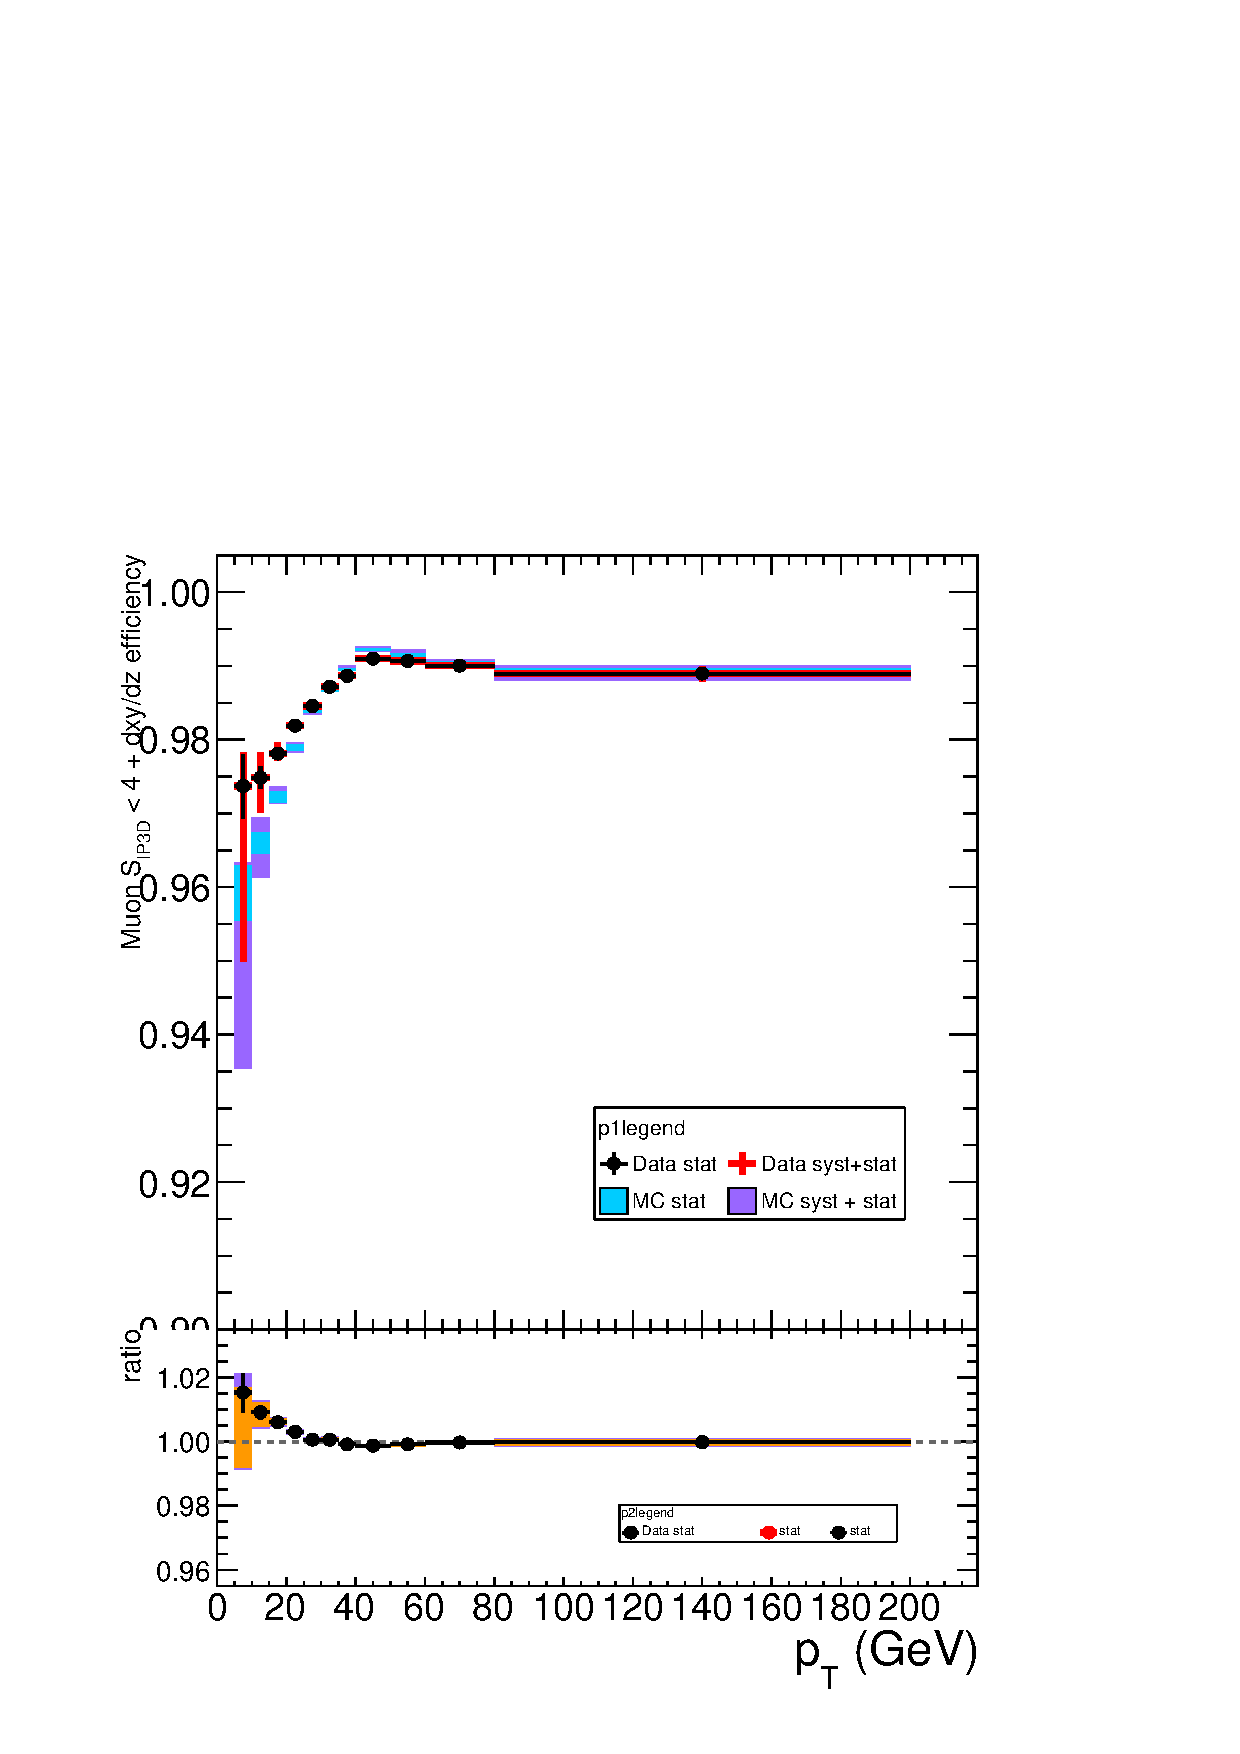
\includegraphics[width=1.5in]{Figures/Muons/mu_SIP4_barrel.pdf}
\caption{}
\end{subfigure}
\begin{subfigure}{0.25\textwidth}
\centering
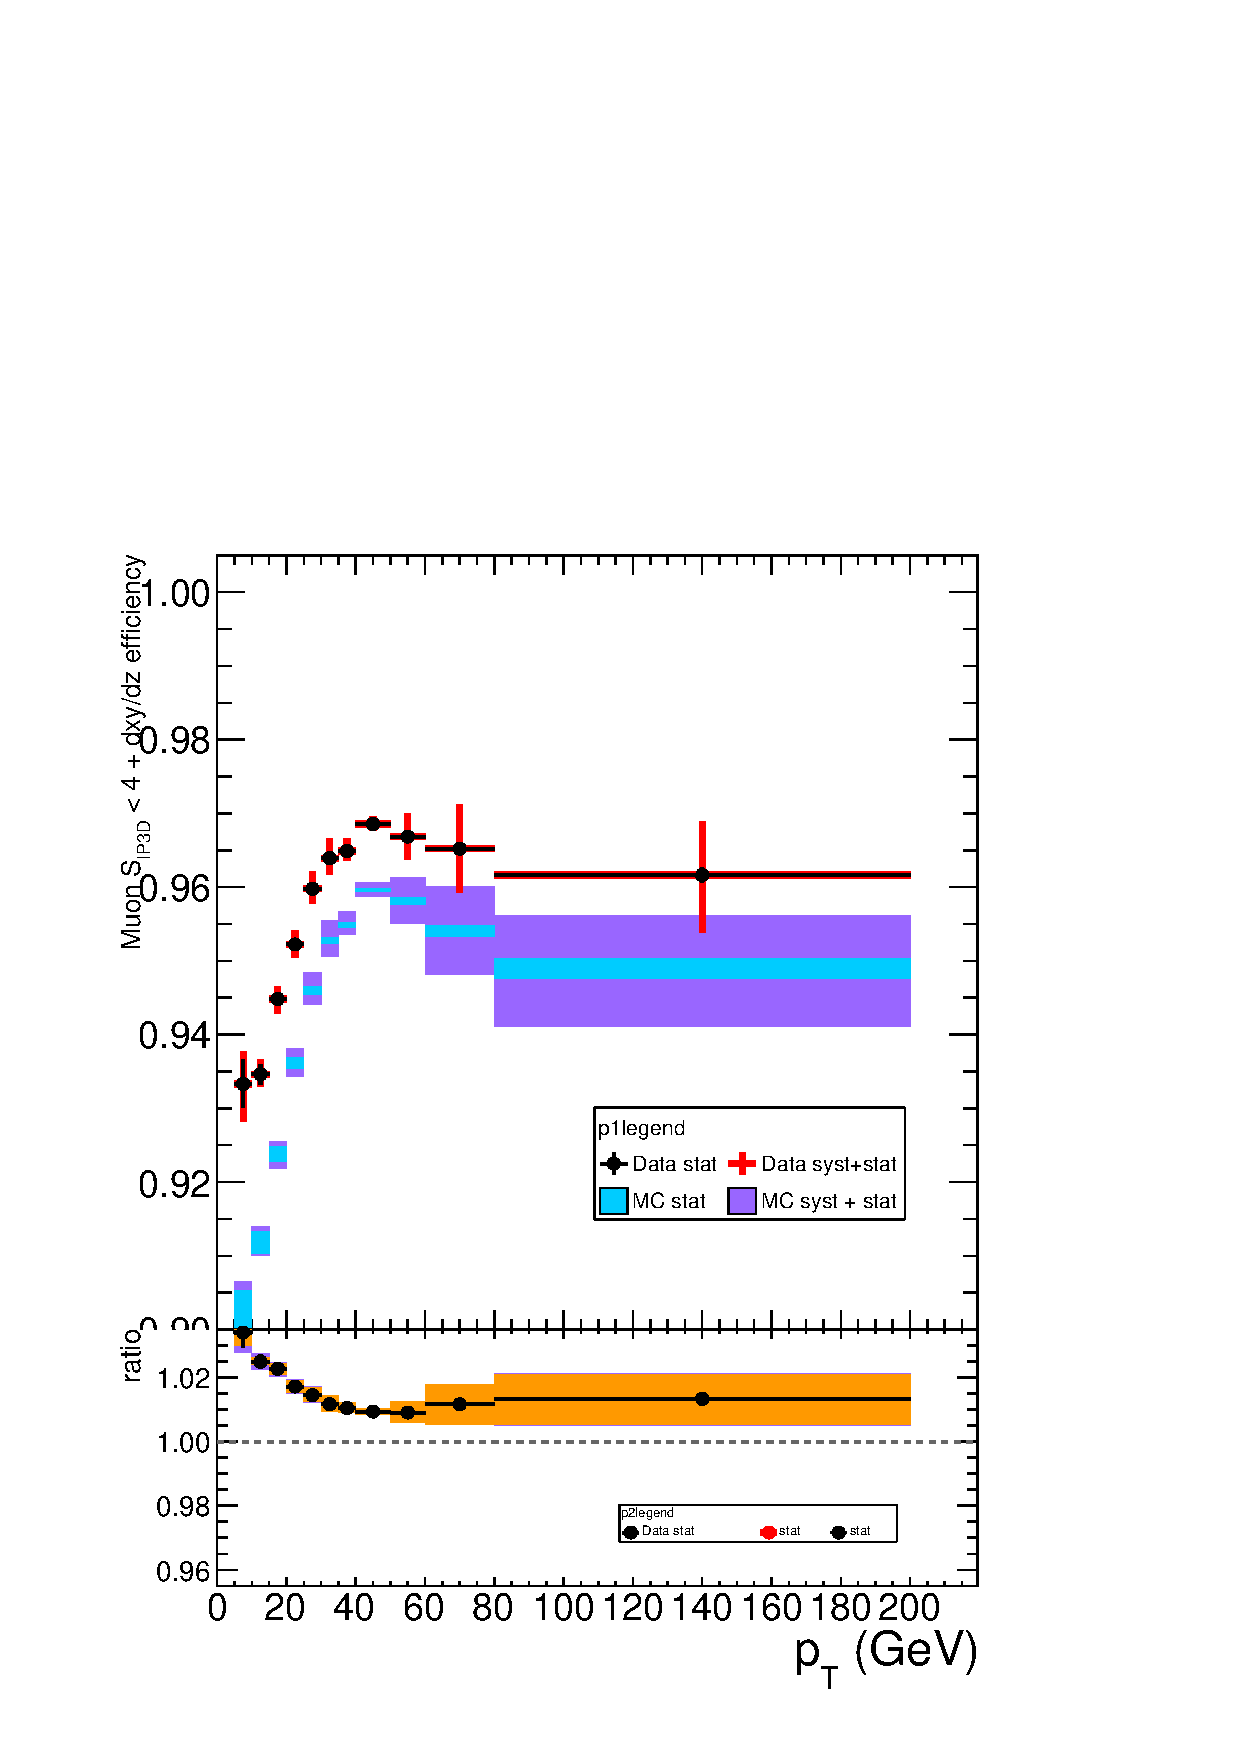
\includegraphics[width=1.5in]{Figures/Muons/mu_SIP4_endcap.pdf}
\caption{}
\end{subfigure}
\begin{subfigure}{0.25\textwidth}
\centering
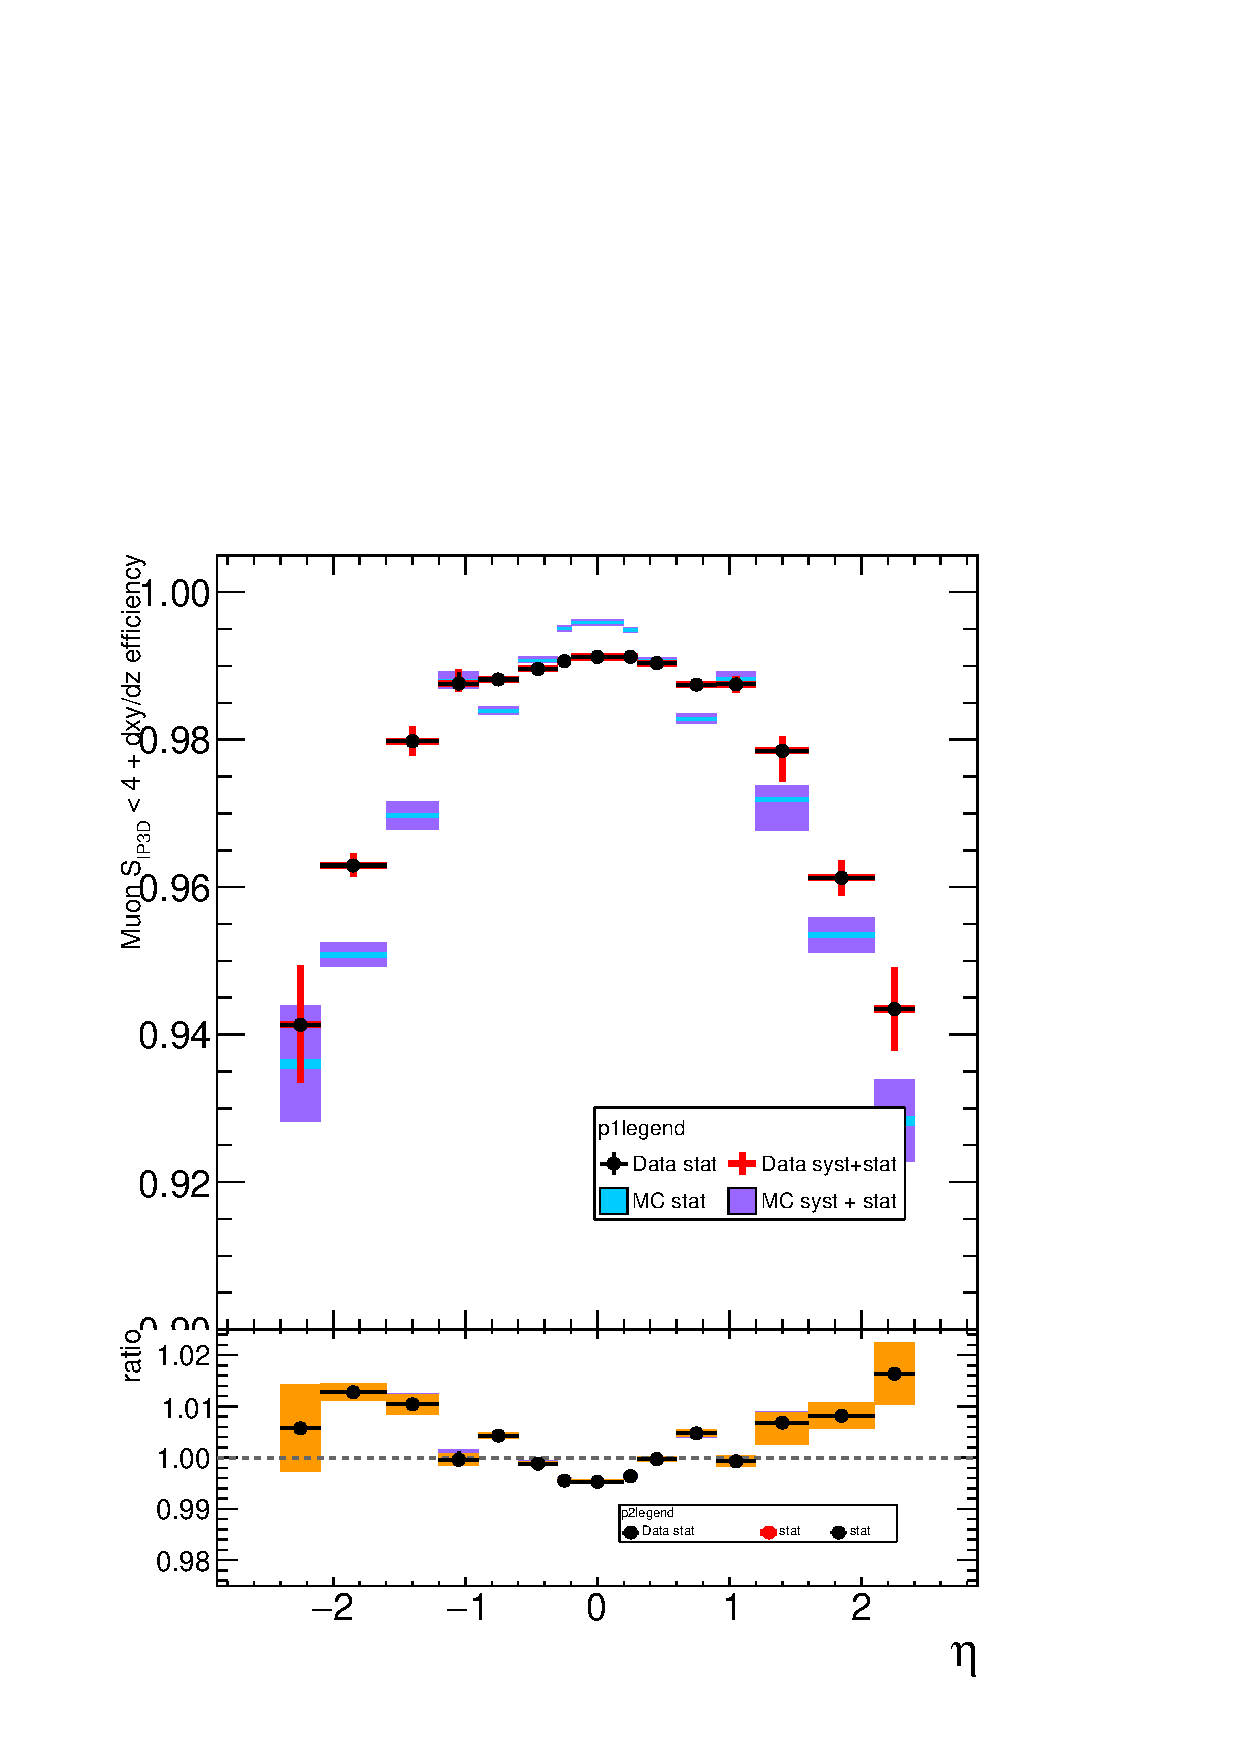
\includegraphics[width=1.5in]{Figures/Muons/mu_SIP4_pt20.pdf}
\caption{}
\end{subfigure}
\caption{Efficiency of the muon impact parameter requirements, measured with the tag\&probe method on \Z events, as function of \pt in the barrel (left) and endcaps (center), and as function of $\eta$ for $\pt > 20\GeV$ (right). In the upper panel, the larger error bars include also the systematical uncertainties, while the smaller ones are purely statistical. In the lower panel showing the ratio of the two efficiencies, the black error bars are for the statistical uncertainty, the orange rectangles for the systematical uncertainty and the violet rectangles include both uncertainties.}
\label{fig:MuonIDEff_2}
\end{figure}

%\begin{figure}[htbp]
%  \begin{center}
%    \subfigure[]{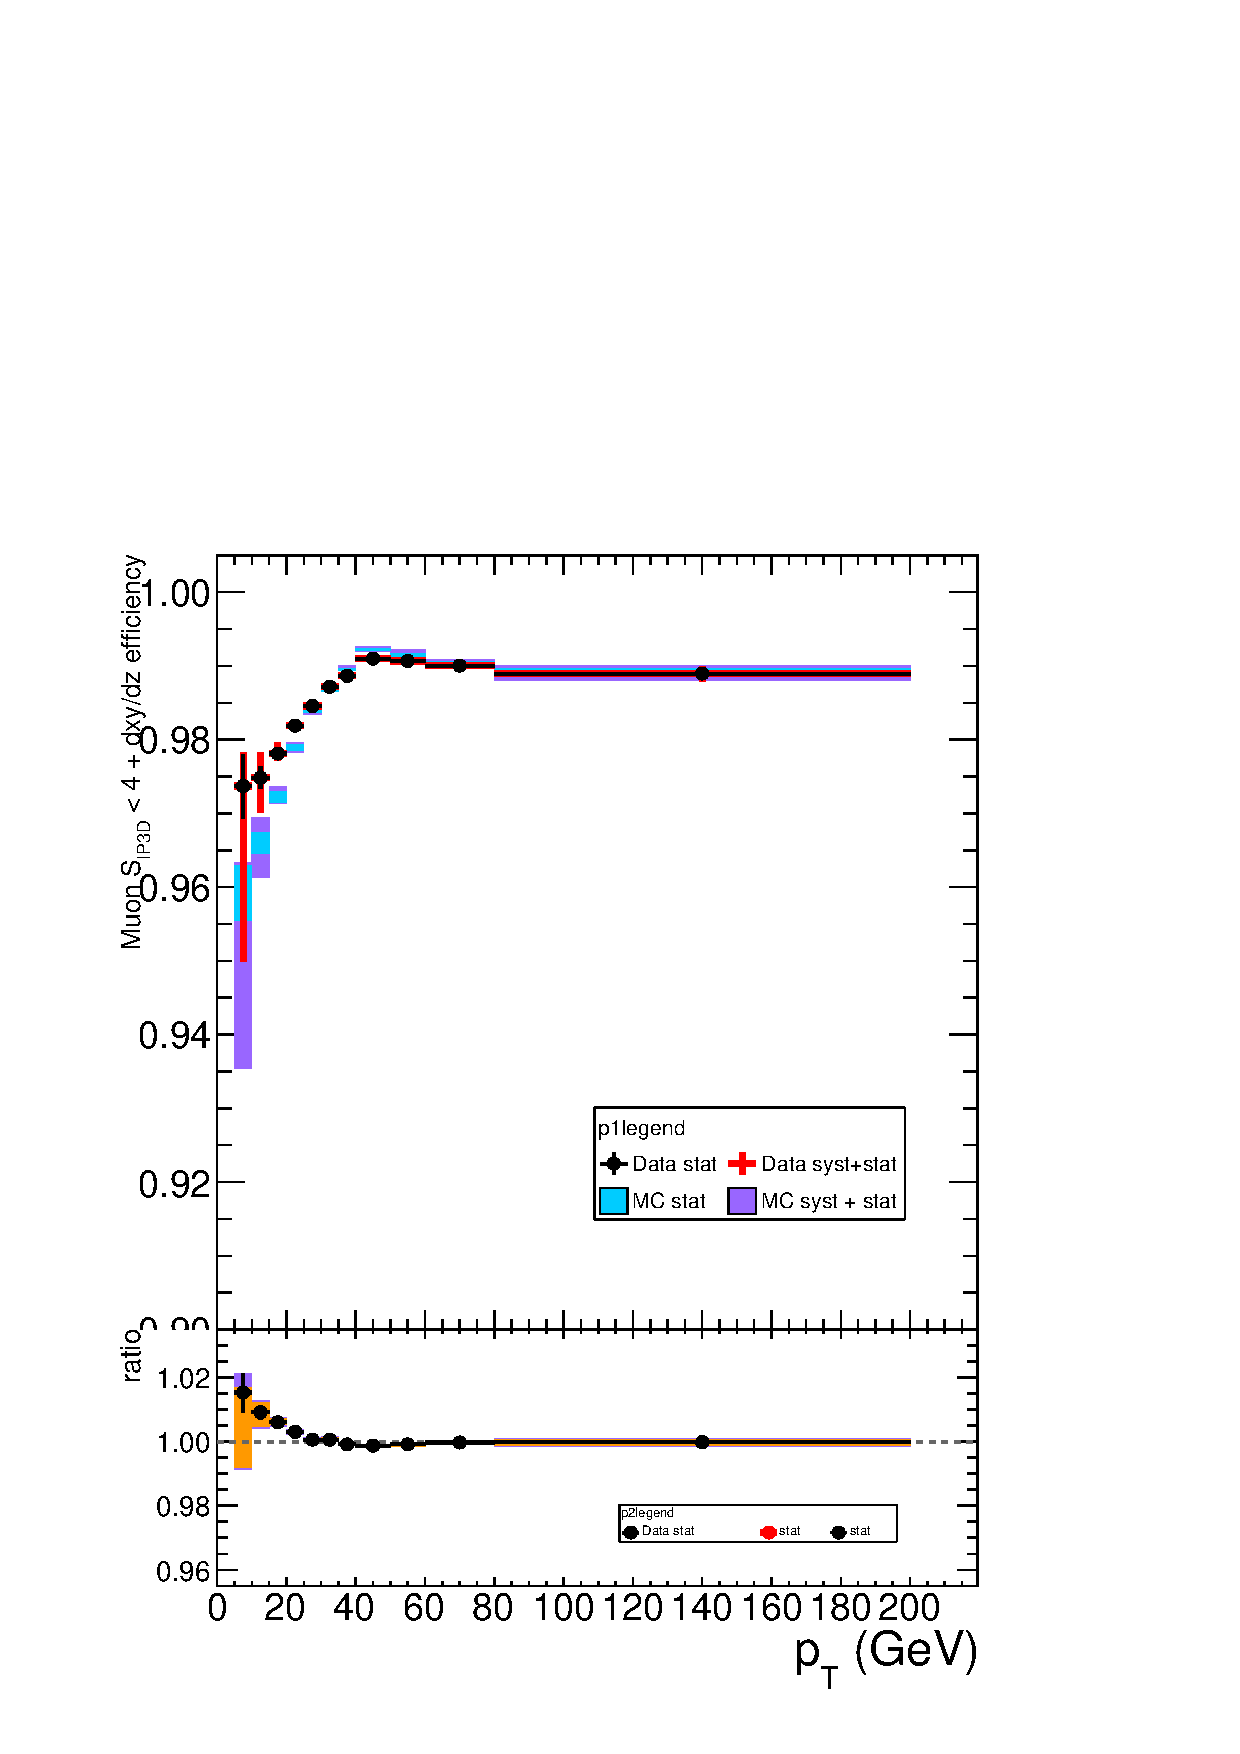
\includegraphics[width=0.32\textwidth]{Figures/Muons/mu_SIP4_barrel.pdf}}
%    \subfigure[]{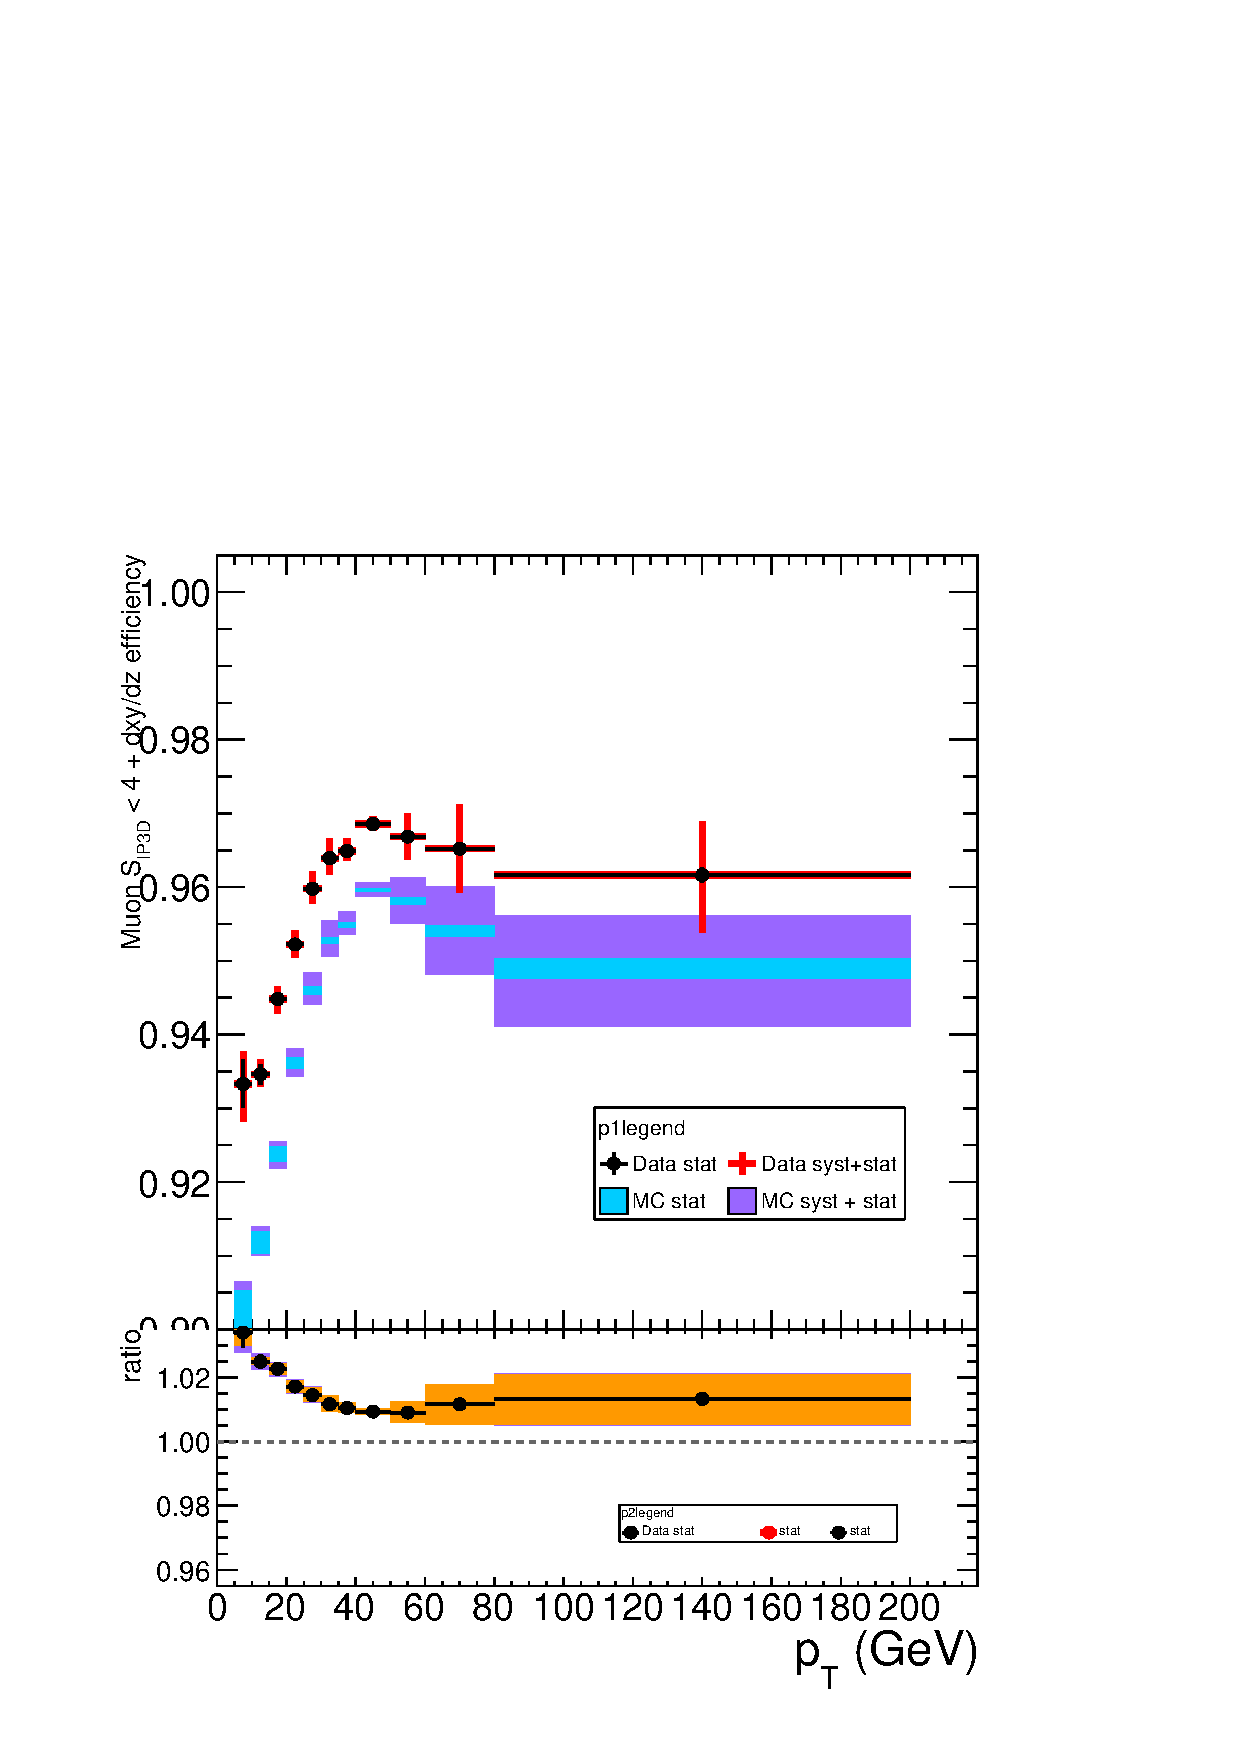
\includegraphics[width=0.32\textwidth]{Figures/Muons/mu_SIP4_endcap.pdf}}
%    \subfigure[]{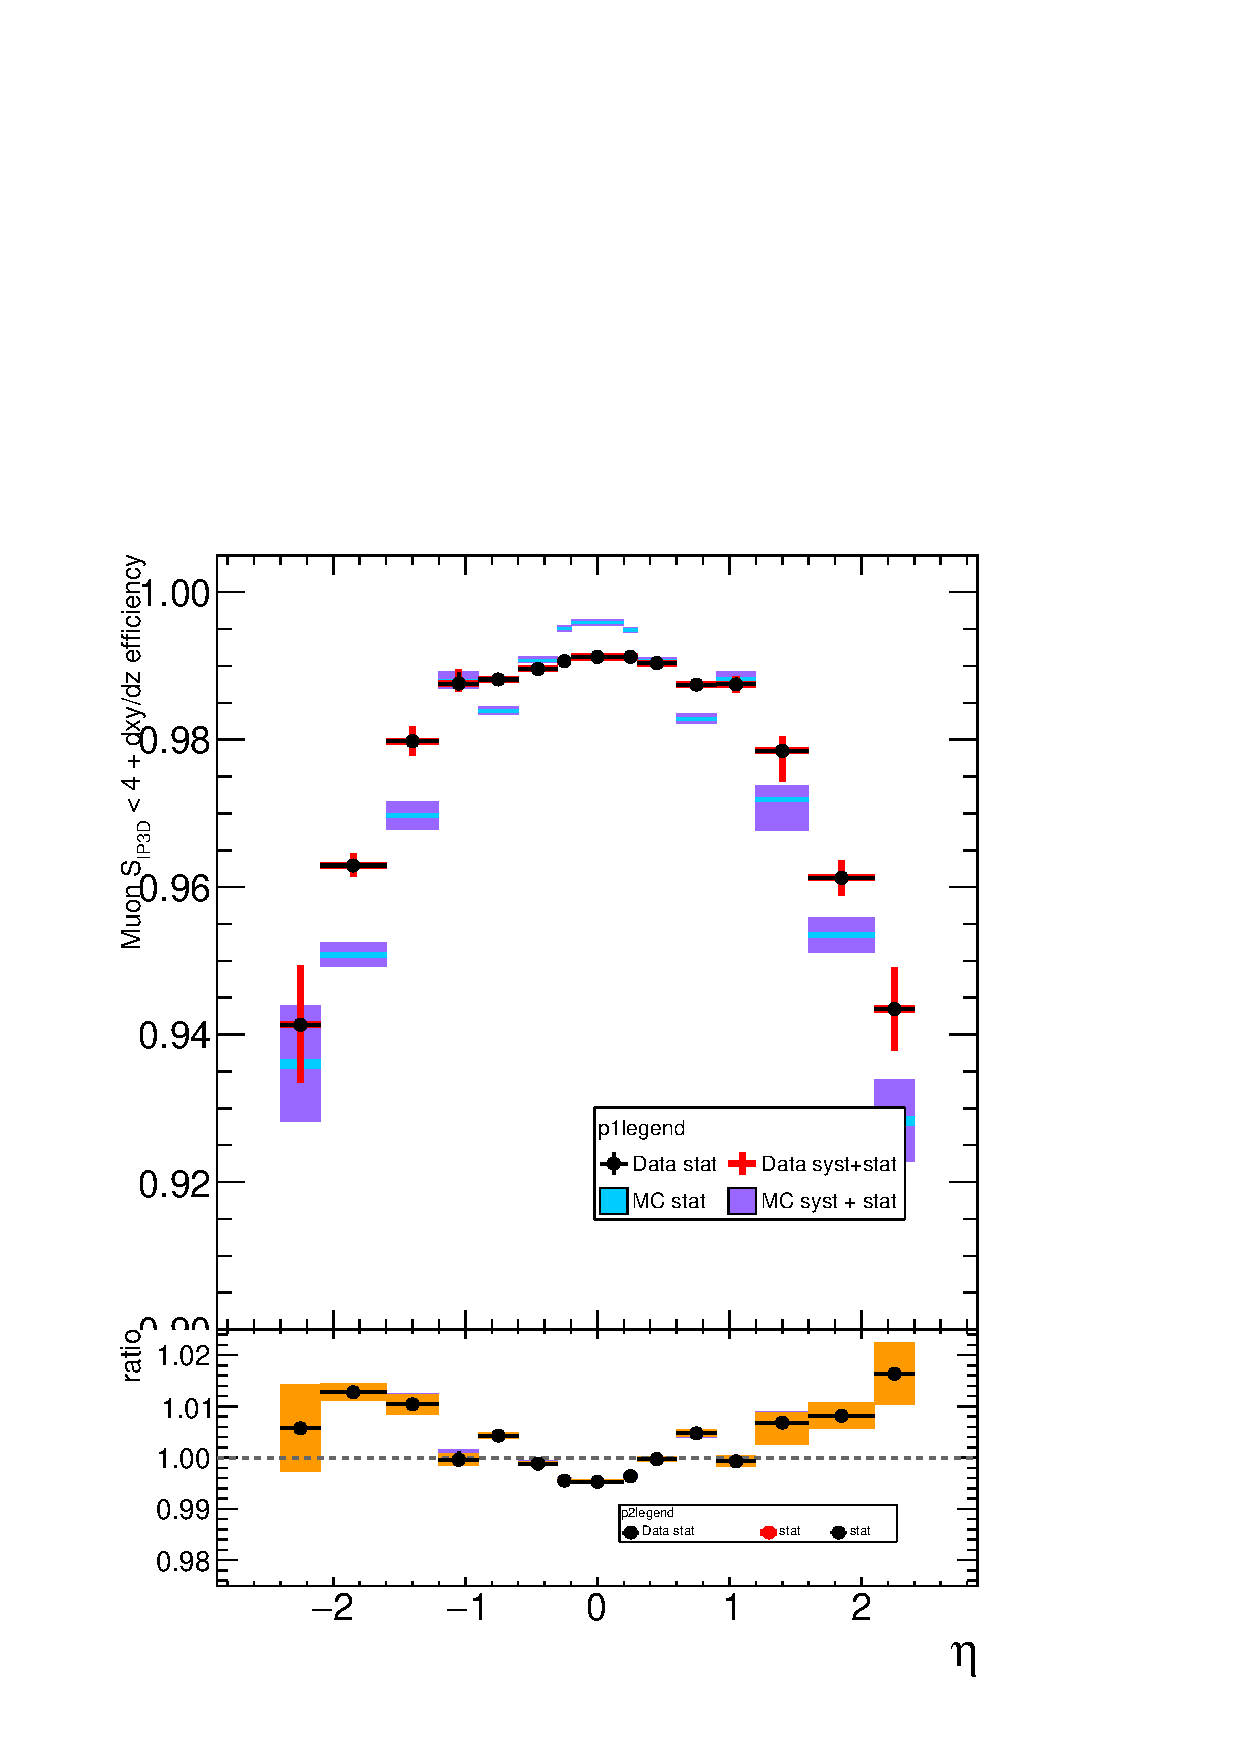
\includegraphics[width=0.32\textwidth]{Figures/Muons/mu_SIP4_pt20.pdf}}
%    \caption{Efficiency of the muon impact parameter requirements, measured with the tag\&probe method on \Z events, as function of \pt in the barrel (left) and endcaps (center), and as function of $\eta$ for $\pt > 20\GeV$ (right). In the upper panel, the larger error bars include also the systematical uncertainties, while the smaller ones are purely statistical. In the lower panel showing the ratio of the two efficiencies, the black error bars are for the statistical uncertainty, the orange rectangles for the systematical uncertainty and the violet rectangles include both uncertainties.}
%    \label{fig:MuonIDEff_2}
%\end{center}
%\end{figure}

\paragraph*{Isolation requirements}
The isolation efficiency is measured using events from the $\Z$ decay for any \pt, selected with either of \verb=HLT_IsoMu20_v*= or \verb=HLT_IsoMu22_v*= triggers. The isolation of the muons are calculated after recovery of the FSR photons and subtracting their contribution to the isolation cone of the muons. More detailed description of the method can be found in Ref.~\cite{AN-16-217}.

The results are shown in Fig.~\ref{fig:MuonIDEff_3}.

\begin{figure}[tbh]
\centering
\begin{subfigure}{0.45\textwidth}
\centering
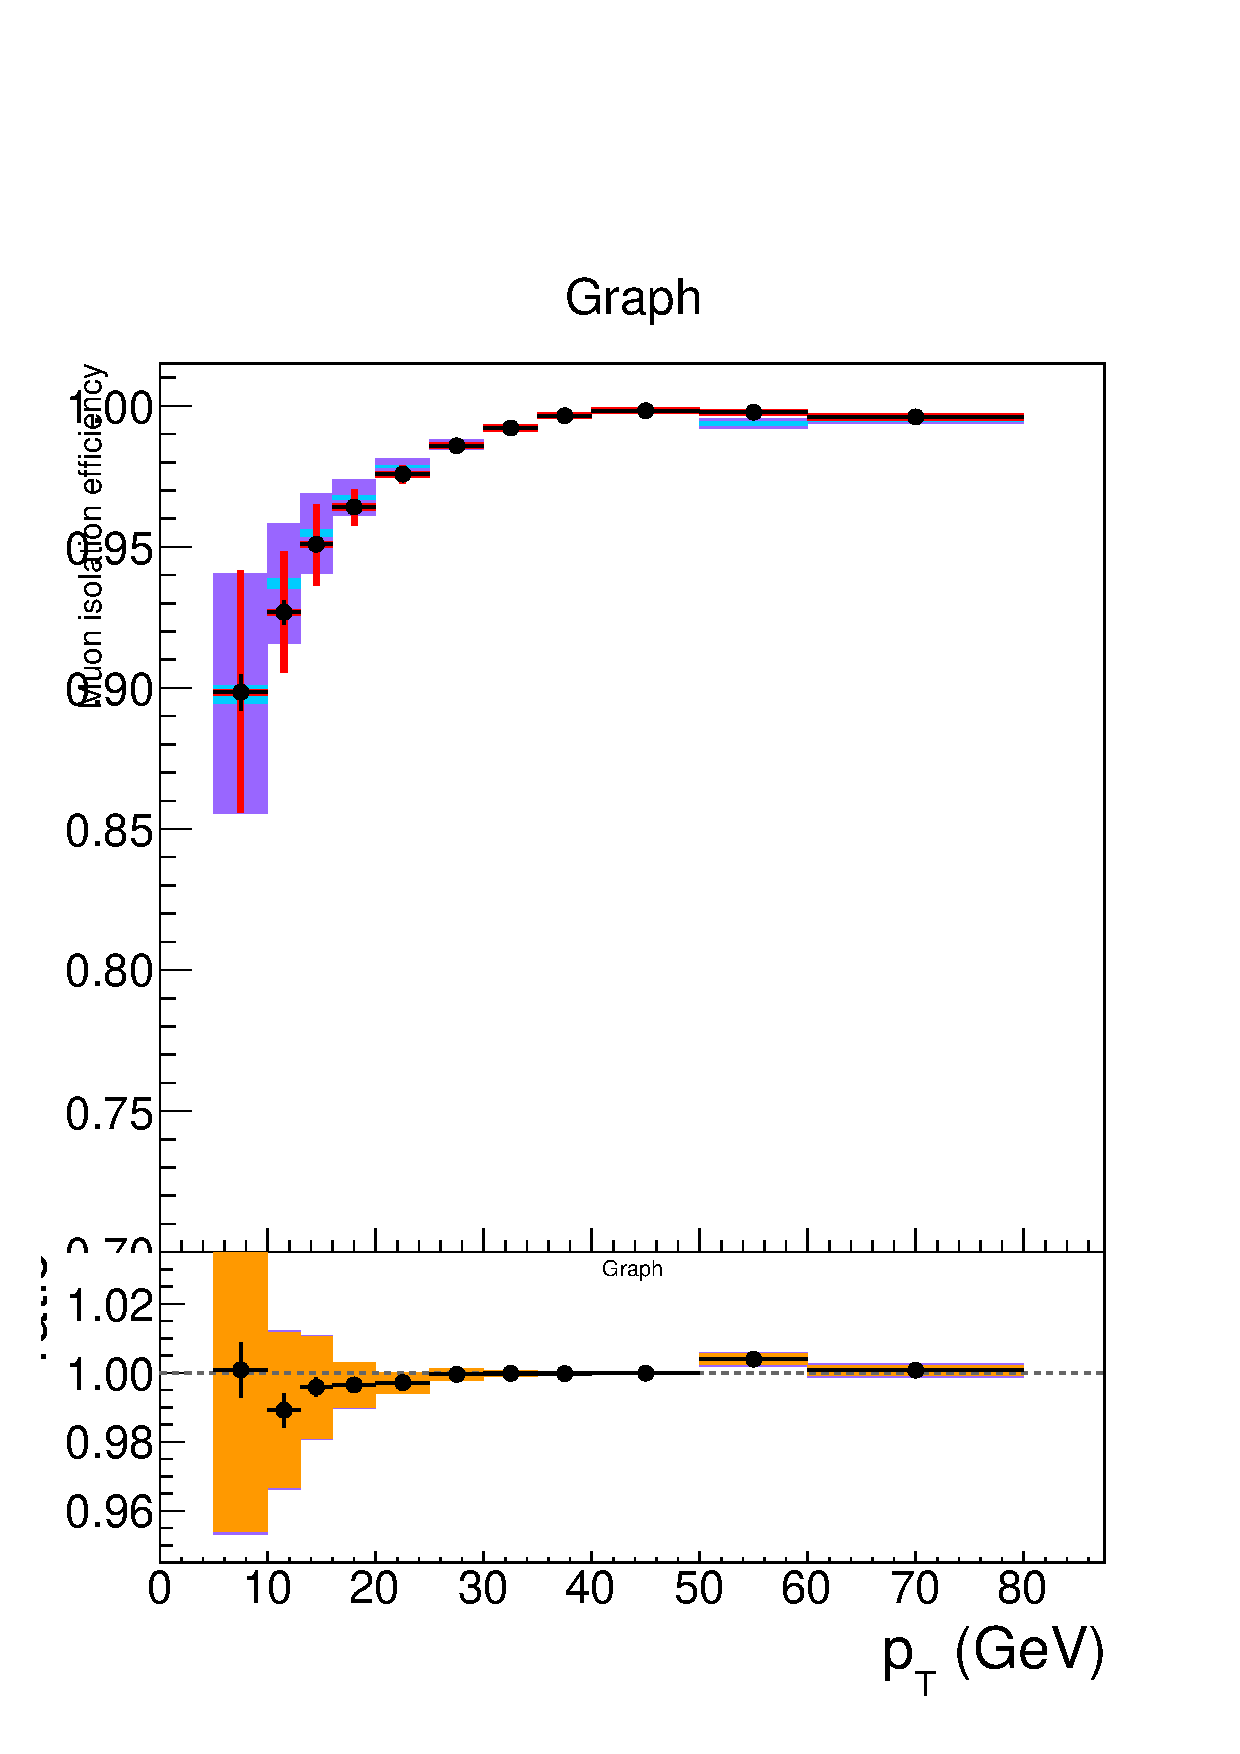
\includegraphics[width=2.5in]{Figures/Muons/mu_iso_barrel.pdf}
\caption{}
\end{subfigure}
\begin{subfigure}{0.45\textwidth}
\centering
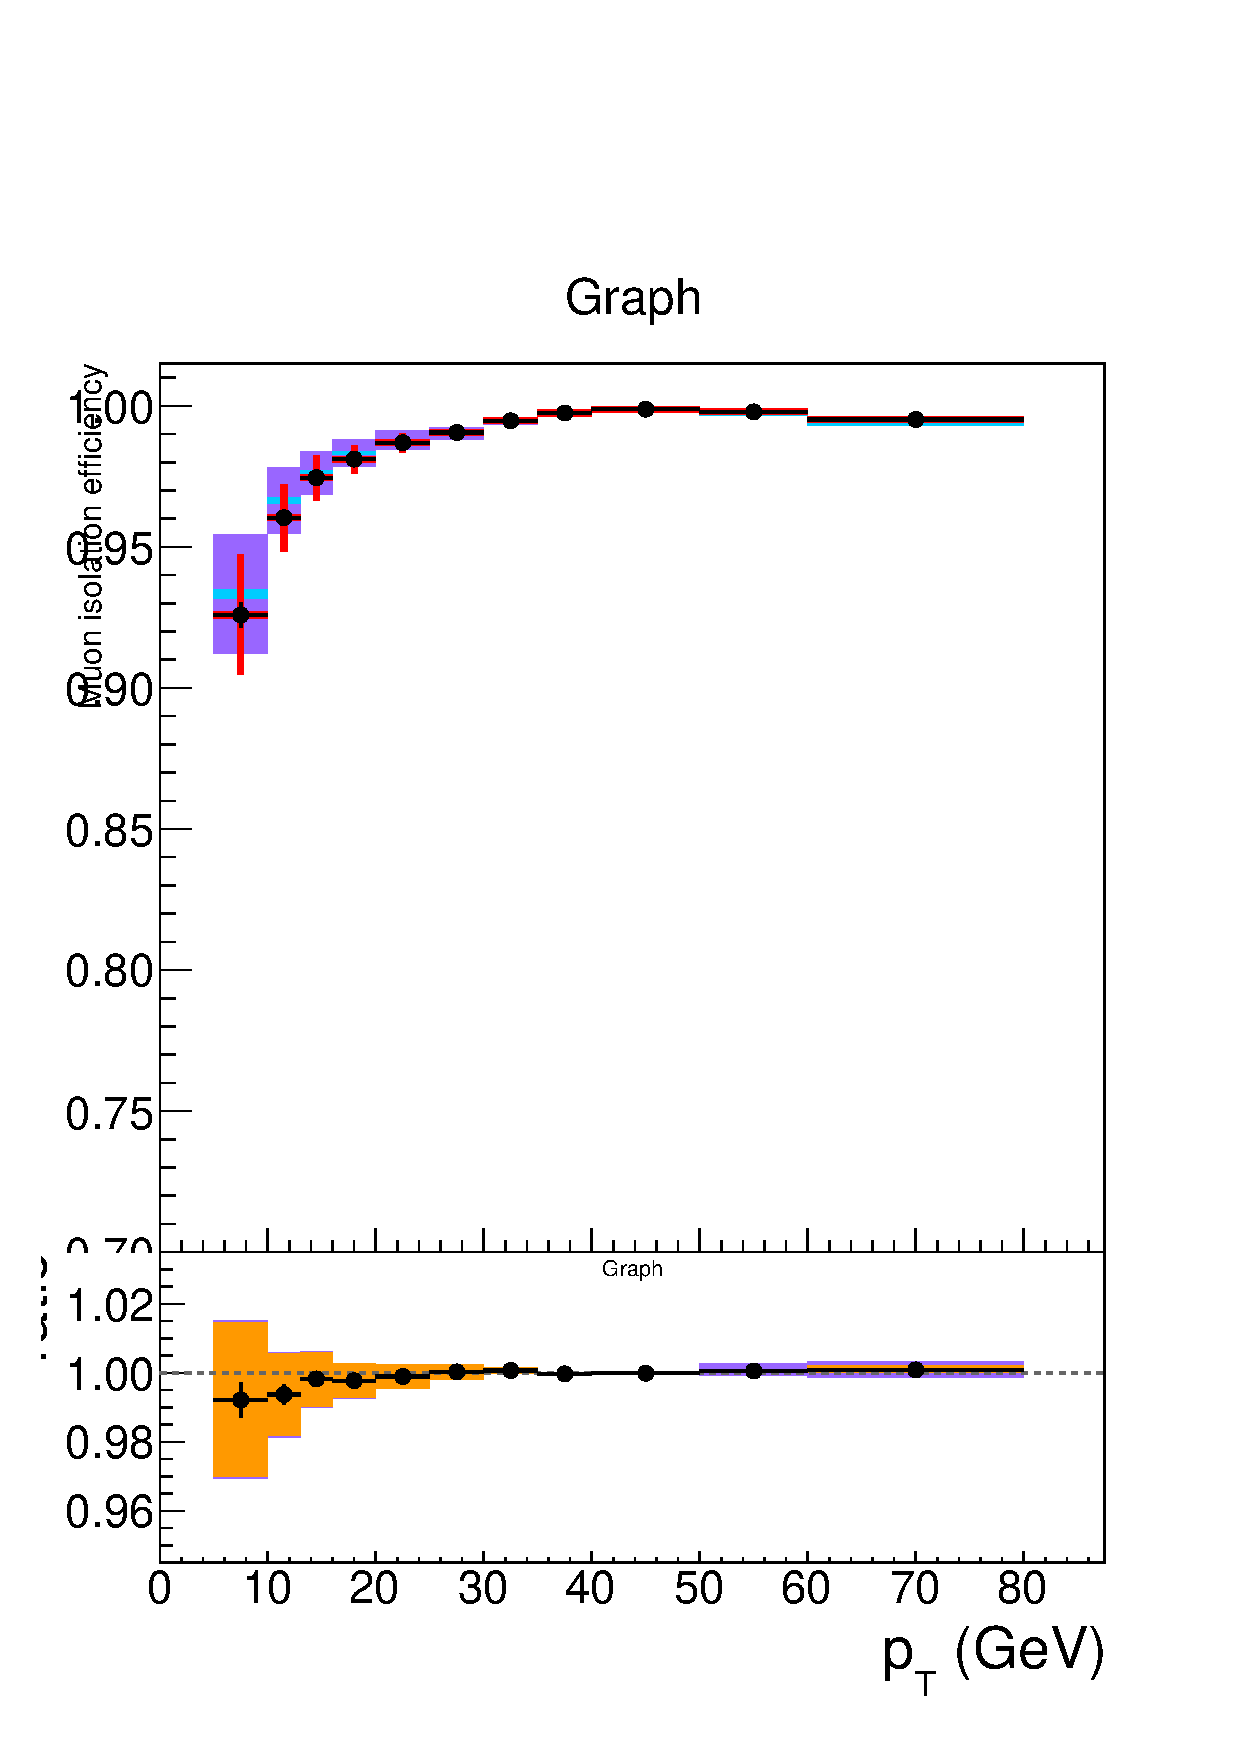
\includegraphics[width=2.5in]{Figures/Muons/mu_iso_endcap.pdf}
\caption{}
\end{subfigure}
    \caption{Efficiency of the muon isolation requirement, measured with the tag\&probe method on \Z events, as function of \pt in the barrel (left) and endcaps (right). In the upper panel, the larger error bars include also the systematical uncertainties, while the smaller ones are purely statistical. In the lower panel showing the ratio of the two efficiencies, the black error bars are for the statistical uncertainty, the orange rectangles for the systematical uncertainty and the violet rectangles include both uncertainties.}
\label{fig:MuonIDEff_3}
\end{figure}

%\begin{figure}[htbp]
%  \begin{center}
%    \subfigure[]{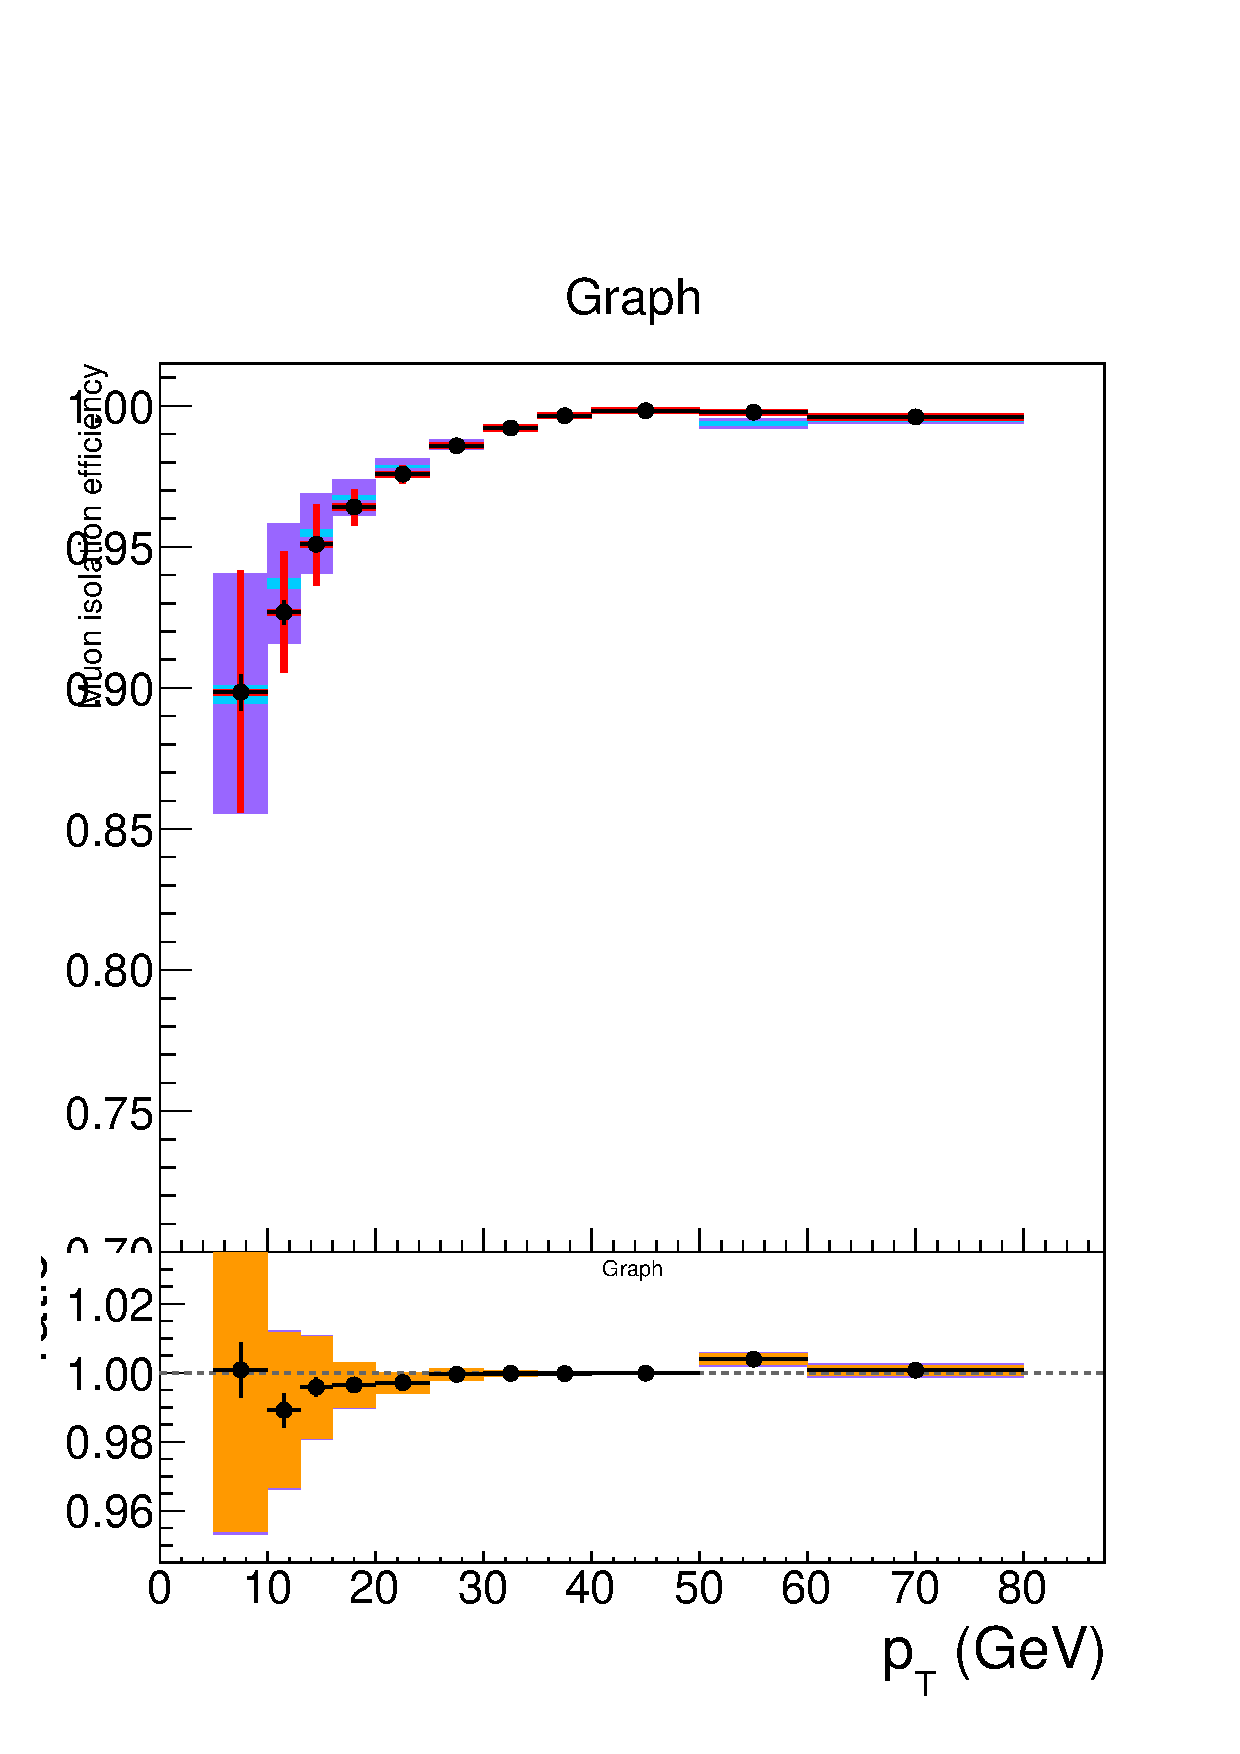
\includegraphics[width=0.32\textwidth]{Figures/Muons/mu_iso_barrel.pdf}}
%    \subfigure[]{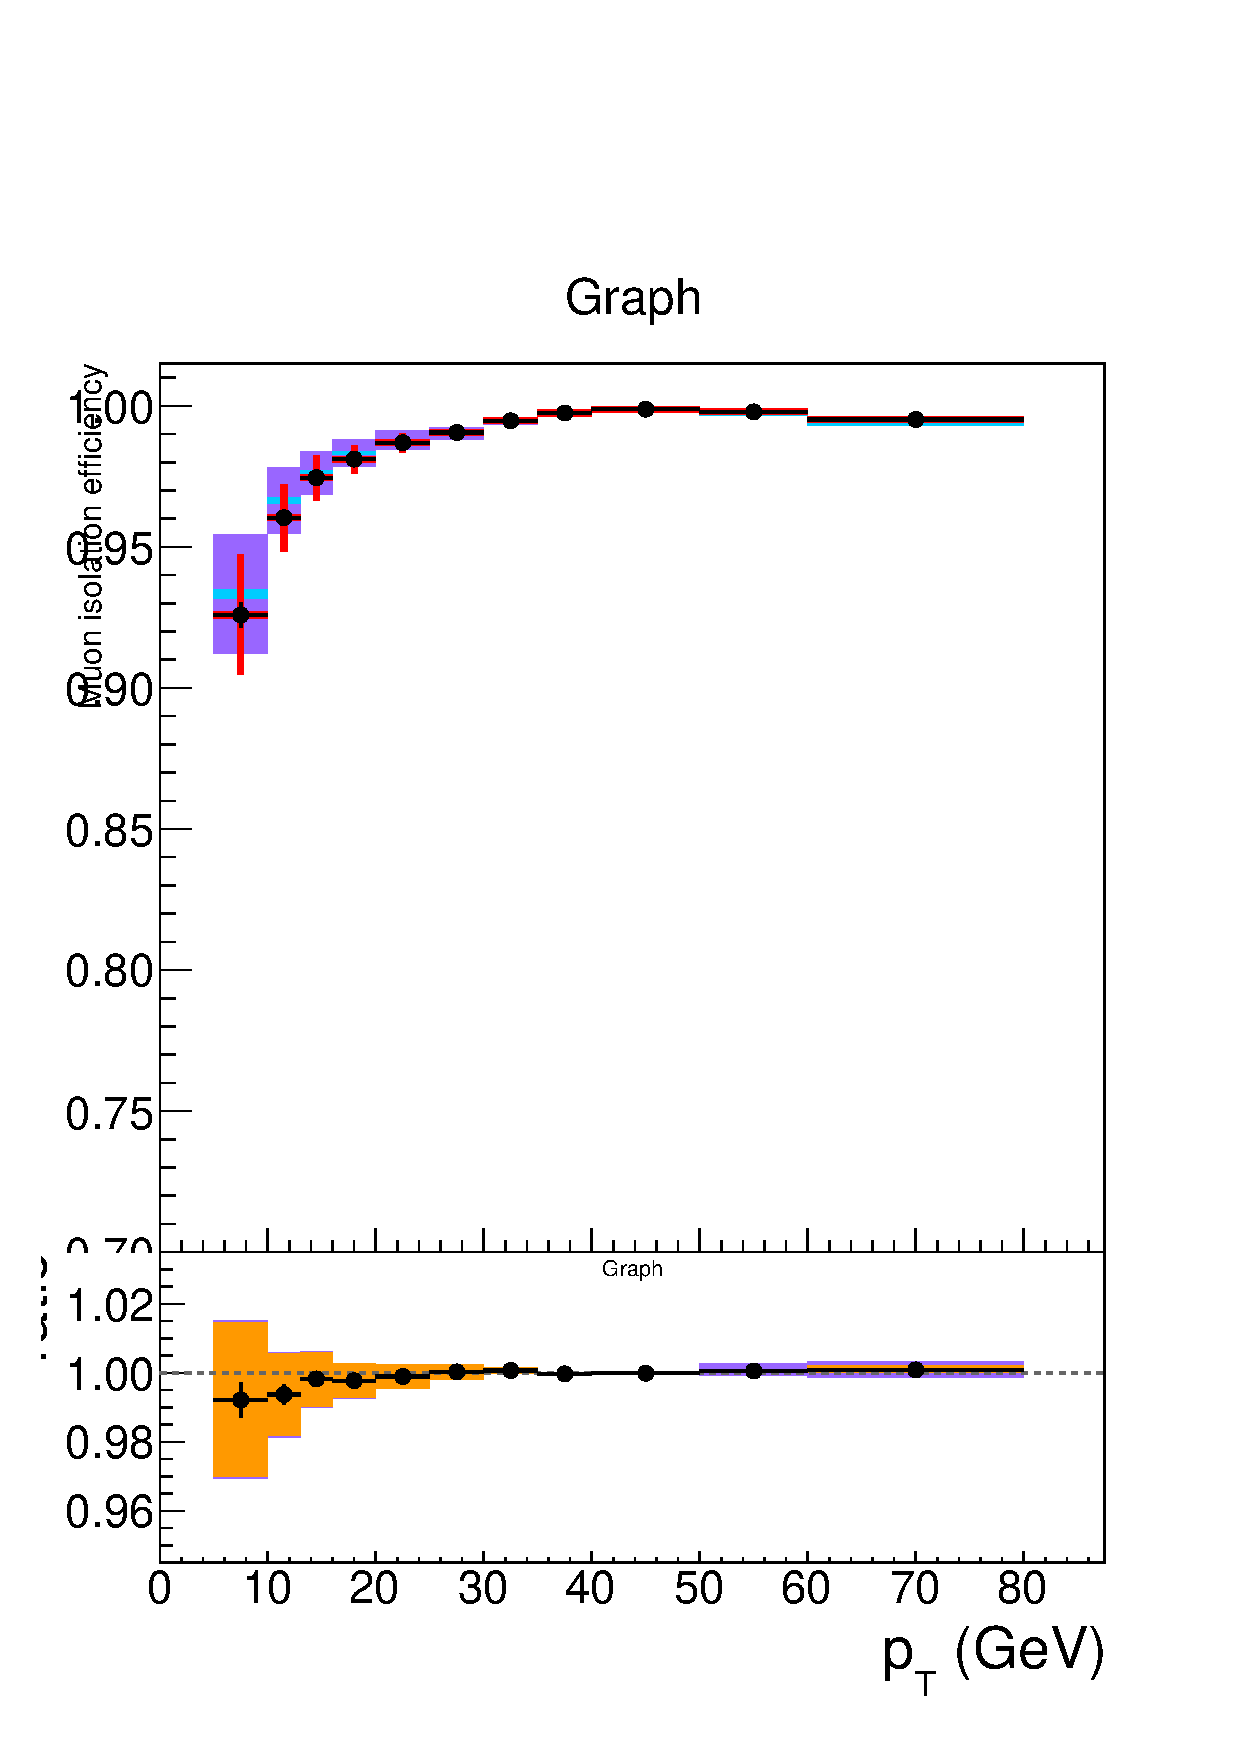
\includegraphics[width=0.32\textwidth]{Figures/Muons/mu_iso_endcap.pdf}}
%    \caption{Efficiency of the muon isolation requirement, measured with the tag\&probe method on \Z events, as function of \pt in the barrel (left) and endcaps (right). In the upper panel, the larger error bars include also the systematical uncertainties, while the smaller ones are purely statistical. In the lower panel showing the ratio of the two efficiencies, the black error bars are for the statistical uncertainty, the orange rectangles for the systematical uncertainty and the violet rectangles include both uncertainties.}
%    \label{fig:MuonIDEff_3}
%\end{center}
%\end{figure}

\paragraph*{Tracking}
The efficiency to reconstruct a muon track in the inner detector is measured using as probes tracks
reconstructed in the muon system alone. The method for measuring the tracking efficiency is the same as 
 in Ref.~\cite{CMS_AN_2015-215}, and the results on 2016 data are briefly discussed here. The efficiency and 
data to mc scale factors are measured from Z events as a function of $\eta$ for $\pt > 10\GeV$ and $\pt < 10\GeV$. The values of data to mc scale factors 
used are from the ReReco version of the full dataset collected in 2016. 

The tracking efficiency in data and simulation as a function of $\eta$ is shown in Fig.~\ref{fig:MuonIDEff_4}.

\begin{figure}[tbh]
\centering
\begin{subfigure}{0.45\textwidth}
\centering
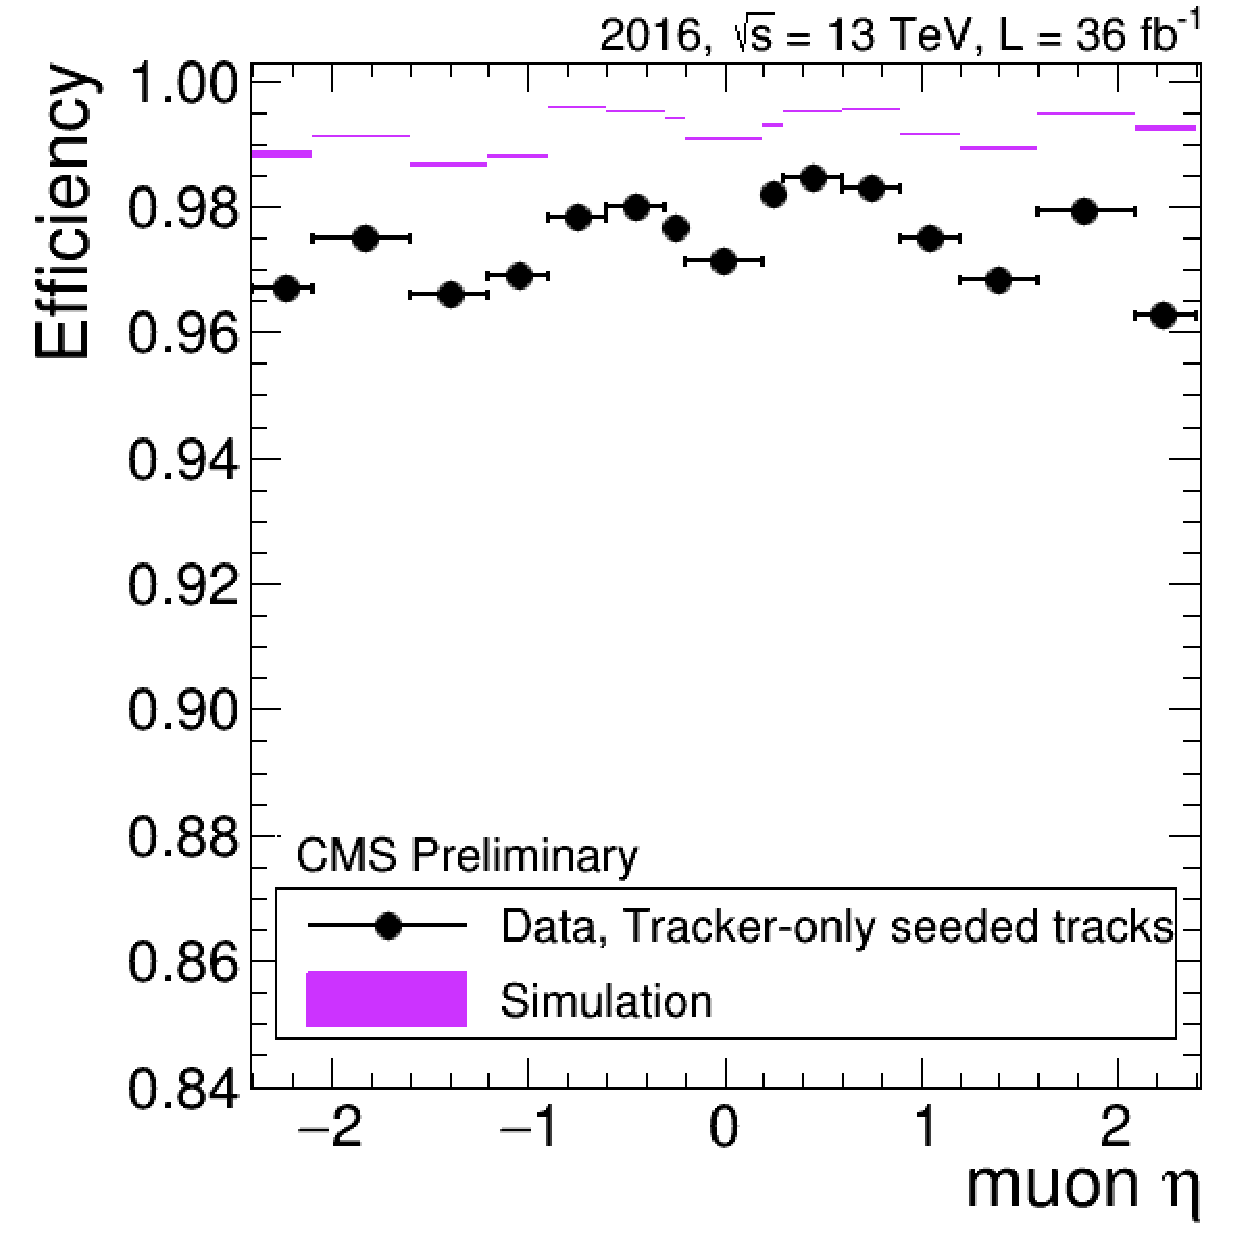
\includegraphics[width=2.5in]{Figures/Muons/trackingEffptl10.pdf}
\caption{}
\end{subfigure}
\begin{subfigure}{0.45\textwidth}
\centering
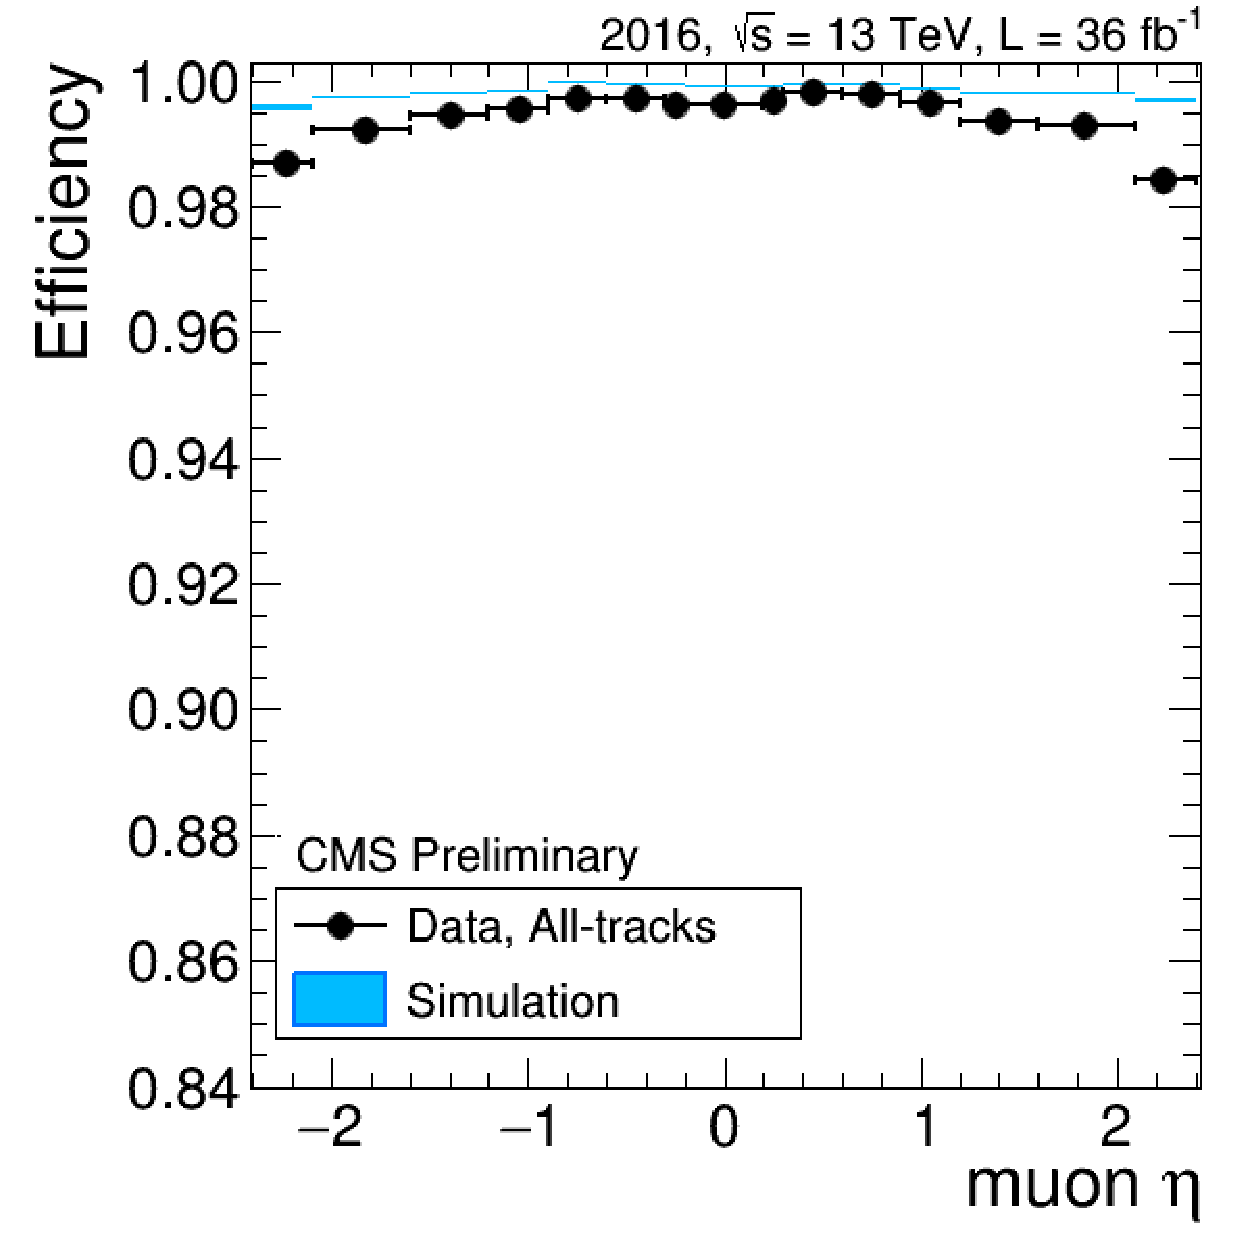
\includegraphics[width=2.5in]{Figures/Muons/trackingEffptg10.pdf}
\caption{}
\end{subfigure}
    \caption{Tracking efficiency in data and simulation as a function of $\eta$ for muon $\pt < 10\GeV$(left) and $\pt > 10\GeV$(right) with ReReco data.}
    \label{fig:MuonIDEff_4}
\end{figure}

%\begin{figure}[htbp]
%  \begin{center}
%    \subfigure[]{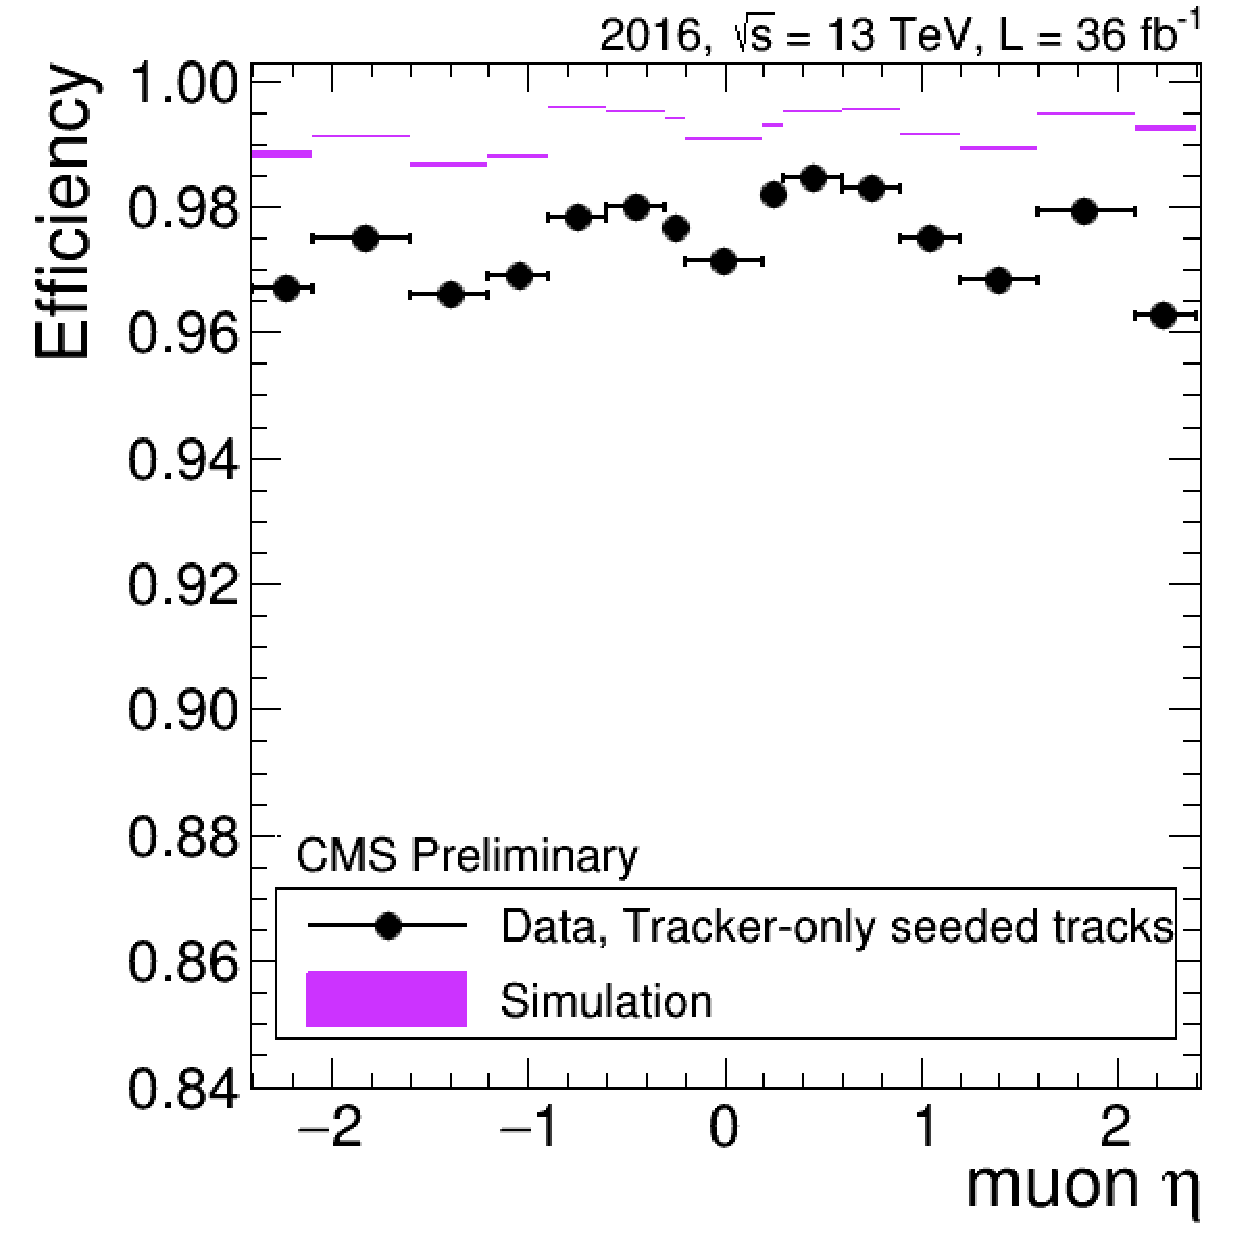
\includegraphics[width=0.42\textwidth]{Figures/Muons/trackingEffptl10.pdf}}
%    \subfigure[]{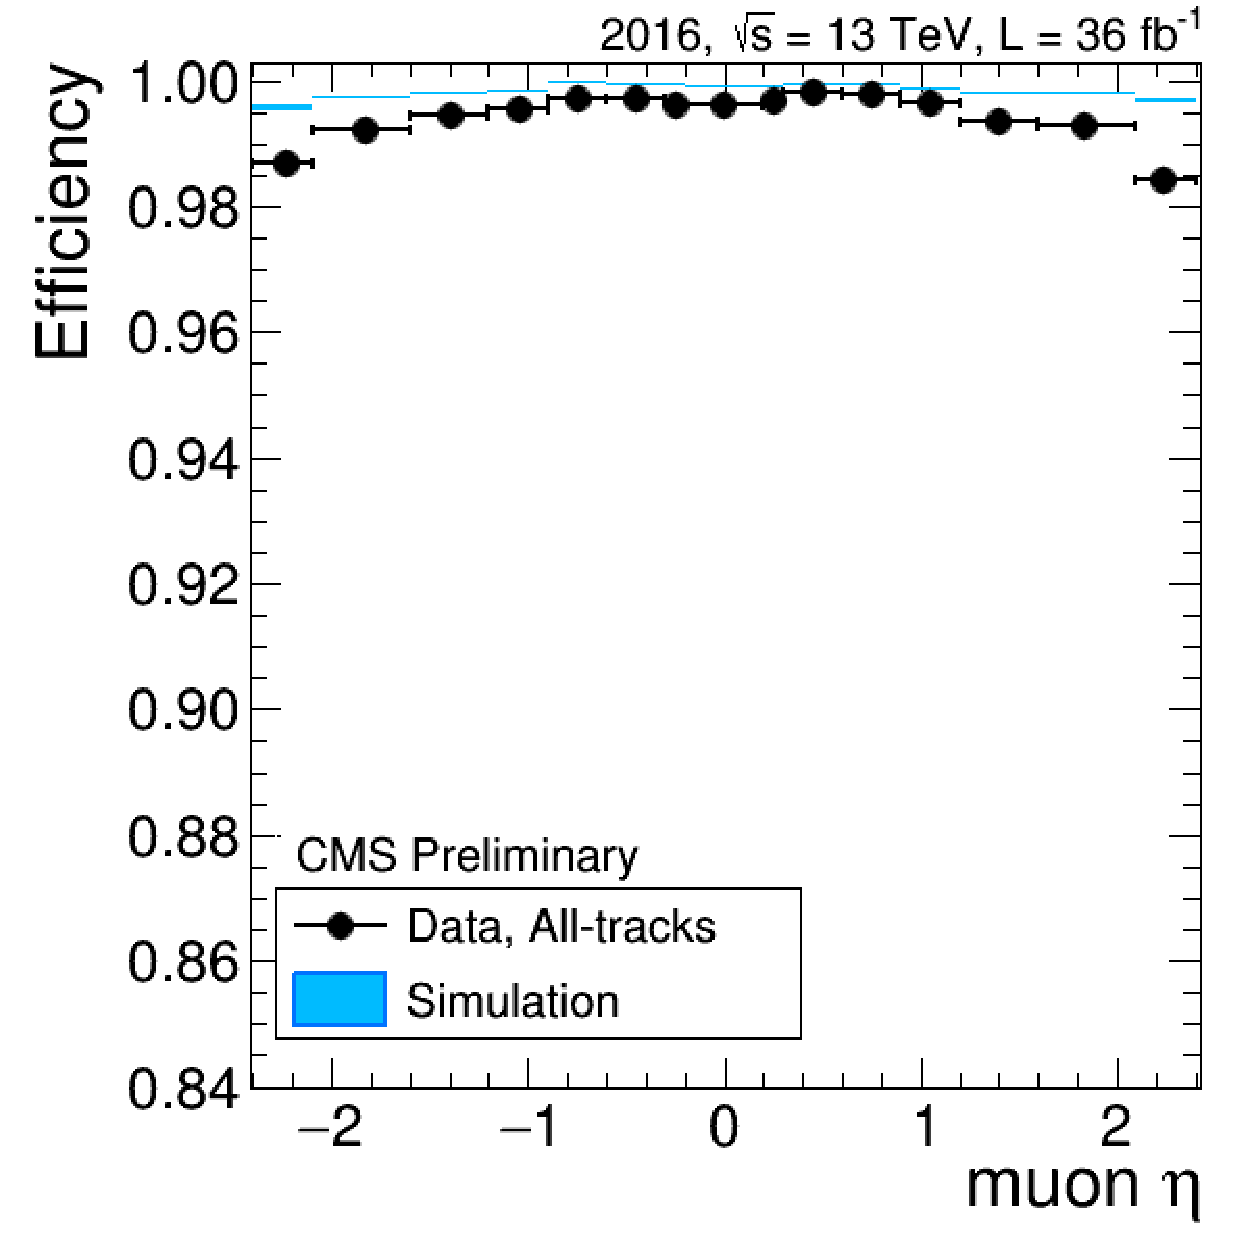
\includegraphics[width=0.42\textwidth]{Figures/Muons/trackingEffptg10.pdf}}
%    \caption{Tracking efficiency in data and simulation as a function of $\eta$ for muon $\pt < 10\GeV$(left) and $\pt > 10\GeV$(right) with ReReco data.}
%    \label{fig:MuonIDEff_4}
%\end{center}
%\end{figure}

\paragraph*{Overall results}
The product of all the data to simulation scale factors for muon tracking, reconstruction, identification, impact parameter and isolation requirements is shown in Fig.~\ref{fig:MuonIDEff_5}. 
%The overall correction is about $-1\%$ or less for most \pt and $\eta$ values, increasing to about $-2\%$ in for muons below $10\GeV$ or with $|\eta|>2$.

\begin{figure}[tbh]
\centering
\begin{subfigure}{0.45\textwidth}
\centering
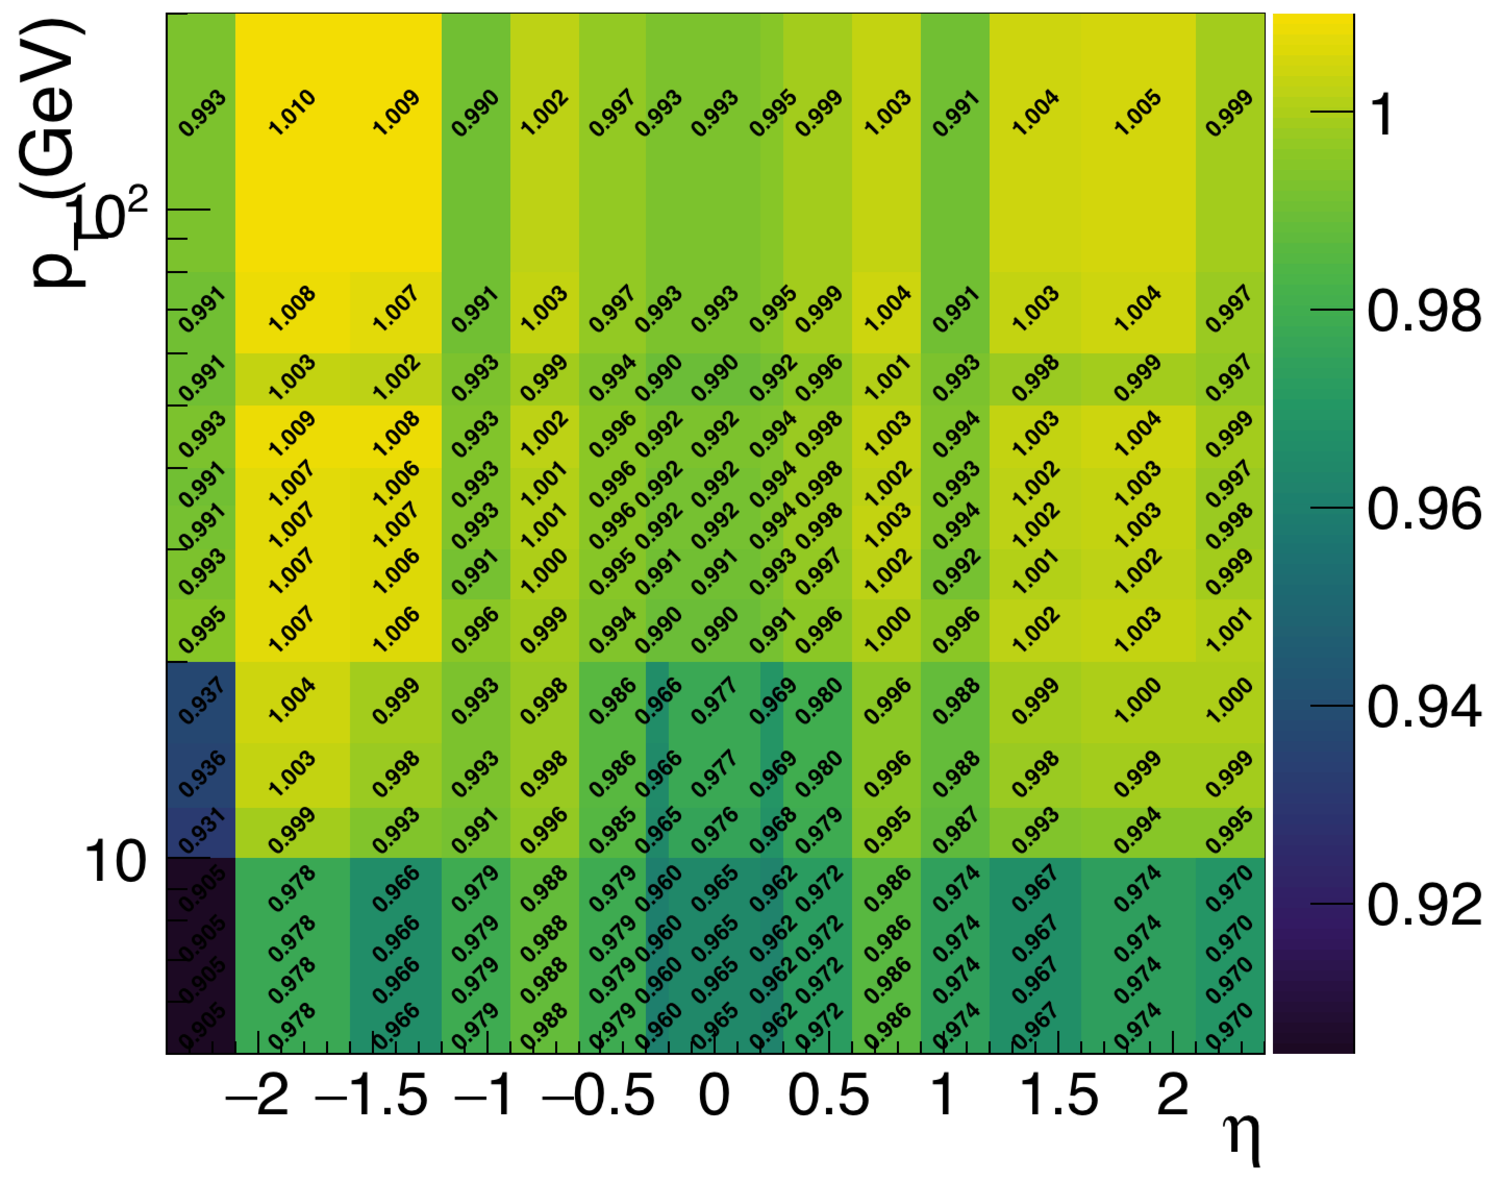
\includegraphics[width=2.5in]{Figures/Muons/mu_sf.pdf}
\caption{}
\end{subfigure}
\begin{subfigure}{0.45\textwidth}
\centering
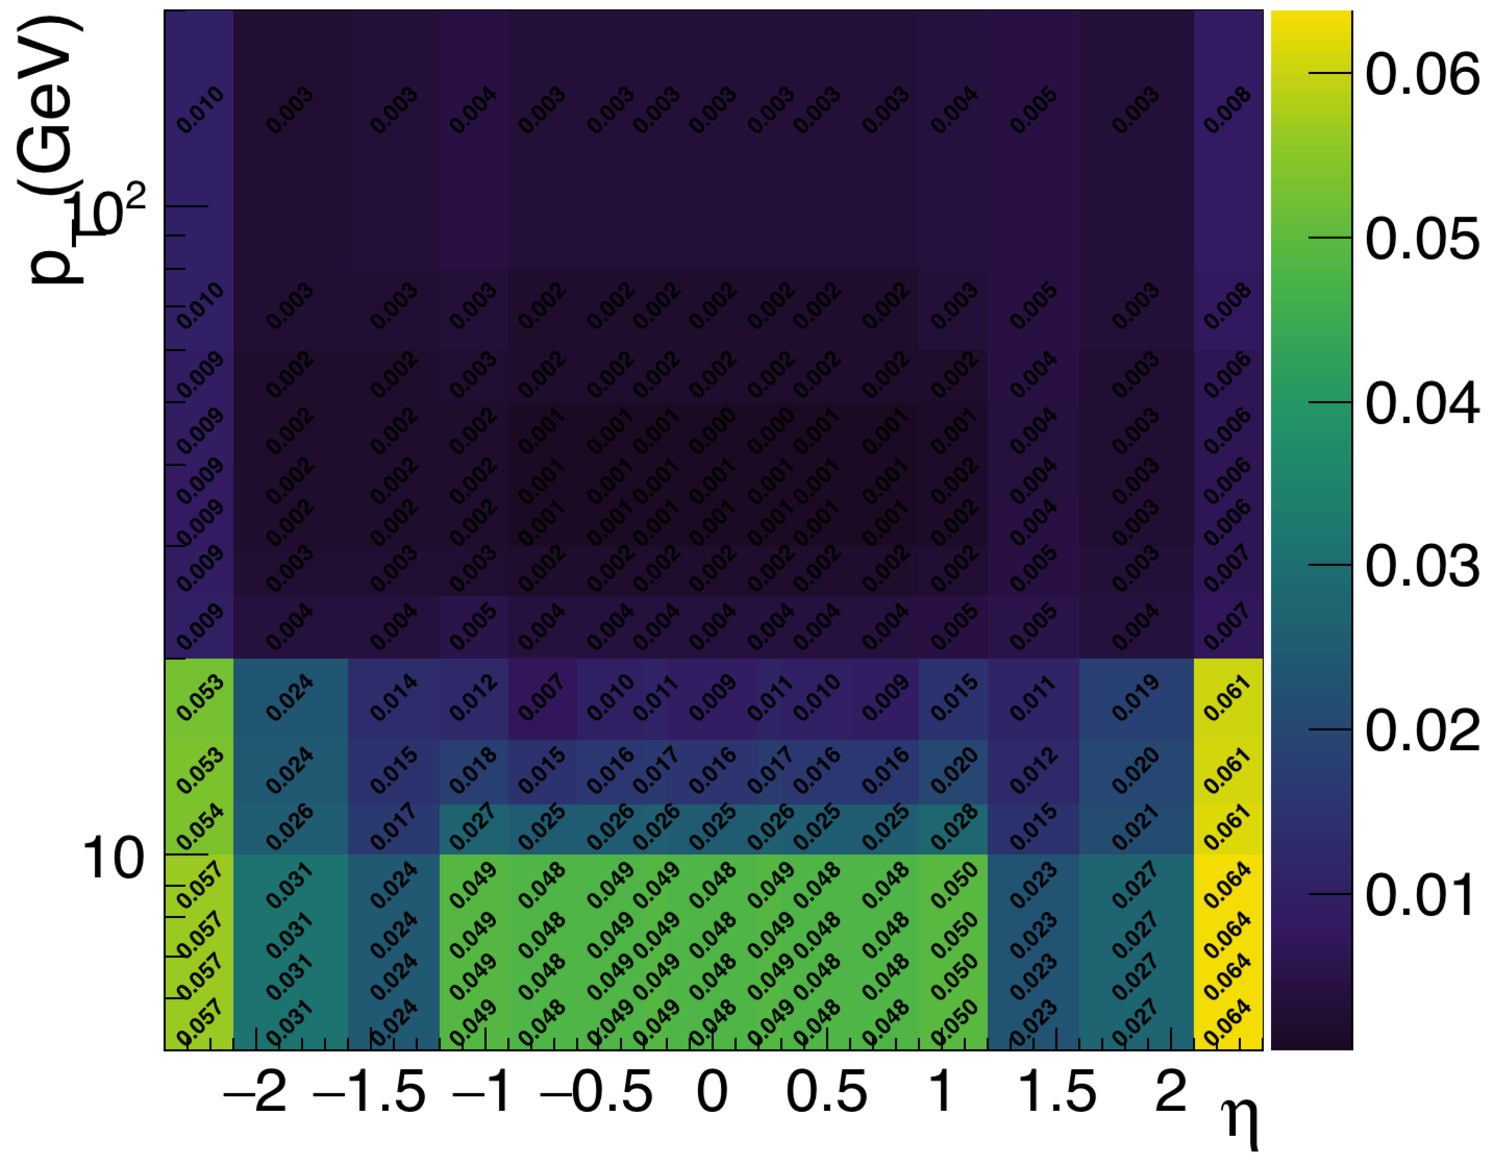
\includegraphics[width=2.5in]{Figures/Muons/mu_sf_unc.pdf}
\caption{}
\end{subfigure}
    \caption{Left: Overall data to simulation scale factors for muons, as function of \pt and $\eta$. Right: Uncertainties on  data to simulation scale factors for muons, as function of \pt and $\eta$.}
    \label{fig:MuonIDEff_5}
\end{figure}

%\begin{figure}[htbp]
%  \begin{center}
%    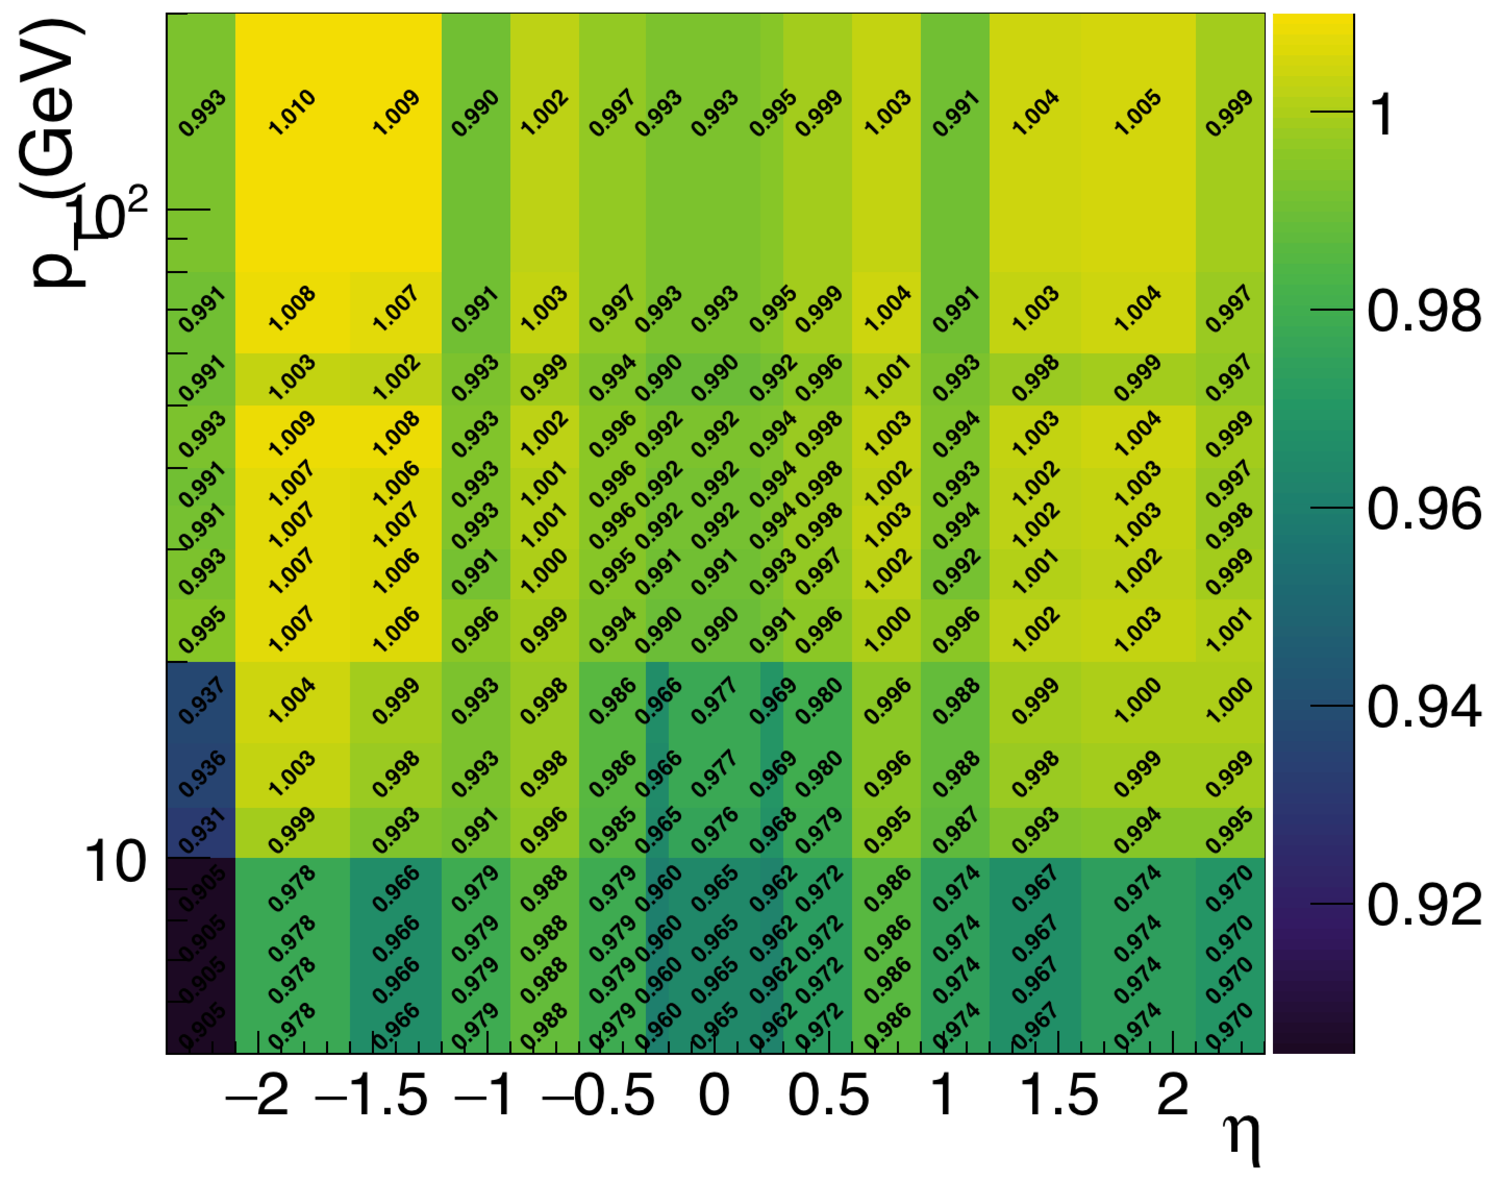
\includegraphics[width=0.45\textwidth]{Figures/Muons/mu_sf.pdf}
%    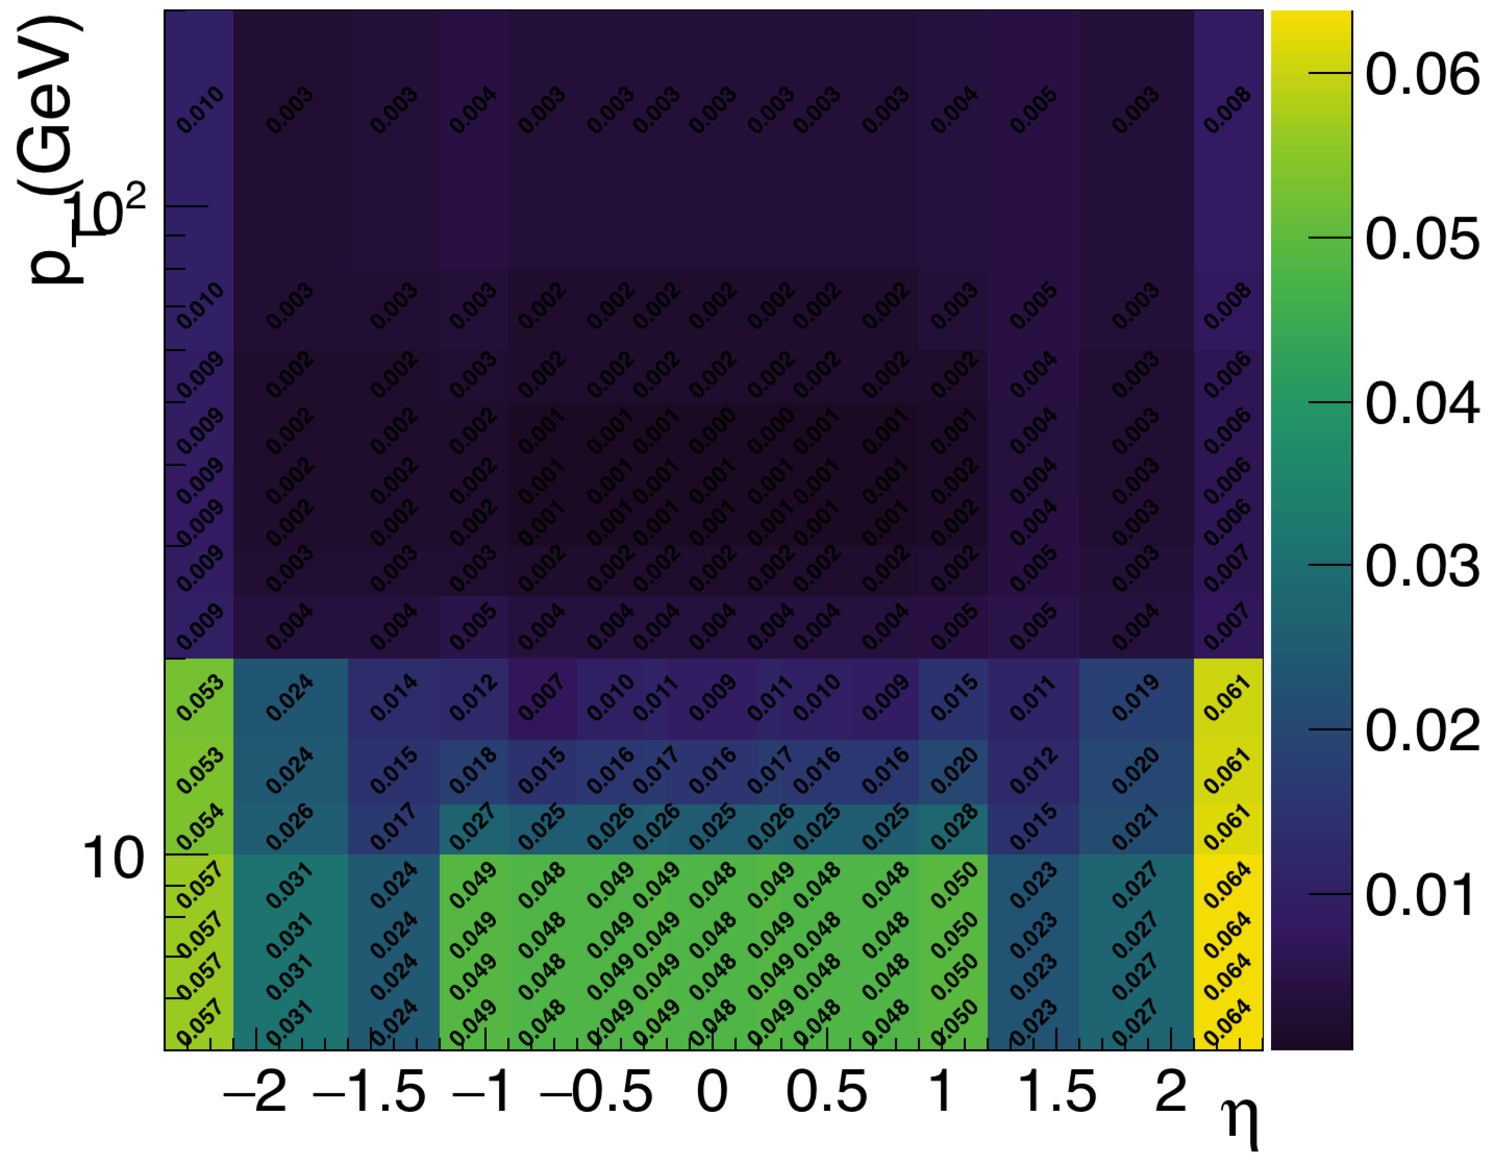
\includegraphics[width=0.45\textwidth]{Figures/Muons/mu_sf_unc.pdf}
%    \caption{Left: Overall data to simulation scale factors for muons, as function of \pt and $\eta$. Right: Uncertainties on  data to simulation scale factors for muons, as function of \pt and $\eta$.}
%    \label{fig:MuonIDEff_5}
%\end{center}
%\end{figure}


\section{Photons for FSR recovery}
\label{sec:FSRphotons}

The FSR recovery algorithm was considerably simplified with respect to what was done in Run I, while maintaining similar performance. 
The selection of FSR photons is now only done per-lepton and no longer depends on any Z mass criterion, thus much simplifying the subsequent ZZ candidate building and selection. As regards the association of photons with leptons, the rectangular cuts on $\Delta R(\gamma,l)$ and $E_{T,\gamma}$  have been replaced by a cut on $\Delta R(\gamma,l)/E_{T,\gamma}^{2}$.

Starting from the collection of 'PF photons' provided by the particle-flow algorithm, the selection of photons and their association to a lepton proceeds as follows:
\begin{enumerate}
\item The preselection of PF photons is done by requiring $p_{T,\gamma} > 2~\GeV$, $|\eta^{\gamma}| < 2.4$, and a relative Particle-flow isolation smaller than $1.8$. The latter variable is computed using a cone of radius $R=0.3$, a threshold of $0.2~\GeV$ on charged hadrons with a veto cone of $0.0001$, and $0.5~\GeV$ on neutral hadrons and photons with a veto cone of $0.01$, also including the contribution from pileup vertices (with the same radius and threshold as per charged isolation) .
\item Supercluster veto: we remove all PF photons that match with any electron passing both the loose ID and SIP cuts. The matching is peformed by directly associating the two PF candidates.
\item Photons are associated to the closest lepton in the event among all those pass both the loose ID and SIP cuts.
\item We discard photons that fail the cuts $\Delta R(\gamma,l)/E_{T,\gamma}^2 < 0.012$, and $\Delta R(\gamma,l)<0.5$.
\item If more than one photon is associated to the same lepton, the lowest-$\Delta R(\gamma,l)/E_{T,\gamma}^2$ is selected.
\item For each FSR photon that was selected, we exclude that photon from the isolation sum of all the leptons in the event that pass both the loose ID and SIP cuts. This concerns the photons that are in the isolation cone and outside the isolation veto of said leptons ($\Delta R < 0.4$ AND $\Delta R > 0.01$ for muons and $\Delta R < 0.4$ AND ($\eta^{\text{SC}} < 1.479$ OR $\Delta R > 0.08$) for electrons).
\end{enumerate}

More details on the optimization of the FSR photon selection can be found in Ref.~\cite{AN-15-277, AN-16-217}.

\section{Jets}
\label{sec:jets}

Vector Boson Fusion (VBF) and other production mechanisms of Higgs Boson normally differ as regards the jet kinematics. 
In this analysis, jets are thus used for the event categorization, which will be introduced in Section~\ref{sec:categorization}.

\subsubsection{Jet Identification}

Jets are reconstructed by using the anti-$k_T$ clustering algorithm out of particle flow candidates, with a distance parameter $R = 0.4$, 
after rejecting the charged hadrons that are associated to a pileup primary  vertex.

To reduce instrumental background, the loose working point jet ID suggested by the JetMET Physics Object Group is applied. 
In this analysis, the jets are required to be within $|\eta| < 4.7$ area and have a transverse momentum above 30 GeV. 
In addition, the jets are cleaned from any of the tight leptons (passing the SIP and isolation cut computed after FSR correction) 
and FSR photons by a separation criterion: $\Delta R(\text{jet,lepton/photon}) > 0.4$.


\subsubsection{Jet Energy Corrections}

The calorimeter response to particles is not linear
and it is not straightforward to translate the measured jet energy
to the true particle or parton energy, therefore we need Jet Energy Corrections.
In this analysis, standard jet energy corrections are applied to the reconstructed jets,
which consist of L1 Pileup, L2 Relative Jet Correction,
L3 Absolute Jet Correction for both Monte Carlo samples and data,
and also residual calibration for data.

% Figure~\ref{fig:jets} shows the comparisoin between data and MC for the leading jet in Z events with exactly one jet,
% where a selection $\Delta\phi(Z,{\rm jet})>2.5$ has been applied.

% \begin{figure}[!h]
% \centering
% \includegraphics[width=0.49\linewidth]{Figures/Jets/Histo_etaj1_2e_dataeff.pdf}
% \includegraphics[width=0.49\linewidth]{Figures/Jets/Histo_etaj1_2mu_dataeff.pdf}
% \caption{Comparison between data and MC for jet $\eta$ in Z + 1 jet events. \label{fig:jets}}
% \end{figure}


\subsubsection{B-tagging}

For categorization purpose, we need to distinguish whether a jet is b-jet or not.
The \emph{Combined Secondary Vertex} algorithm is used as our b-tagging algorithm.
It combines information about impact parameter significance,
the secondary vertex and jet kinematics.
The variables are combined using a likelihood ratio technique to compute the b-tag discriminator.
In this analysis, a jet is considered to be b-tagged if it passes the \emph{CSVv2M} working point,
i.e. if its \verb|pfCombinedInclusiveSecondaryVertexV2BJetTags| discriminator is greater than 0.8484~\cite{btagReferenceEffsRun2}.

Data to simulation scale factors for b-tagging efficiency are provided for this working point for the full dataset as a function of jet $\pt$, $\eta$ and flavour.
They are applied to simulated jets by downgrading (upgrading) the b-tagging status of a fraction of the b-tagged (untagged) jets that have a scale factor smaller (larger) than one.

\section{MET}

The missing transverse energy, $E_{\rm{T}}^{\rm{MISS}}$ or MET, of an event is defined as the magnitude of the imbalance of momentum in the plane transverse to the beam line. Since momentum is conserved in this plane, any imbalance in momentum is attributed to particles escaping the detector without interacting with the detector material, such as neutrinos or hypothetical dark matter candidates. Raw MET or particle flow MET (PFMET) is defined as the magnitude of the negative vectorial sum of the transverse momentum of all reconstructed particle flow candidates, or

\begin{equation}
\overrightarrow{E}_{\rm{T}}^{\rm{MISS}} = - \sum_{i \in \rm{all}} \overrightarrow{p}_{\rm{T},\ i}
\end{equation}

The vector quantity that is the negative sum of reconstructed particle momenta is sometimes called the missing transverse momentum, although this term is used interchangably with its magnitude, the MET. 

An alternative definition of the MET, called the type-I corrected MET, takes into account the jet energy corrections (JEC), correcting for mismeasurment of MET due to detector inefficiencies and non linear responses in the calorimeters. The type-I corrected MET definition is given in Equation~\ref{eq:t1met}. Systematic uncertainties related to modelling real MET are obtained by varying the JEC and jet energy resolution (JER) and measuring the propogation of these variations to the MET uncertainty. These measurements are described in greater detail in the next section.

\begin{equation}
\label{eq:t1met}
\overrightarrow{E}_{\rm{T\ Type-I}}^{\rm{MISS}} = - \sum_{jet} \overrightarrow{p}_{\rm{T},\ jet}^{\rm{JEC}} - \sum_{i \in \rm{uncl.}} \overrightarrow{p}_{\rm{T},\ i}
\end{equation}

where the total contribution has been split into contributions from jets (first term) and contributions from unclustered objects (second term). The transverse momenta of jets in the first term is then replaced with the JEC transverse momenta.

\subsubsection{MET filters}

Due to detector and instrumental noise, several filters are applied to veto noisy events \cite{mettwiki}:

\begin{itemize}
\item HBHENoiseFilter
\item HBHENoiseIsoFilter 
\item EcalDeadCellTriggerPrimitiveFilter 
\item goodVertices 
\item eeBadScFilter 
\item globalTightHalo2016Filter 
\item BadPFMuonFilter 
\item BadChargedCandidateFilter
\end{itemize}

The first two filters remove noisy events from the HCAL, where the HBHE scintillator produce anamolous signals with pulse shapes and pixel multiplicities discrepant from those from a clean signal. The EcalDeadCellTriggerPrimitiveFilter removes events with down ECAL data links, comparing the sum of energy deposited in each cell of a supercluster to the trigger primitive saturation energy. goodVertices removes events with noisy vertex reconstruction from pileup effects. The eeBadScFilter removes events with noisy ECAL end cap super clusters. globalTightHalo2016Filter removes events with enhanced MET from beam-halo particles which are in time with the beam. The last two filters remove events with mis-reconstructed muon and charged hadron particle flow candidates.

\subsubsection{Fake MET modeling}\label{sec:fakemet}

Figure~\ref{fig:pfmet_m4lblinded} shows a discrepancy between data and MC in the high-$E_{\rm{T}}^{\rm{MISS}}$ tail. These events typically contain a high $p_T$ object either back-to-back or collinear with the $E_{\rm{T}}^{\rm{MISS}}$, pointing to artificially high $E_{\rm{T}}^{\rm{MISS}}$ from mismeasurement of the object. These fake events are identified and removed by studying distributions of the transverse angular difference between the MET and various objects in the event \cite{CMS-AN-15-203}.

\begin{figure}[tbh]
\centering
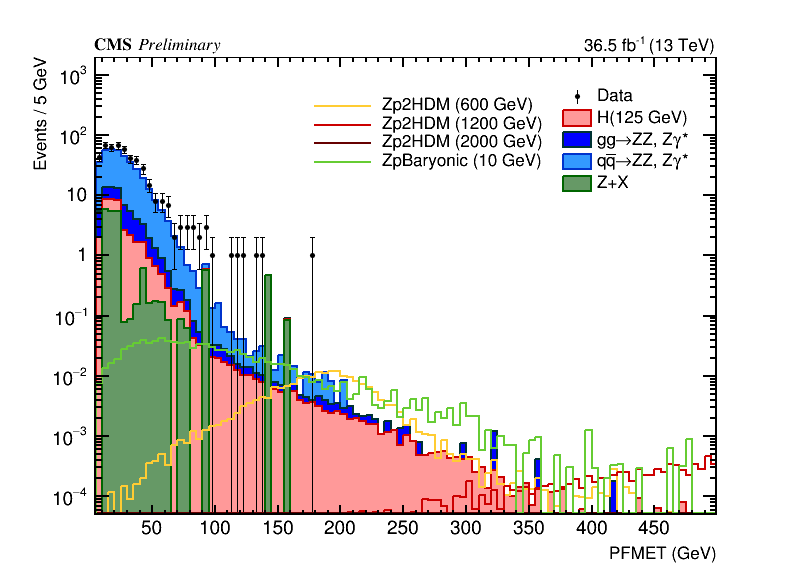
\includegraphics[width=5in]{figures/hist_hPFMET_8.png}
\caption{Missing transverse energy after SM selection before removal of fake MET.}
\label{fig:pfmet_m4lblinded}
\end{figure}

Several variables are studied in order to understand how to remove these fake events from data:

\begin{itemize}
  \item $max|\Delta\phi(jet, E_{\rm{T}}^{\rm{MISS}})|$ with the maximum taken over selected jets, Figure~\ref{fig:maxdeltaphijmet}
  \item $min|\Delta\phi(jet, E_{\rm{T}}^{\rm{MISS}})|$ with the minimum taken over selected jets, Figure~\ref{fig:mindeltaphijmet}
\end{itemize}

The max variables are to check for the occurance of objects with mismeasured energy back-to-back with the MET, the min variable is to check for jets with mismeasured energy collinear with the MET.

\begin{figure}[tbh]
\centering
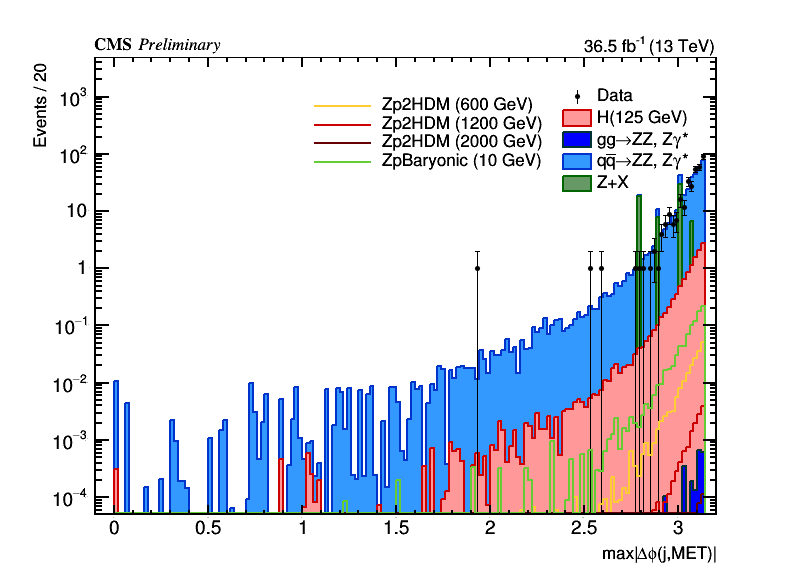
\includegraphics[width=5in]{figures/hist_hDPHI_MAX_JET_MET_8.png}
\caption{Maximum azimuthal angle difference between MET and jets.}
\label{fig:maxdeltaphijmet}
\end{figure}

\begin{figure}[tbh]
\centering
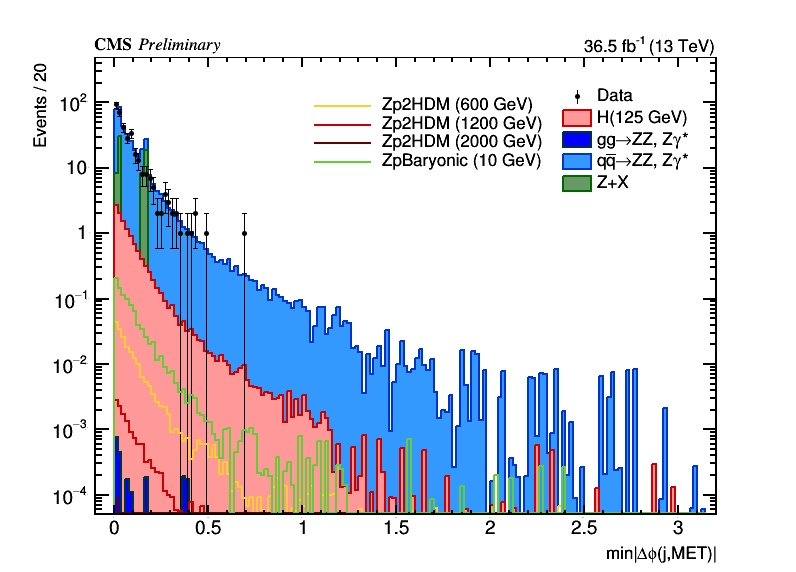
\includegraphics[width=5in]{figures/hist_hDPHI_MIN_JET_MET_8.png}
\caption{Minimum azimuthal angle difference between MET and jets.}
\label{fig:mindeltaphijmet}
\end{figure}

For jets with a high transverse momentum, greater than 50 GeV, it is required that $max|\Delta\phi(jet, E_{\rm{T}}^{\rm{MISS}})|<2.7$ and $min|\Delta\phi(jet, E_{\rm{T}}^{\rm{MISS}})|>0.5$ to exclude events with large MET from mismeasurment of jet energies. These cuts are based on the Run 1 SM analysis selection, chosen to balance the small loss in signal efficiency with the increased systematic uncertainty from mismodelling of the MET in background MC simulations (described in Section~\ref{sec:metsyst}).

